 \documentclass [12pt,letterpaper]{report}
% Add twoside for two-sided printing

% Standard packages
\usepackage{amsmath,amsfonts,amssymb,bm}         % Extra math definitions
\usepackage{graphics}        % PostScript figures
\usepackage{graphicx}        % jpg & png figures
\usepackage{rotating}
\usepackage{setspace}        % double spacing
\usepackage{longtable}       % Tables spanning pages
\usepackage{epigraph}        % Epigraphs
%\usepackage{cite}
\usepackage{here}            % Figure and table placement
%\usepackage[final]{graphicx}
%\usepackage{epsfig}
\usepackage{threeparttable} % Three part tables - allows footnotes for tables
\usepackage{epsf}
%\usepackage[T1]{fontenc}
%\usepackage{times}
\usepackage{psfrag}
\usepackage{rotating}
\usepackage{amsfonts}
\usepackage{float}
\usepackage{enumerate}
%\usepackage{stfloats}
%\usepackage{amssymb}
%\usepackage{amsxtra}
%\usepackage{epic}
%\usepackage{theorem}
%\usepackage{exscale}

% Custom packages
%-----------------------
%\usepackage{authblk}
\usepackage{hyperref}
\hypersetup{
    colorlinks=true,
    linkcolor=blue,
    filecolor=blue,      
    urlcolor=blue,
    citecolor=blue,
}
\usepackage{natbib}  			% Citation
%\usepackage{url}
\usepackage{multirow}
\usepackage{empheq}

\usepackage{slashbox}

\def\acknowledgments{\paragraph*{Acknowledgments.}}

%% tables, to make correct space around the horizontal lines at the
%% top, underneath the column headers, and at the bottom of the table.
\def\topline{\hline\hline\vrule height 10pt depth4pt width0pt\relax}
\def\midline{\hline\vrule height 10pt width0pt\relax}
\def\botline{\hline}
%-----------------------
\usepackage[first]{datestamp}   % Datestamp on first page of each chapter
\usepackage[fancyhdr]{McECEThesis}  % Thesis style
\usepackage{McGillLogo}     % McGill University crest
% $Id: ThesisEx.tex,v 1.1 2005/06/09 12:48:46 kabal Exp $

\usepackage{color}
\def\headrulehook{\color{red}}      % Color the header rule

%===== page layout
% Define the side margins for a right-side page
\insidemargin = 1.0in
\outsidemargin = 1.0in

% Above margin is space above the header
% Below margin is space below footer
\abovemargin = 0.8in
\belowmargin = 0.7in

%========= Document start

\begin {document}

%===== Title page

\title{Impacts of Turbulence on Cloud Microphysics and Warm-Rain Initiation}
\author{Sisi Chen (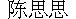
\includegraphics[width=0.15\textwidth]{Chinese_name.pdf})}
\date{\Month\ \number\year}
\organization{%
  \\[0.2in]
  \McGillCrest {!}{1in}\\   % McGill University crest
  \\[0.1in]
  Department of Atmospheric \& Oceanic Sciences\\
  McGill University\\
  Montreal, Canada}
\note{%
  {\color{red} \hrule height 0.4ex}
  \vskip 3ex
  A thesis submitted to McGill University in partial fulfillment of the
  requirements for the degree of Doctorate of Philosophy in Atmospheric Sciences.
  \vskip 3ex
  \copyright\ \the\year\ Sisi Chen

}

\maketitle

%===== insert blank page
\thispagestyle{empty}
\mbox{}
\newpage

%===== Justification, spacing for the main text
\raggedbottom
\onehalfspacing
\pagenumbering{roman}


%===== Abstract, Sommaire & Acknowledgments

\doublespacing
\section*{\centering EPIGRAPH}

\begin{center}
\large \emph{Its five-year mission: to explore strange new worlds, to seek out new life and new civilizations. to boldly go where no man has gone before.} 
\end{center}

\rightline{\textit{--- Captain Kirk   }}
\newpage
\section*{\centering ACKNOWLEDGEMENTS}

Your acknowledgement here.


\newpage
\section*{\centering CONTRIBUTION OF AUTHORS}

The thesis that follows consists of five chapters: an introduction, three original articles, and a conclusion. The three articles have been published in the Journal of the Atmospheric Sciences and Atmospheric Chemistry and Physics. I conducted the research and wrote the manuscripts of all three papers, as part of my Ph.D. studies. The work described in Chapter \ref{sec:ch2} was performed in collaboration with Dr. P.A. Vaillancourt at Environment and Climate Change Canada (ECCC) and the work described in Chapter \ref{sec:ch4} was performed in collaboration with Dr. Lulin Xue at the National Center for Atmospheric Research (NCAR). The articles I included in this thesis reflect suggestions, comments and editorial help from all co-authors.


\newpage
\section*{\centering STATEMENT OF ORIGINALITY}

The following elements of the thesis show original scholarship and represent distinct contributions to knowledge:

\begin{itemize}
\item The work described in Chapter \ref{sec:ch2} on the direct numerical simulation (DNS) studies covers a wide range of turbulence intensities and computational domain sizes. The study is the first to show that the Reynolds number, $R_\lambda$, in DNS experiments is only computational and should not be included in the parameterization of the turbulent collision kernel. An improved parameterization independent of the computational Reynolds number was formulated.

\item The article in Chapter \ref{sec:ch3} offers one of the first comprehensive and quantitative DNS studies of turbulent collision efficiency for droplets prior to their effective gravitational-collisional growth stage ($r<30 \mu m$). In addition, realistic liquid water contents (LWCs) and droplet number concentrations comparable to that of cumulus clouds were used. Finally, the article presents the first attempt to simulate directly droplet growth by collision-coalesence using DNS to allow a quantitative evaluation of the broadening of the entire droplet size distribution (DSD) in various turbulent environments.

\item The study in Chapter \ref{sec:ch4} provides the first complete DNS study of continuous droplet growth by condensation and collision-coalescence under various turbulent conditions. The tools developed in this study provides a direct and accurate approach to attack the challenging problem of the condensation-collision size gap. 

\end{itemize}

\newpage
\section*{\centering ABSTRACT}
In shallow cloud systems, such as cumulus or stratocumulus clouds, broad droplet size spectra and fast rain formation times are frequently observed using radar and in-situ measurements. However, these observations cannot be represented by classical condensational growth theory. Turbulence has been hypothesized to accelerate the formation of raindrops by enhancing the cloud droplet collision-coalescence process. In this thesis, the direct numerical simulation (DNS) approach is used to investigate the role of turbulence in cloud microphysics processes during warm-rain initiation and to quantify the effect of turbulence on the collision rate between droplets. We developed an accurate and sophisticated modeling framework that couples dynamics and thermodynamics, thus allowing the incorporation of droplet growth by simultaneous condensational and collisional processes under various turbulent conditions. 

Throughout the thesis, three sets of numerical experiments are conducted to study the turbulence impact on various droplet growth processes: 1) the droplet geometric collision, i.e., collisions without considering the disturbance flow induced by the presence of droplets, 2) the droplet hydrodynamic collisions, by including the disturbance flow, and 3) the interactions between condensational growth and collisional growth by further including the thermodynamic fields. 

The results of the first two sets of experiments demonstrate that for droplet pairs with different sizes ($r_1/r_2<0.8$), turbulence plays a dominant role in modifying the droplet hydrodynamic response to the local disturbance flow, weakly increasing the droplet relative velocity and creating clustering of droplets in space. Consequentially, a significant enhancement of the collision efficiency and a mild enhancement of geometric collision kernel resulted. On the other hand, for droplet pairs with similar sizes ($r_1/r_2>0.8$), the turbulence enhancement in geometric collision and droplet hydrodynamic interactions is strong. Since droplet condensational growth produces a narrow droplet size distribution (DSD), we hypothesize that turbulence effectively widens the narrow spectrum by boosting similar-sized collisions. This hypothesis is further verified by conducting simulations of DSD evolution through collision-coalescence at various flow conditions. It is found that turbulence significantly broadens the DSD, and similar-sized collisions contribute to  21-24\% of the total collisions compared to only 9\% in the still-air experiments. Finally we study the interaction of thermodynamics and dynamics and its impact on droplet growth by allowing droplets to simultaneously grow by condensation and collision in turbulent and non-turbulent environments. The results show that the condensational process promotes collisions in a turbulent environment while it reduces the collisions when in still air, indicating a positive impact of dynamics (turbulence) on the interaction of condensation and collision.

In addition, we investigate the relative importance of different scales of turbulent flow on the collision statistics by varying the computational domain size. It is found that for small droplets ($r < 25 \mu m$), their motions and collisions are mainly affected by the smallest scales of turbulence (i.e. the Kolmogorov length scale) and the large-scale motion has negligible influence on modifying the collision rate. This suggests that on the one hand, turbulent collision statistics can be obtained by using relatively small computational resources, and on the other hand, the computational Reynolds number, $R_\lambda$, should be removed from the parameterization of the turbulent collision kernel. As a consequence, an improved parameterization of droplet turbulent collision kernel is proposed that is highly consistent with the DNS results. 

\newpage

\section*{\centering R\'ESUM\'E}
Dans les syst\`emes de nuages bas, tels que les cumulus ou stratocumulus, des larges distributions de taille de gouttelettes et des temps de formation de pluie rapides sont fr\'equemment observ\'es en utilisant des radars et des mesures in-situ. Cependant, ces observations ne peuvent pas \^etre repr\'esent\'ees par la th\'eorie classique de la croissance par condensation. Une hypoth\`ese sugg\`ere que la turbulence acc\'el\`ere la formation de gouttes de pluie en am\'eliorant le processus de collision-coalescence des gouttelettes de nuage. Dans cette th\`ese, l'approche de simulation num\'erique directe (DNS) est utilis\'ee pour \'etudier le r\^ole de la turbulence dans les processus de microphysique des nuages durant l'initiation de la pluie chaude et quantifier l'effet de la turbulence sur le taux de collision entre gouttelettes. Nous avons d\'evelopp\'e un cadre de mod\'elisation pr\'ecis et sophistiqu\'e qui couple les processus dynamiques et thermodynamiques, permettant ainsi de combiner la croissance des gouttelettes par des processus simultan\'es de condensation et de collision dans diverses conditions turbulentes.

Tout au long de la th\`ese, trois s\'eries d'exp\'eriences num\'eriques sont men\'ees pour \'etudier l'impact de la turbulence sur: 1) le taux de collision g\'eom\'etrique des gouttelettes, 2) le taux de collision hydrodynamique des gouttelettes, notamment l'efficacit\'e des collisions et 3) les interactions entre la croissance de condensation et la croissance collisionnelle (en incluant en plus les champs thermodynamiques).

Les r\'esultats des deux premi\`eres s\'eries d'exp\'eriences montrent que pour les paires de gouttelettes de tailles diff\'erentes ($ r_1/r_2<0.8$), la turbulence joue un r\^ole dominant dans la modification de la r\'eponse hydrodynamique des gouttelettes au flux de perturbation locale et dans la cr\'eation de regroupements de gouttelettes dans l'espace. Cons\'equemment, une am\'elioration significative de l'efficacit\'e de la collision et une l\'eg\`ere am\'elioration du noyau de collision g\'eom\'etrique en r\'esultent. D'autre part, pour les paires de gouttelettes de taille similaire ($r_1/r_2>0.8 $), l'am\'elioration de la turbulence dans les interactions g\'eom\'etriques de collision et dans les interactions de l'hydrodynamiques des gouttelettes est forte. Puisque la croissance par condensation des gouttelettes produit une distribution de la taille des gouttelettes (DSD) qui est \'etroite, nous \'emettons l'hypoth\`ese que la turbulence \'elargit effectivement le spectre \'etroit en augmentant les collisions de taille similaire. Cette hypoth\`ese est en outre v\'erifi\'ee en effectuant une simulation de l'\'evolution DSD par collision-coalescence pour diverses conditions d'\'ecoulement. On constate que la turbulence \'elargit significativement le DSD et que les collisions de taille similaire contribuent \`a 21-24\% des collisions totales contre seulement 9\% dans les exp\'eriences en l'absence de vent. Finalement, nous \'etudions l'interaction de la thermodynamique et de la dynamique et son impact sur la croissance des gouttelettes en permettant aux gouttelettes de croître simultan\'ement par condensation et collision dans des environnements turbulents et non-turbulents. Les r\'esultats montrent que le processus de condensation favorise les collisions dans un environnement turbulent tout en r\'eduisant les collisions en l’absence de vent, indiquant un impact positif de la dynamique (turbulence) sur l'interaction de la condensation et de la collision.

En outre, nous \'etudions l'importance relative des diff\'erentes \'echelles d'\'ecoulement turbulent sur les statistiques de collision en faisant varier la taille du domaine de calcul. On constate que pour les petites gouttelettes ($r<25\mu m$), leurs mouvements et collisions sont principalement affect\'es par les plus petites \'echelles de turbulence (\'echelle de Kolmogorov) et le mouvement \`a grande \'echelle a une influence n\'egligeable sur la modification du taux de collision. Ceci sugg\`ere que d'une part, les statistiques de collision turbulente peuvent \^etre obtenues en utilisant des ressources computationnelles relativement petites, et d'autre part, le nombre de Reynolds de calcul, $R_\lambda $, devrait \^etre retir\'e de la param\'etrisation du noyau de collision turbulent. En cons\'equence, une param\'etrisation am\'elior\'ee du noyau de collision turbulent de gouttelettes est propos\'ee, ce qui est hautement coh\'erent avec les r\'esultats du DNS.




%========== Tables of contents, figures, tables
\tableofcontents
\listoffigures
\listoftables

\newpage

\chapter*{List of Acronyms}\markright{List of Acronyms}
\begin{flushleft}
\begin{longtable}{p{6cm}p{13cm}}
  CCN          &  Cloud Condensation Nuclei\\
  CRM          &  Cloud-System Resolving Model\\
  DF           &  Disturbance Flow\\
  DNS            &  Direct Numerical Simulation\\
  DSD          &  Droplet Size Distribution\\
  EDR          &  Eddy Dissipation Rate\\
  GCM          &  General Circulation Model\\
  LES           &  Large-Eddy Simulation\\
  LWC          &  Liquid Water Content\\
  MPI          &  Message Passing Interface\\
  RDF          &  Radial Distribution Function\\
  RRV          &  Radial Relative Velocity\\
  SCE          &  Stochastic Collision Equation\\
  \emph{pdf}    &  Probability Density Function\\
  \emph{rms}    &  Root-Mean-Square\\
\end{longtable}
\end{flushleft}

\newpage
\chapter*{List of Constants and Symbols}\markboth{List of Constants and Symbols}{List of Constants and Symbols}

The following list the most important symbols used in the thesis. Where relevant, boldface is used to denote vectors or matrices.

~\\\noindent \Large Constants \normalsize
\begin{flushleft}
\begin{longtable}{p{6cm}p{13cm}}
 $C_p=1005 J kg^{-1} K^{-1}$ & Specific heat for air \\
 $D_v=2.55 \times 10^{-5} m^2 s^{-1}$ & Water vapor diffusivity\\
 $D_t=2.22 \times 10^{-5} m^2 s^{-1}$ & Thermal diffusivity\\
 $g=9.8 m/s^2$ & Gravitational constant\\
 $\Gamma_d=-g/C_p$ & Dry adiabatic lapse rate\\
 $K_a=2.48 \times 10^{-2} J m^{-1} s{-1} K^{-1}$ & Thermal conductivity of air \\
 $L=2.477 \times 10^6 J kg^{-1} K^{-1}$ & Specific latent heat for water\\
 $N_{Sc} = \nu / D_v$   & Schmidt number \\
 $\nu = 1.6 \times 10^{-5} m^2 s^{-1}$ & Air kinematic viscosity \\
 $R_v=461.5 J kg^{-1} K^{-1}$ & Individual gas constant for water vapour\\
 $R_a=287 J kg^{-1} K^{-1}$ & Individual gas constant for dry air \\
 $\rho_w = 1000.0 kg m^{-3}$   & Density of water \\

 

\end{longtable}
\end{flushleft}

\noindent \Large Symbols \normalsize
\begin{flushleft}
\begin{longtable}{p{4cm}p{13cm}}
    $C_d$, $C_{dM}$, $C\prime_d$ & Local condensation rate, parcel condensation rate, and condensation rate fluctuation $[kgs^{-1}kg^{-1}]$\\
    $E(r_1,r_2)$ 	& Collision efficiency between droplets $r_1$ and $r_2$\\
    $e_{sat}$            & Saturated water vapor pressure [$Pa$]\\
    $\epsilon$ 		& Eddy dissipation rate [$cm^2 s^{-3}$]\\
    $\eta$ 		& Kolmogorov length scale [m]\\
    $\mathbf{F}$ 	& External forcing maintaining turbulence [$m s^{-2}$]\\
    $f_D$               & Longitudinal correlation function of the velocity derivative\\
    $f_v$               & Droplet ventilation coefficient\\
    $g(R)$ 		& Radial distribution function\\
    $\Gamma$ 		& Collision kernel [$m^3s^{-1}$]\\
    $\mathbf{k}$ 	& Wave vector \\
    $KE$, $KE_{in}$      & Total kinetic energy and amount of kinetic energy injection  [$m^2s^{-2}$]\\
    $L$ 		& Computational domain size in one direction [m]\\
    $\lambda$           & Taylor microscale [$m$]\\
    $\lambda_D$         & Longitude Taylor microscale\\
    $\mu$               & Turbulence intermittent exponent\\
    $N$                 & Number of grid points\\
    $\Omega$ 		& Computational domain size [$m^3$]\\
    $P$ 		& Pressure [Pa]\\
    $q_v$, $q_v\prime$, $q_{vs}$      & Water vapor mixing ratio, water vapor mixing ratio flucutaion, and saturated water vapor mixing ratio [$kgkg^{-1}$] \\
    $\rho_a$		& Air density [$kgm^{-3}$]\\
    $R_\lambda$   	& Taylor microscale Reynolds number\\
    $Re_p$ 		& Droplet Reynolds number\\
    $\tau_p$ 		& Particle response time [s]\\
    $\tau_k$ 		& Kolmogorov timescale [s]\\
    $r$, $r_1$, $r_2$   & Radius of droplet [m]\\
    $R$ 		& Sum of radius $r_1$ and $r_2$\\
    $St$ 		& Stokes number\\
    $T, T\prime$        & Temperature and temperature fluctuation [$K$]\\
    $u\prime$           & $rms$ velocity [$ms^{-2}$]\\
    $\mathbf{U}$ 	& Turbulent flow velocity [$m/s$]\\
    $\mathbf{V_t}$ 	& Droplet terminal velocity [$m/s$]\\
    $\mathbf{V}$ 	& Droplet velocity [$m/s$]\\
    $\mathbf{W_r}$ 	& Droplet radial relative velocity [$m/s$]\\
    $\mathbf{W}$ 	& Droplet relative velocity [$m/s$]\\
    $W\prime$           & Vertical perturbation velocity[$ms^{-1}$]\\
    $x_0$               & Critical separation distance in gravitational collision kernel [$m$]\\
    $Z$                 & Total enstrophy [$s^{-2}$]\\
\end{longtable}
\end{flushleft}

%\noindent \Large Sets \normalsize
%\begin{flushleft}
%\begin{longtable}{p{2cm}p{13cm}}
%    $\mathbb{B}$ & Set of binary numbers\\
%    $\mathbb{R}$ & Set of real numbers\\
%    %$\mathbb{Z}$ & Set of real numbers\\
%\end{longtable}
%\end{flushleft}

\cleardoublepage
\pagenumbering{arabic}


%========== Chapters
\typeout{Introduction}
\resetdatestamp

\chapter{Introduction}

%\epigraph{A change in the weather is sufficient to recreate the world and ourselves.}{\emph{Marcel Proust} (1871 -- 1922)}

\section{Background}



\subsection{Clouds, weather, and climate}
	
Shallow convective clouds, such as marine stratocumulus clouds and trade-wind cumuli, represent an important component of the weather and climate systems of the Earth. In the first place, they substantially influence the Earth's radiation budget by reflecting the incoming short-wave radiation. This cooling of the atmosphere affects the large-scale dynamics as a response to the decreased radiative forcing. For example, the albedo of shallow marine clouds in the tropical and subtropical regions is about 0.3-0.8 \citep{ Chen2012, Painemal2012}, more than fivefold larger than the albedo of the ocean surface \citep [$\approx$ 0.06-0.1,] []{Payne1972}. However, by virtue of their shallowness and closeness to the ocean surface, these clouds radiate at nearly the same intensity as the surface and do not contribute to modulating the outgoing longwave radiation \citep{Stevens2009}. Consequently, shallow clouds have a strong net radiative effect, which in turn greatly impacts the intensity and distribution of storm-tracks in the mid-latitudes \citep{Wang2014} and the rain belts in the Inter Tropical Convergence Zone (ITCZ) \citep{Voigt2016}.

Secondly, clouds have a determinant influence on the Earth's hydrological cycle by redistributing the water on the planet through the interaction with atmospheric circulation and the processes of precipitation. Rain produced from warm clouds accounts for 31\% of the total rainfall on the planet and 72\% of the total rain area in tropical regions \citep{Lau2003}. The warm-rain processes can sometimes even result in natural hazards. For instance, the 2013 Great Colorado Flood along the eastern slopes of the Colorado Rocky Mountains was mainly caused by an unusually severe warm-rain process. During the event, a large concentration of small-sized raindrops and a copious amount of precipitable water were observed \citep{Friedrich2016}. 18 counties impacted by the floods were declared by the Federal Emergency Management Agency (FEMA) as federal disaster areas and damages exceeding \$2 billion in U.S. dollars were produced \citep{Gochis2013}. 

\subsection{Warm-rain initiation and condensation-collision size gap}

It is widely accepted that the growth process of a droplet in warm clouds consists of three basic sub-processes \citep[e.g., ][]{Rogers1989} : 1) droplets form from the activation of cloud condensation nuclei (CCN); 2) droplets grow by diffusion of water vapor (condensation); 3) droplets grow by collision-coalescence. For condensation, the approximate growth rate of a droplet in radius is inversely proportional to its size but directly proportional to the supersaturation in its immediate environment when solute and curvature effects are neglected, viz.
\begin{equation}
\frac{dr}{dt}\propto \frac{S}{r},
\end{equation}
where $S$ is the supersaturation and $r$ the droplet radius. The implication is that small droplets grow faster than large droplets. As a consequence, two droplets starting with different sizes would grow to a similar size in the end. It is known that the process of condensational growth dominates until a droplet reaches around 15 $\mu m$ in radius \citep{Pruppacher1997}. For larger droplets, the collision process takes over to form raindrops. In still air collision occurs when heavier droplets capture smaller ones lying in their paths under the influence of gravity. To initiate the collisional process effectively, a broad droplet size distribution (i.e., the co-existence of big drops and small droplets) is required. In general, droplets need to grow to at least 30-40 $\mu m$ for the gravitational collisional process to be effective \citep{Mason1975, Grabowski2013}. The underlying reason is that before this stage, the relative fall speed between droplets is very small and the collision efficiency becomes negligible. Specifically, when a droplet moves relative to the flow, a local flow field around the droplet surface called the disturbance flow is generated. The disturbance flow causes two approaching droplets to have a tendency to move away from each other and avoid collision. In particular, small droplets have weak inertia and tend to follow streamlines and thus have a low probability of collision, or a low collision efficiency. As a consequence, a condensation-collision size gap ($r \approx 15-30 \mu m$) exists where both condensational growth and collisional growth are inefficient.

However, radar observations show that warm rain can form within 15-20 minutes \citep{Szumowski1997, Knight2002, Goke2007}. and heavy precipitation \citep{Stevens2016} and wide droplet size distributions (DSDs) \citep{Warner1969, GRL2017,Siebert2017, Witte2017} have frequently been observed in shallow convective systems. Nevertheless, classical condensational growth theory for an air parcel rising adiabatically from the cloud base fails to reproduce the observed features in a reasonable timescale due to the growth size gap \citep{Jonas1996}.

\subsection{Possible mechanisms to broaden the droplet size spectrum}

The conflicting results between observation and theory pose a challenge for the cloud physics community for decades. In the literature, several mechanisms have been proposed to explain how warm-rain can be initiated efficiently. They include small-scale turbulence, aerosol effects, and cloud-scale mixing. Interested readers may refer to the review articles by \citet{Vaillancourt2000}, \citet{Devenish2012}, and \citet{Grabowski2013} for a comprehensive overview of these mechanisms. Here, a brief summary is given below.

\subsubsection{Small-scale turbulence}

Turbulence, though difficult to define precisely, is characterized by its randomness, intermittency, multi-scale interactions, and features of dissipation, diffusion and mixing \citep{TL1972}. Turbulence is ubiquitous in nature. Cumulus clouds are turbulent. Laboratory experiments \citep[e.g., ][]{Bordas2013} and numerical modeling studies \citep[e.g., ][]{Wang2000, Wang2008} have yielded evidence that turbulence may enhance cloud droplet collision-coalescence growth when the droplets are still small. The large eddy simulation (LES) experiments performed by \citet{Wyszogrodzki2013} show that turbulence can shorten the initiation time of warm rain and increase the amount of rainfall. 

So far, three major effects of turbulence have been found crucial to enhance the probability for collision or the collision kernel \citep{Wang2009}: 
(1) Turbulence redistributes droplets in space and thus creates droplet clustering (i.e., the turbulence clustering effect which affects the radial distribution function); (2) turbulence increases the droplet relative motion and modifies the droplet settling velocity (i.e., the transport effect); (3) turbulence modifies the droplet hydrodynamic response to the local disturbance flow which is induced by the flow passing by the droplet surface. This is so-called the turbulence hydrodynamic effect. The overall enhancement of turbulence through the above three mechanisms depends on the intensity of turbulence and the size of the droplets. 

\subsubsection{Aerosol effects}

Aerosols, including natural -- sulfates, sea salt, organic aerosols, etc. -- and anthropogenic -- soots, cloud seeding materials, etc. -- are the most common cloud condensation nuclei. Arguably, the physical and chemical properties of aerosols not only affect the cloud macroscopic properties such as the optical property \citep{Twomey1959}, cloud lifetime \citep{Albrecht1989, Small2009}, and cloud morphology \citep{Jiang2009}, but also affect the microscopic properties such as the hygroscopicity (solute effect) and particle growth rate. It is often assumed in many cloud models and microphysics schemes \citep[e.g., ][]{Morrison2005, Thompson2014} that the size of the CCN is relatively small. Therefore, the hygroscopic contribution of CCNs is only considered in the droplet activation process but is omitted in subsequent droplet growth in clouds. Studies such as \citet{Jensen2017} and \citet{blyth2003} found that giant CCN, or GCCN (with a dry radius $> 0.5 \mu m$), mostly observed in marine regions where breaking waves generate giant sea-salt particles, may accelerate condensational growth and act as raindrop embryos.

\subsubsection{Cloud-scale mixing}

As the condensational growth rate of a droplet is mainly associated with its local supersaturation, it has been argued that the fluctuating supersaturation resulting from turbulent fluctuations in the vertical wind can have a large effect on the evolution of the DSD. The first theoretical framework describing this effect was developed by \citet{cooper1989}. He proposed that droplets ending up at the same location within a turbulent cloud can encounter different Lagrangian trajectories and thus experience various condensational growth histories to broaden the DSD. The effect was later coined as "eddy hopping" by \citet{Grabowski2013} to describe the process of a droplet hopping from one large eddy to another and thus experiencing variation of supersaturation along the droplet trajectory. \citet{grabowski2017} demonstrated via a turbulent adiabatic parcel model that turbulence can virtually suppress the DSD narrowing effect during condensational growth. 

\subsection{Entrainment and mixing at the cloud edge}
Another mechanism associated with the effect of mixing on droplet condensational growth is the entrainment near the cloud edge. In the entraining cloud region cloudy and unsaturated air meets and droplets exposed to unsaturated air evaporate completely while other droplets remain unaffected. The result is a reduction in droplet number concentration and fewer droplets to compete for the available water vapor with subsequent faster condensational growth. This mixing process is known as inhomogeneous mixing as opposed to homogeneous mixing where all droplets partially evaporate at a similar pace so that the mean-droplet radius is reduced but the droplet number concentration remains constant. In addition, the fresh CCN entrained into the cloud lead to secondary activation and further broadening of the droplet distribution towards smaller sizes. Nevertheless, numerical studies show that the formation of raindrops by condensational growth still requires high liquid water content (LWC) after droplets experience entrainment \citep{Twomey1966}. Moreover, evidence is lacking to demonstrate that large droplets resulting from entrainment can be reintroduced into high LWC regions \citep{cooper2013}.


In passing we emphasize that the candidate mechanisms mentioned above are not well-quantified and are difficult to be implemented in microphysics parameterizations. Consequently, inaccurate microphysics parameterizations contribute to a large extent to the poor simulation of cloud properties in various models (e.g., LES, CRM, NWP and climate models) \citep{Fan2016}. Untangling cloud microphysical processes and their interaction with cloud dynamics would go a long way toward improving cloud microphysics parameterizations, prediction of cloud cover and rainfall intensity, and better understanding of cloud feedback on climate. This dissertation aims to contribute towards these goals by scrutinizing the effect of turbulence on microphysics and raindrop formation in warm clouds. 
%The geometric collision kernel is a measure of the rate of collision between two droplet sizes under no hydrodynamic effect. It is the average volume swept out by a collector droplet (the bigger one in the droplet pair) per unit time. Within that volume, collisions are expected to happen.



\section{Outstanding questions in warm cloud microphysics}


The representation of cloud processes, especially in shallow clouds, remains a dominant source of uncertainty in climate models \citep[chapter 7]{ipcc2014}. Due to the coarse resolution in current weather and climate models, cloud microphysical processes involved in the formation and evolution of cloud droplets and raindrops, such as condensation, evaporation, collision, coalescence, and breakup, have to be parameterized. The parameterizations provide the thermodynamic and dynamic feedbacks through latent heating/cooling and mass loading, determine the type and intensity of precipitation at the surface, affect the optical properties of clouds which are crucial to atmospheric radiation, and interact with the chemical and aerosol processes. In cloud models such as LES and cloud system resolving models (CRMs), the microphysical representation is not accurate due to poor understanding of the underlying physical processes. Consequentially, there is no benchmark to gauge the parameterization, leading to poor simulation of cloud properties and poor forecasts of precipitation \citep{Fan2016}. In addition, there is no convergence of model results using different schemes. For example, \citet{White2017} found that the uncertainty caused by using different double-moment bulk schemes under the same model framework even exceeds the aerosol effects due to a poor representation of cloud processes (e.g., autoconversion, saturation adjustment and partitioning of hydrometers). Even though bin schemes are more accurate than bulk schemes (bin models calculate the microphysical quantities of each particle bin for every hydrometer category instead of only computing the momentum of a presumed particle size distribution in bulk models), different bin microphysics schemes still yield a wide spread of dynamic and thermodynamic structures of a squall line, qualitatively similar to the spread produced by bulk schemes \citep{Xue2017}. For models such as the CRM or LES with resolution between 10m-100km, microphysics are parameterized in resolved clouds. In models with coarser grids (> 100 km) such as general circulation models (GCMs), microphysics is parameterized within the parameterized clouds. As such, the uncertainty of microphysics schemes is magnified. Therefore, improving the understanding of cloud microphysical process and their interactions with the environment is urgently needed to improve cloud microphysics parameterizations, to provide better constraints on weather and climate models, and to eventually reduce model uncertainty in cloud processes. 

Specifically, this dissertation is focused on investigating and quantifying the effect of turbulence on droplet growth inside the adiabatic cloud core, in the hope of seeking a more accurate parameterization for describing the warm-rain initiation process. The adiabatic core is a region of a cloud where no entrainment of dry air is found. It is argued that the first raindrops are formed here owing to its higher LWC and more large droplets than the surrounding diluted cloud body \citep{Vaillancourt2001, Khain2013}.  The research questions to be answered by this study are listed below:


1) What is the role of turbulence in droplet geometric collision (i.e., the collision that does not consider hydrodynamic droplet interactions)?  What is the relative importance of different scales of turbulent motion on droplet collisions? Can we quantify the turbulent effects and find an accurate parameterization of the collision rate?

2) How does turbulence impact the droplet hydrodynamic interaction and thus modify the collision efficiency? 

3) How does the condensational process interact with the collisional process in a turbulent environment? How does turbulence modulate such interactions?

4) Finally, how does the droplet size distribution evolve under different turbulent conditions? And how does turbulence modulate the rain formation time?


\section{Methodology}

\subsection{Direct numerical simulation}

To tackle the research questions raised in the previous section, a direct numerical simulation (DNS) approach is employed to simulate the cloud microphysical processes in the turbulent, adiabatic region inside a cumulus cloud, aka. the adiabatic core. In each chapter, the DNS code is modified in such a way that the specific physical processes are resolved to scrutinize the turbulence effect on those processes. The model consists of two components: dynamics (i.e., turbulent flow) and cloud microphysics (i.e., individual droplet Lagrangian movement, detection of droplet collisions, and/or droplet diffusional growth). 

Overall, the DNS aims to simulate explicitly continuous droplet growth in a turbulent, supersaturated environment inside the cloud. The whole computational domain is regarded as an air parcel ascending from the cloud base. The turbulence is generated by solving the incompressible Navier-Stokes equations. The disturbance flow induced by flow passing over the droplet surface is solved and super-imposed onto the turbulent flow such that all droplet-collision-relevant dynamics are appropriately included. For droplets, they are traced in a Lagrangian framework, and their motion is governed by the drag of the flow and the effect of sedimentation (i.e., gravity). To collect the turbulent collision statistics of designated droplet sizes, droplets are not allowed to merge by collision-coalescence (Chapter \ref{sec:ch2} and first half of Chapter \ref{sec:ch3}). In this circumstance, once two droplets collide, they are removed immediately from the original location and replaced randomly in space. To simulate droplet collisional growth (second half of Chapter \ref{sec:ch3} and Chapter \ref{sec:ch4}), a “one-step approach” is used. Specifically, once two droplets collide, they are allowed to merge to become one large droplet. This direct approach provides the most accurate and realistic way to study warm-rain initiation. To include condensation, the temperature and mixing ratio fields are coupled to the turbulence and used to calculate the supersaturation fluctuation in Chapter \ref{sec:ch4}. With the presence of the microscopic dynamical and thermodynamic fields, droplet growth by condensation and collision-coalescence are simultaneously resolved. The specific modification and validation are described in detail in each chapter.

\subsection{Parallelization}
To improve the performance of the model to allow simulations with a sufficiently large domain size (i.e., a large number of grid points), the model is parallelized using the message passing interface (MPI) technique. The domain is divided into equal vertical slabs (i.e. 1D decomposition), each of which is assigned to one processor to calculate the dynamics and microphysics within that slab. At each time step the location of every droplet is updated and checked to see if the new location lies beyond the slab boundaries. If so, the droplet will be transferred to the processor responsible for the slab that the droplet moves into. 
%In addition, to avoid droplets moving more than a complete slab width within a timestep, slabs are set to be no wider than $2\Delta x$.



\section{Dissertation outline}

The structure of the remaining portions of the dissertation are as follows:

\subsubsection{Chapter \ref{sec:ch2}: }
Chapter \ref{sec:ch2} investigates and quantifies the turbulence effect of droplet geometric collisions by DNS. At this stage, we do not include droplet hydrodynamic interaction so that all collisions considered are geometric. I.e., the collisions are a result of the geometric overlap of two droplets that are on collision course unaffected by the disturbance flow around the droplet. In addition, we do not allow droplets to grow and only collect collision statistics at different turbulence intensities. A sensitivity study is conducted over a broad range of computational Reynolds numbers to determine the important scales pertaining to droplet collisions in cumulus clouds. Following the statistical analysis, a new parameterization of the turbulent geometric collision kernel is proposed. Different from previous parameterizations, our scheme is able to describe both same-sized collisions and cross-sized collisions simultaneously, instead of having to represent the situations separately. The new scheme also does not depend on the Reynolds number, which is usually based on the computational domain size, but is solely determined by the turbulent dissipation rate and the droplet size. Compared to other formulations, our formula performed well in predicting droplet collision rates in stratiform and cumulus clouds (i.e. dissipation rate less than 600 $cm^2s^{-3}$).
\subsubsection{Chapter \ref{sec:ch3}: }
Chapter \ref{sec:ch3} scrutinizes the turbulence effect of the droplet collision efficiency and hydrodynamic collisions. We incorporate the droplet disturbance flow field into the simulated turbulent flow and hence hydrodynamic interactions between droplets at a close separation distance are explicitly resolved. The first half of Chapter \ref{sec:ch3} examines how turbulence modulates droplet hydrodynamic interactions to modify the collision efficiency between cloud droplets of various sizes. In the second half of Chapter \ref{sec:ch3}, we conduct DNS experiments of droplet growth by hydrodynamic collisions to illustrate the evolution of droplet size distribution in various turbulent environments.
\subsubsection{Chapter \ref{sec:ch4}: }
Chapter \ref{sec:ch4} extends the study of the previous chapters and is focused on understanding the impact of turbulence on continuous droplet growth in shallow clouds. By including the droplet condensational growth process in the DNS model, droplets are allowed to grow by collision-coalescence and condensation at the same time. Numerical experiments on collision-only, condensation-only, and collision-condensation are conducted and compared to investigate the contribution of each process and the interactions of both processes to raindrop formation. Simulations of different turbulent intensities are conducted to investigate the impact of turbulence on those processes. 

\subsubsection{Chapter \ref{sec:ch5}:}
Chapter \ref{sec:ch5} summarizes the dissertation's main contributions and discusses the limitation of this work and the future research needed in this area.


%========== Chapter 2 
\typeout{}
\resetdatestamp

\chapter{Turbulence impact on cloud droplet geometric collisions} \label{sec:ch2}

%\epigraph{The most beautiful thing we can experience is the mysterious. It is the source of all true art and science.}{\emph{Albert Einstein} (1879-1955)}
This chapter investigates and quantifies the turbulence effect on the droplet geometric collision rate. The goal of this chapter is to answer the following research questions: 1) What is the role of turbulence in droplet geometric collision (i.e., the collision that does not consider hydrodynamic droplet interactions)?  2) What is the relative importance of different scales of turbulent motion on droplet collisions? 3) Can we quantify the turbulent effects and find an accurate parameterization of the collision rate? At this stage, we are interested in the collision statistics that measure the relative velocity between droplets and the droplet clustering effect in various turbulent environments. The droplets are treated as ghost particles, i.e., droplets retain their original course of movement after collisions occur, so that the total droplet number concentration and droplet sizes do not evolve with time. It is demonstrated that turbulence exerts a positive impact on the droplet collisions. Meanwhile, a sensitivity test over a broad range of Reynolds number based on the computational domain size has been conducted to show that it has a negligible impact on the collision statistics. The implication is that the collision-related scales are very small and are well-resolved by the model. Past parameterizations of the turbulent collision kernel based on direct numerical simulation (DNS) included the Reynolds number as an important parameter and are of doubtful validity. Therefore, at the end of the chapter we propose a new parameterization that is indenpendent of the Reynolds number. 

This chapter consists of a paper published in the Journal of the Atmospheric Sciences: Sisi Chen, Peter Bartello, and M.K. Yau: Cloud droplet collisions in turbulent environment: collision statistics and parameterization, \url{https://doi.org/10.1175/JAS-D-15-0203.1}
\newpage

\section*{\centering Cloud droplet collisions in turbulent environment: collision statistics and parameterization}
\begin{center}
\author{Sisi Chen, Peter Bartello, M. K. Yau \\ \textit{Department of Atmospheric and Oceanic Sciences, McGill University, Montr\'{e}al, Qu\'{e}bec, Canada}\\ 
\and P.V. Vaillancourt \\ \textit{Meteorological Research Division, Environment and Climate Change Canada, Dorval, Qu\'{e}bec, Canada} \\}
\author{Kevin Zwijsen \\ \textit{Department of Atmospheric and Oceanic Sciences, McGill University, Montr\'{e}al, Qu\'{e}bec, Canada}}

\end{center}

\section*{\centering Abstract}
The purpose of this paper is to quantify the influence of turbulence in collision statistics by separately studying the impacts of computational domain sizes, eddy dissipation rates (EDRs), and droplet sizes and eventually to develop an accurate parameterization of collision kernels. Direct numerical simulations (DNS) were performed with a relatively wide range of EDRs and Taylor microscale Reynolds numbers $R_\lambda$ . EDR measures the turbulence intensity levels. DNS model studies have simulated homogeneous turbulence in a small domain in the cloud's adiabatic core. Clouds clearly have much larger scales than current DNS can simulate. For this reason, it is emphasized that $R_\lambda$ obtained from current DNS is fundamentally only a measure of the computational domain size for a given EDR and cannot completely describe the physical properties of cloud turbulence. Results show that the collision statistics are independent of the domain sizes and hence of the computational $R_\lambda$ for droplet sizes no bigger than 25 $\mu m$ as long as the droplet separation distance, which is on the order of the Kolmogorov scale in real clouds, is resolved. Instead, they are found to be highly correlated with EDRs and droplet sizes, and this correlation is used to formulate an improved parameterization scheme. The new scheme well represents the turbulent geometric collision kernel with a relative uncertainty of 14\%. A comparison between different parameterizations is made, and the formulas proposed here are shown to improve the fit to the collision statistics.

\section{Introduction} \label{sec:ch2_intro}
High-resolution simulations and in-situ measurements (such as observations by aircrafts) of cloud properties continue to advance our understanding of cloud and precipitation processes. However, difficulties persist in resolving certain puzzles in warm rain. Classical condensation theory stipulates that the growth rate of a cloud droplet radius is inversely proportional to the radius. As a result, a rain drop cannot be formed by condensation in a realistic time scale. Gravitational collision can speed up the growth process, but it is inefficient until a droplet attains a size of about 30 $\mu m$ \citep{Pruppacher1997}. Classical theory therefore is unable to account for the observed rapid onset of warm rain \citep{Szumowski1997, Knight2002}. Over the past two to three decades, a substantial amount of work has been conducted on studying the effect of turbulence on the generation of warm rain \citep[see the reviews by][]{Devenish2012,Grabowski2013}. Studies from laboratories \citep[for instance,][]{Fessler1994} and direct numerical simulations (DNS) \citep[for example,][]{Squires1991, Ayala2008a} have demonstrated that air turbulence can accelerate droplet collisional growth by increasing the relative velocity and enhancing coagulation effects. The large eddy simulation (LES) studies \citep[e.g., ][]{Seifert2010, Wyszogrodzki2013, Franklin2014, Grabowski2015} showed that turbulence can accelerate the onset of warm rain in shallow convective clouds as well as increase its intensity. However, most of the parameterizations of the turbulent collision kernels they used are a function of the Taylor-microscale Reynolds number, which is still under debate. Some studies used simplified turbulent collision efficiency (either assuming them equal to gravitational collision efficiency, or assuming them equal to unity in turbulent cases, or simply interpolating/extrapolating them based on only two turbulent cases.) In this paper, our focus is on the effects of turbulence on droplet growth by collision-coalescence and how sensitive is the collisional process to the Taylor-microscale Reynolds number.

It is known that there are three major effects of turbulence in enhancing the chance of droplet collision. The first one is the turbulent transport effect, which increases the droplet radial relative velocity (RRV) via the local shear and air acceleration. The second effect, termed the clustering effect, redistributes the cloud droplets such that they cluster in regions of low vorticity and high shear due to their inertia  \citep{Maxey1987, Wang1993, Reade2000, Vaillancourt2002}. \citet{Chen2006} proposed that clustering can also occur in regions of low Lagrangian acceleration.  The third effect is related to droplet-droplet aerodynamic interactions, which affect the collision efficiency. Because of the complexity of the problem and the lack of accurate and consistent representation of the disturbance flow in a turbulent background \citep{Rosa2011}, there are only a few DNS studies concerning this last effect \citep{Wang2005a, Ayala2007, Ayala2014}. Most of these treatments are still under development and remain computationally expensive.

To assess the effects of turbulence, there is a need to define the collision kernel, the relative velocity between droplets, and the degree of clustering. In a stagnant flow, the droplet collision rate is customarily described by the gravitational collision kernel: $K^g=\pi R^2|\mathbf{V_{t1}}-\mathbf{V_{t2}}|E(r_1, r_2)$, where R is the sum of the radii of droplets involved in collisions: $R= r_1+r_2$, $\mathbf{V_{t1}}$ and $\mathbf{V_{t2}}$ are the terminal velocities, and $E(r_1, r_2) $ is the collision efficiency. Since we are only concerned about the geometric collision kernel (collision without considering droplet-droplet interactions), $E(r_1, r_2) $ will not be pursued here. 

\citet{Saffman1956} introduced two expressions for the kinematic collision kernel by using cylindrical geometry and spherical geometry, respectively. The kernel denotes the surface of a droplet's swept-out volume within which collisions are expected to occur (see \citet{Wang1998b} for details). \citet{Sundaram1997} proposed a turbulent collision kernel as the product of \citet{Saffman1956}'s cylindrical form and the radial distribution function (RDF), g(R):
\begin{equation}
\Gamma ^{cyl}=\pi R^2 \langle|\mathbf{W}|\rangle g(R). \label{eqn:cyl}
\end{equation}
Here $\mathbf{W}$ is the relative velocity between two droplets when they collide. g(R) measures the clustering effect of turbulence, with values larger than unity if clustering is present. In stagnant air, $\mathbf{W}$ is just $\mathbf{V_{t1}}-\mathbf{V_{t2}}$, and g(R)=1 when droplets are uniformly distributed. \citet{Wang1998b} extended this turbulent collision kernel to a spherical form \eqref{eqn:sph} and demonstrated that this formulation is more appropriate for the turbulent case since the cylindrical form overpredicts the collision kernel by about $20\%$ or more.
\begin{equation}
\Gamma^{sph}=2\pi R^2 \langle|\mathbf{W_r}|\rangle g(R). \label{eqn:sph}
\end{equation}
Here $\mathbf{W_r}$ is the radial relative velocity (RRV) defined as $\mathbf{W_r} = \mathbf{W}\cdot \frac{\mathbf{R}}{|\mathbf{R}|}$, with $\mathbf{R}$ being the separation vector. 

It is widely accepted that the overall turbulent enhancement of collision statistics (i.e., the RRV, the RDF, and the collision kernel) depends on the turbulent eddy dissipation rate EDR ($\epsilon$) and the droplet Stokes number (St). The latter, defined as the ratio of the particle response time ($\tau_p$) to the Kolmogorov timescale ($\tau_k$), quantifies how fast a droplet reacts to the turbulent flow.

There are also a significant number of DNS studies demonstrating that the collision statistics are sensitive to the Taylor-microscale Reynolds number ($R_\lambda$). However, one should be very careful when interpreting their results as there are two types of $R_\lambda$ we use in the cloud community: one is real, the other is computational. By definition, $R_\lambda$ depends not only on the Taylor microscale, $\lambda$, but also on the turbulent fluctuating velocity at the largest scales. For the real $R_\lambda$, the largest scale is the overall size of the entire cloud; this $R_\lambda$, usually with an order of $\sim 10^4$ \citep{Pinsky2006collision}, represents the physical property of the cloud turbulence. Clearly, clouds have much larger scales than current DNS models can simulate. We, and previous authors, have merely simulated homogeneous turbulence in a small computational box, presumably located somewhere in the adiabatic core of the cloud. For this reason, the $R_\lambda$ obtained from these models refers only to the computational domain size, L; this computational $R_\lambda$, determined by the size of the domain, currently only attains values around $\sim 600$, or even less. \citet{Franklin2005} found collision statistics increased with both $R_\lambda$ and EDR from their DNS. Based on these simulations, \citet{Franklin2007} developed an empirical parameterization for the collision statistics that scales with $R_\lambda$. EDR terms were excluded from the parameterization by replacing them with $R_\lambda$ using an empirical power law fitted to their data (equation 12 in their original paper). Since this power law is only valid in their particular model configuration and cannot be applied to the general case, the replacement may not be justifiable. In their model configuration, $R_\lambda$ and EDR increased simultaneously and thus the separate effects given by EDR and $R_\lambda$ were unknown. Specifically, their L was fixed to 10 $cm$ for all simulations and kinetic energy was pumped into each simulation at a different rate to create different turbulent intensities. Accordingly, spatial resolution was modulated in such a way that the turbulent dissipation range (scales below the Kolmogorov length scale) would be well resolved.  However since EDR is negatively correlated to the Kolmogorove length scale, $\eta$, the scale separation between $\eta$ and L depends on the turbulent intensities. In this case, $R_\lambda$ is positively correlated with EDR such that the influence of the two cannot be separated. It follows that the cause of increments to the statistics was unclear. Therefore, a controlled study that can separate $\epsilon$ from $R_\lambda$ is called for.

\citet{Ayala2008a} found that the effect of $R_\lambda$ is secondary after reaching a certain value and the EDR effect is dominant. \citet{Rosa2012, Rosa2013} also found that collision statistics scaled with $R_\lambda$ but eventually reached an asymptotic value after $R_\lambda$ exceeded some threshold that depends on the size of the droplets involved in the collision. Collision statistics of small droplets ($r \leq 20 \mu$m) have smaller threshold values than large ones ($r \geq 30 \mu$m), since the latter have larger Stokes numbers and interact with a wider range of turbulent eddies.  However, \citet{Rosa2012} also commented that this $R_\lambda$-dependency was a result of "inadequate flow scale separation" in low-resolution simulations, because it only appeared at low $R_\lambda$. For this reason, caution should be exercised when interpreting the $R_\lambda$-dependency as the integral scale of the turbulence that determines the real Reynolds number of the cloud cannot be resolved by current DNS. In addition, previous DNS studies were either limited to a narrow range of domain sizes or to only a few dissipation rates (see table \ref{tab:DNS}). There is a need to extend these results to a wider range of parameters.

In the past few decades, there were several attempts to parameterize  the collision kernel but all show limitations \citep[see summary by][]{Ayala2008b}. They either excluded gravitational effects or clustering effects, or the results were only applicable to very large or small droplets or to a small range of $R_\lambda$. As discussed earlier, the $R_\lambda$ scaling in \citet{Franklin2007}'s empirical parameterization is inconclusive because the effect of EDR cannot be isolated. In addition, their parameterization is only applied to the cross-sized collision case as same-sized collisions (collisions between droplets with the same size) were not included in their model. \citet{Ayala2008b} derived analytical formulas for RRV and RDF, which also depend on $R_\lambda$. They extended the $R_\lambda$ range beyond the DNS limitation by taking into consideration the general representation of fluid velocity correlations in their formula. However, the integral length scale that determines the cloud-scale Reynolds number cannot be resolved by DNS, their parameterization might therefore be inaccurate. The parameterizations from \citet{Wang2000} and \citet{Zhou2001} also depend on $R_\lambda$ but were developed based on low-resolution runs that might not provide sufficient scale separation. $R_\lambda$ in \citet{Wang2000} ranges from 24 to 75, and \citet{Zhou2001} only studied the case of $R_\lambda$ = 45 and 58. \citet{Wang1998b} proposed a scaling law for the collision kernel and stated that it is independent of $R_\lambda$ when $R_\lambda$ is sufficiently large, as in the case of real clouds. 

This paper represents our continued exploration of cloud droplet collisions under turbulence begun by \citet{Franklin2005, Franklin2007}. Our purpose is 1) to better understand the influence of $R_\lambda$ on the collision statistics by separating its effect from that of the EDR, and to clarify the physical meaning of $R_\lambda$ in DNS; 2) to quantify the influence of turbulence intensity on cloud droplet collisions by simulating turbulent flow fields over a broad range of EDRs; 3) to seek a better parameterization for collision statistics with respect to different turbulent conditions. The paper is organized as follows. Section \ref{sec:ch2_model} describes the DNS model and the methods used; section \ref{sec:ch2_result} provides the results, showing that the collision statistics are independent of $R_\lambda$ while monotonically increasing with EDR. Based on these results we propose a new parameterization of the collision statistics in section \ref{sec:ch2_parameterization}; and section \ref{sec:ch2_conclusion} forms the summary and conclusion.


\begin{table}[ht]
\begin{center}
\def\arraystretch{1.5}
\caption{A summary of recent DNS studies on droplet collision statistics with turbulence.\strut} \label{tab:DNS}
\begin{tabular}{ccc}
\topline
 & $R_\lambda$ (number of grid points) & $\epsilon$ (cm$^2$ s$^{-3}$)\\
 \midline 
 \citet{Franklin2005} & $33-55$ ($80^3-240^3$) & $95 - 1535$\\
 \citet{Wang2008} & $43-72$ ($64^3 $ \& $128^3$) & $100$ \& $400$\\
 \citet{Ayala2008a} & $23-72$ ($32^3, 64^3,$ \& $128^3$) & $10, 100,$ \& $400$\\
 \citet{Rosa2013} & $28-303$ ($32^3-512^3$) & $400$\\
 \botline 
\end{tabular}
\end{center}
\end{table}


\section{Model and Methodology} \label{sec:ch2_model}

Our model mainly follows the framework of \citet{Franklin2005} and \citet{Vaillancourt2001}. A brief description is given below. Interested  readers may refer to the original papers for details.  Improvements and comparisons between our model configuration and that of \citet{Franklin2005} will be given in section \ref{sec:ch2_compares}.

\subsection{Flow, particles, and numerics}\label{sec:ch2_common}

The turbulent flow field was generated by solving the incompressible Navier-Stokes equations using a triply periodic pseudo-spectral technique (see Orszag 1969). The governing equations are 
\begin{equation} \label{eqn:NS1}
\frac{\partial \mathbf{U}}{\partial t}+(\mathbf{U}\cdot\nabla) \mathbf{U} = -\frac{1}{\rho_a}\nabla P+\nu \nabla^2\mathbf{U}+\mathbf{F}
\end{equation}

\begin{equation} \label{eqn:NS2}
\nabla\cdot\mathbf{U}=0, 
\end{equation}

where $\mathbf{U}$ is the turbulent flow velocity, $P$ is the pressure, $\nu = 1.6 \times 10^{-5} m^2 s^{-1}$, and $\mathbf{F}$ is an external forcing to maintain the turbulence. The turbulent flow was assumed statistically homogeneous and isotropic, as is the characteristic of the adiabatic cores of cumulus clouds \citep{Vaillancourt2000}. The adiabatic cores are regions free of entrainment and mixing with higher liquid water content than the rest of the cloud. Therefore, large droplets are expected to be found in these regions to initiate the collision and coalescence processes. To maintain statistical stationarity, the flow was forced in a low-wavenumber band following the approach of \citet{Sullivan1994} with $|\mathbf{k}|<k_f =1.5$, where $\mathbf{k}$ is the wave vector. This forcing was improved in order to maintain a more stable average EDR and details will be given in section \ref{sec:ch2_compares}.

As for the cloud droplets, radii in the range of 5 to 25 $\mu m$ were chosen as these sizes are critical to forming larger droplets to set the stage for effective collisional growth. For sizes smaller than 30 $\mu m$, Stokes drag law can be applied \citep{Pruppacher1997}. Since we assume no droplet-droplet aerodynamic interactions, the disturbance velocity field caused by the droplets was ignored. Thus the equation of droplet motion took on the simple form: 
\begin{equation} \label{eqn:dropmotion}
\frac{d\mathbf{V}(t)}{dt}=\frac{\tilde{\mathbf{U}}(\mathbf{X}(t),t)-\mathbf{V}(t)}{\tau_p}+\mathbf{g},
\end{equation}
where $\mathbf{V}(t)$ denotes the droplet velocity; $\tilde{\mathbf{U}}(\mathbf{X}(t),t)$ is the flow velocity at the droplet center position, which is the turbulent velocity $\mathbf{U}$; $\tau_p = (\frac{2\rho_w}{9\nu \rho_a}) r^2$, being the droplet response time and $r$ is the droplet radius; $\rho_a$ and $\rho_w$ are the density of air and droplet, respectively. $\big(\frac{2\rho_w}{9\nu \rho_a}\big) g=k$ was assumed constant with a value of $k=1.233 \times 10^8$ $m^{-1} s^{-1}$. Therefore, the droplet terminal velocities are calculated as $V_t = g \tau_p = k r^2$ for small droplets. 


To make our simulation close to reality, the initial droplet size distribution (DSD) of our poly-dispersive system was based on measurements made by \citet{Squires1958} for trade-wind cumulus clouds off the coast of Hawaii \citep[refer to fig. 5.9 in][]{Rogers1989}. In the simulations, droplets were randomly placed throughout the domain after the turbulence had reached statistical stationarity. At each droplet position the initial droplet velocity was given by the flow velocity obtained by linear interpolation \citep{Yeung1989}. To ensure that the initial conditions do not influence the results, droplets were given enough time (on the order of $100\tau_p$ for the largest droplet size)  to respond to the flow before compiling the collision statistics.


We used the cell index method \citep{Allen1987} to track droplet motions, following \citet{Franklin2005}. The droplets were treated as ghost particles, meaning they were allowed to pass through each other after the collision and continue their original course. This algorithm has been validated in detail in \citet{Franklin2005} and is shown to be consistent with the \citet{Saffman1956} formulation. Collisions were identified and counted by solving the quadratic equation (9) in \citet{Franklin2005}.

Three statistics were examined to measure the turbulent effects on droplet collisions: the collision kernel, the RDF, and the RRV.
The definition of RRV was given in section \ref{sec:ch2_intro}, and the RDF is defined as:
\begin{equation}
g(R)=\frac{N_p\Omega}{V_sN_tN_1N_2},
\end{equation}
where $\Omega$ is the domain size; $N_1$ and $N_2$ are the number of droplets from the two different size groups in the domain (for same-sized collision, $N_1N_2$ becomes $\frac{N^2}{2}$); $N_t$ is the number of time steps; $N_p$ is the number of pairs at contact found in the shell volume $V_s=\frac{4\pi}{3}[(R+R/100)^3-(R-R/100)^3]$ within $N_t$. The shell volume had an outer radius slightly larger than R to allow enough sampling of droplet pairs at finite $N_t$. It is safe to do so because very little dependence of the RDF on the shell size is found as long as the outer radius is smaller than 1.1R \citep{Wang1998b}. 

In addition to its kinematic equation shown in (\ref{eqn:sph}), the collision kernel can also be computed by dynamically counting the number of collisions that take place during the simulation:
\begin{equation}
\Gamma^{dyn}=\frac{N_c\Omega}{N_1N_2N_t\Delta t},
\end{equation}
where $N_c$ is the number of collisions and $\Delta t$ is the time step.

\subsection{Model improvements and validation} \label{sec:ch2_compares}

\subsubsection{Expansion of the domain size: MPI technique and validation} \label{sec:ch2_mpi}

To run simulations with larger box sizes, we used the Message Passing Interface (MPI) for parallelization instead of the OpenMP interface in the code of \citet{Franklin2005}. The drawback of OpenMP is that it requires shared-memory machines with a small number of processors. On the other hand, the MPI technique can be used in both shared and distributed memory architectures and therefore allows a much larger number of processors. We used a one-dimensional decomposition technique to divide the computational domain equally in the $y$-direction into vertical slabs, such that each processor works on one slab. With this technique we performed simulations with $R_\lambda$ up to 589. Local dissipation rates of shallow cumulus clouds in the incipient or decaying region are usually moderate with values around 10-100 $cm^2s^{-3}$ \citep{Seifert2010}. Numerical studies show that the highest local dissipation rates can sometimes reach a few thousand at some regions of clouds \citep{Franklin2014, Benmoshe2014}. Therefore, the EDR used here spanned the range from 50 to 1500 cm$^2$ s$^{-3}$.

To validate our MPI-based code, two tests have been performed with the following configuration. We fixed the box size to $L=0.1$ m in the $x$, $y$, and $z$ directions. $25,000$ droplets with a radius of 10 $\mu m$ and the same number of droplets of 20 $\mu m$ were placed randomly into the domain. The liquid water content was approximately 1 $gm^{-3}$, which is close to the typical value found in adiabatic cloud cores.

The first test was to validate the droplet tracking and collision detection scheme. To simplify the case turbulence was turned off so that droplet motion was only driven by gravity along the $z$-axis. The number of grid points was set to $240^3$. Since the spatial distribution of droplets in the $xy$-plane does not change in time without turbulence, the initial condition for a single realization strongly affects our statistics. To avoid this problem 20 realizations with different random initial droplet positions were used and collision statistics were calculated from the ensemble average.  We obtained an average RDF of $g(R)^{avg}=1.0276$ and an average collision kernel of $\Gamma^{avg}=1.0320\times 10^{-10}$ $m^3 s^{-1}$. These values are  close to the respective theoretical values ($g(R)=1$ for a uniformly distributed case, and $\Gamma^{sph} = 1.0459\times 10^{-10}$ $m^3 s^{-1}$ according to formula (\ref{eqn:sph})), with only $\pm$ 3\% of difference.

Restoring the turbulence, the second test was to find a justifiable value of $k_{max}\eta$, where $k_{max}$ is the maximum resolvable wave-number. In order to resolve the smallest scales of turbulence, while at the same time avoiding unnecessary computations on non-contributing scales far below the Kolmogorov length scale, we should minimize $k_{max}\eta$, while keeping it larger than unity. Fifteen different simulations were performed with different numbers of grid points varying from $16^3$ up to $240^3$ and with a fixed EDR of 1000 cm$^2$ s$^{-3}$. In so doing the turbulent flow parameters (such as the root-mean-square velocity $u\prime$, $R_\lambda$, $\eta$, etc.) remained identical, and grid size ($\Delta x$) became the only factor influencing our collision statistics. With the grid size changing $k_{max}\eta$, spanned a range of $0.2-3.4$, covering most values used by other researchers \citep{Ayala2008a, Franklin2005, Wang1993, Yeung1989}. Figure \ref{fig:kmaxeta1} illustrates the dependence of the collision kernel and RDF on $k_{max}\eta$. All values were normalized by their respective averages over the data points with $k_{max}\eta>1$. As shown in the figure, the collision statistics varied within $\pm 2\%$ from the mean after $k_{max}\eta \approx 1.0$. To be on the safe side we settled on a value of $1.3$ in all our subsequent simulations. Note that $k_{max}$ is determined solely by $\Delta x$ since $k_{max}=(2/3)\frac{2\pi}{2 \Delta x}$ in our dealiased pseudo-spectral code, and $\eta$ solely by the EDR since $\eta = (\frac{\nu^3}{\epsilon})^{1/4}$. It follows that a one-to-one correspondence can be established between $\Delta x$ and $\epsilon$ once we fix the value of $k_{max}\eta$. 

\begin{figure}[ht]
\centering
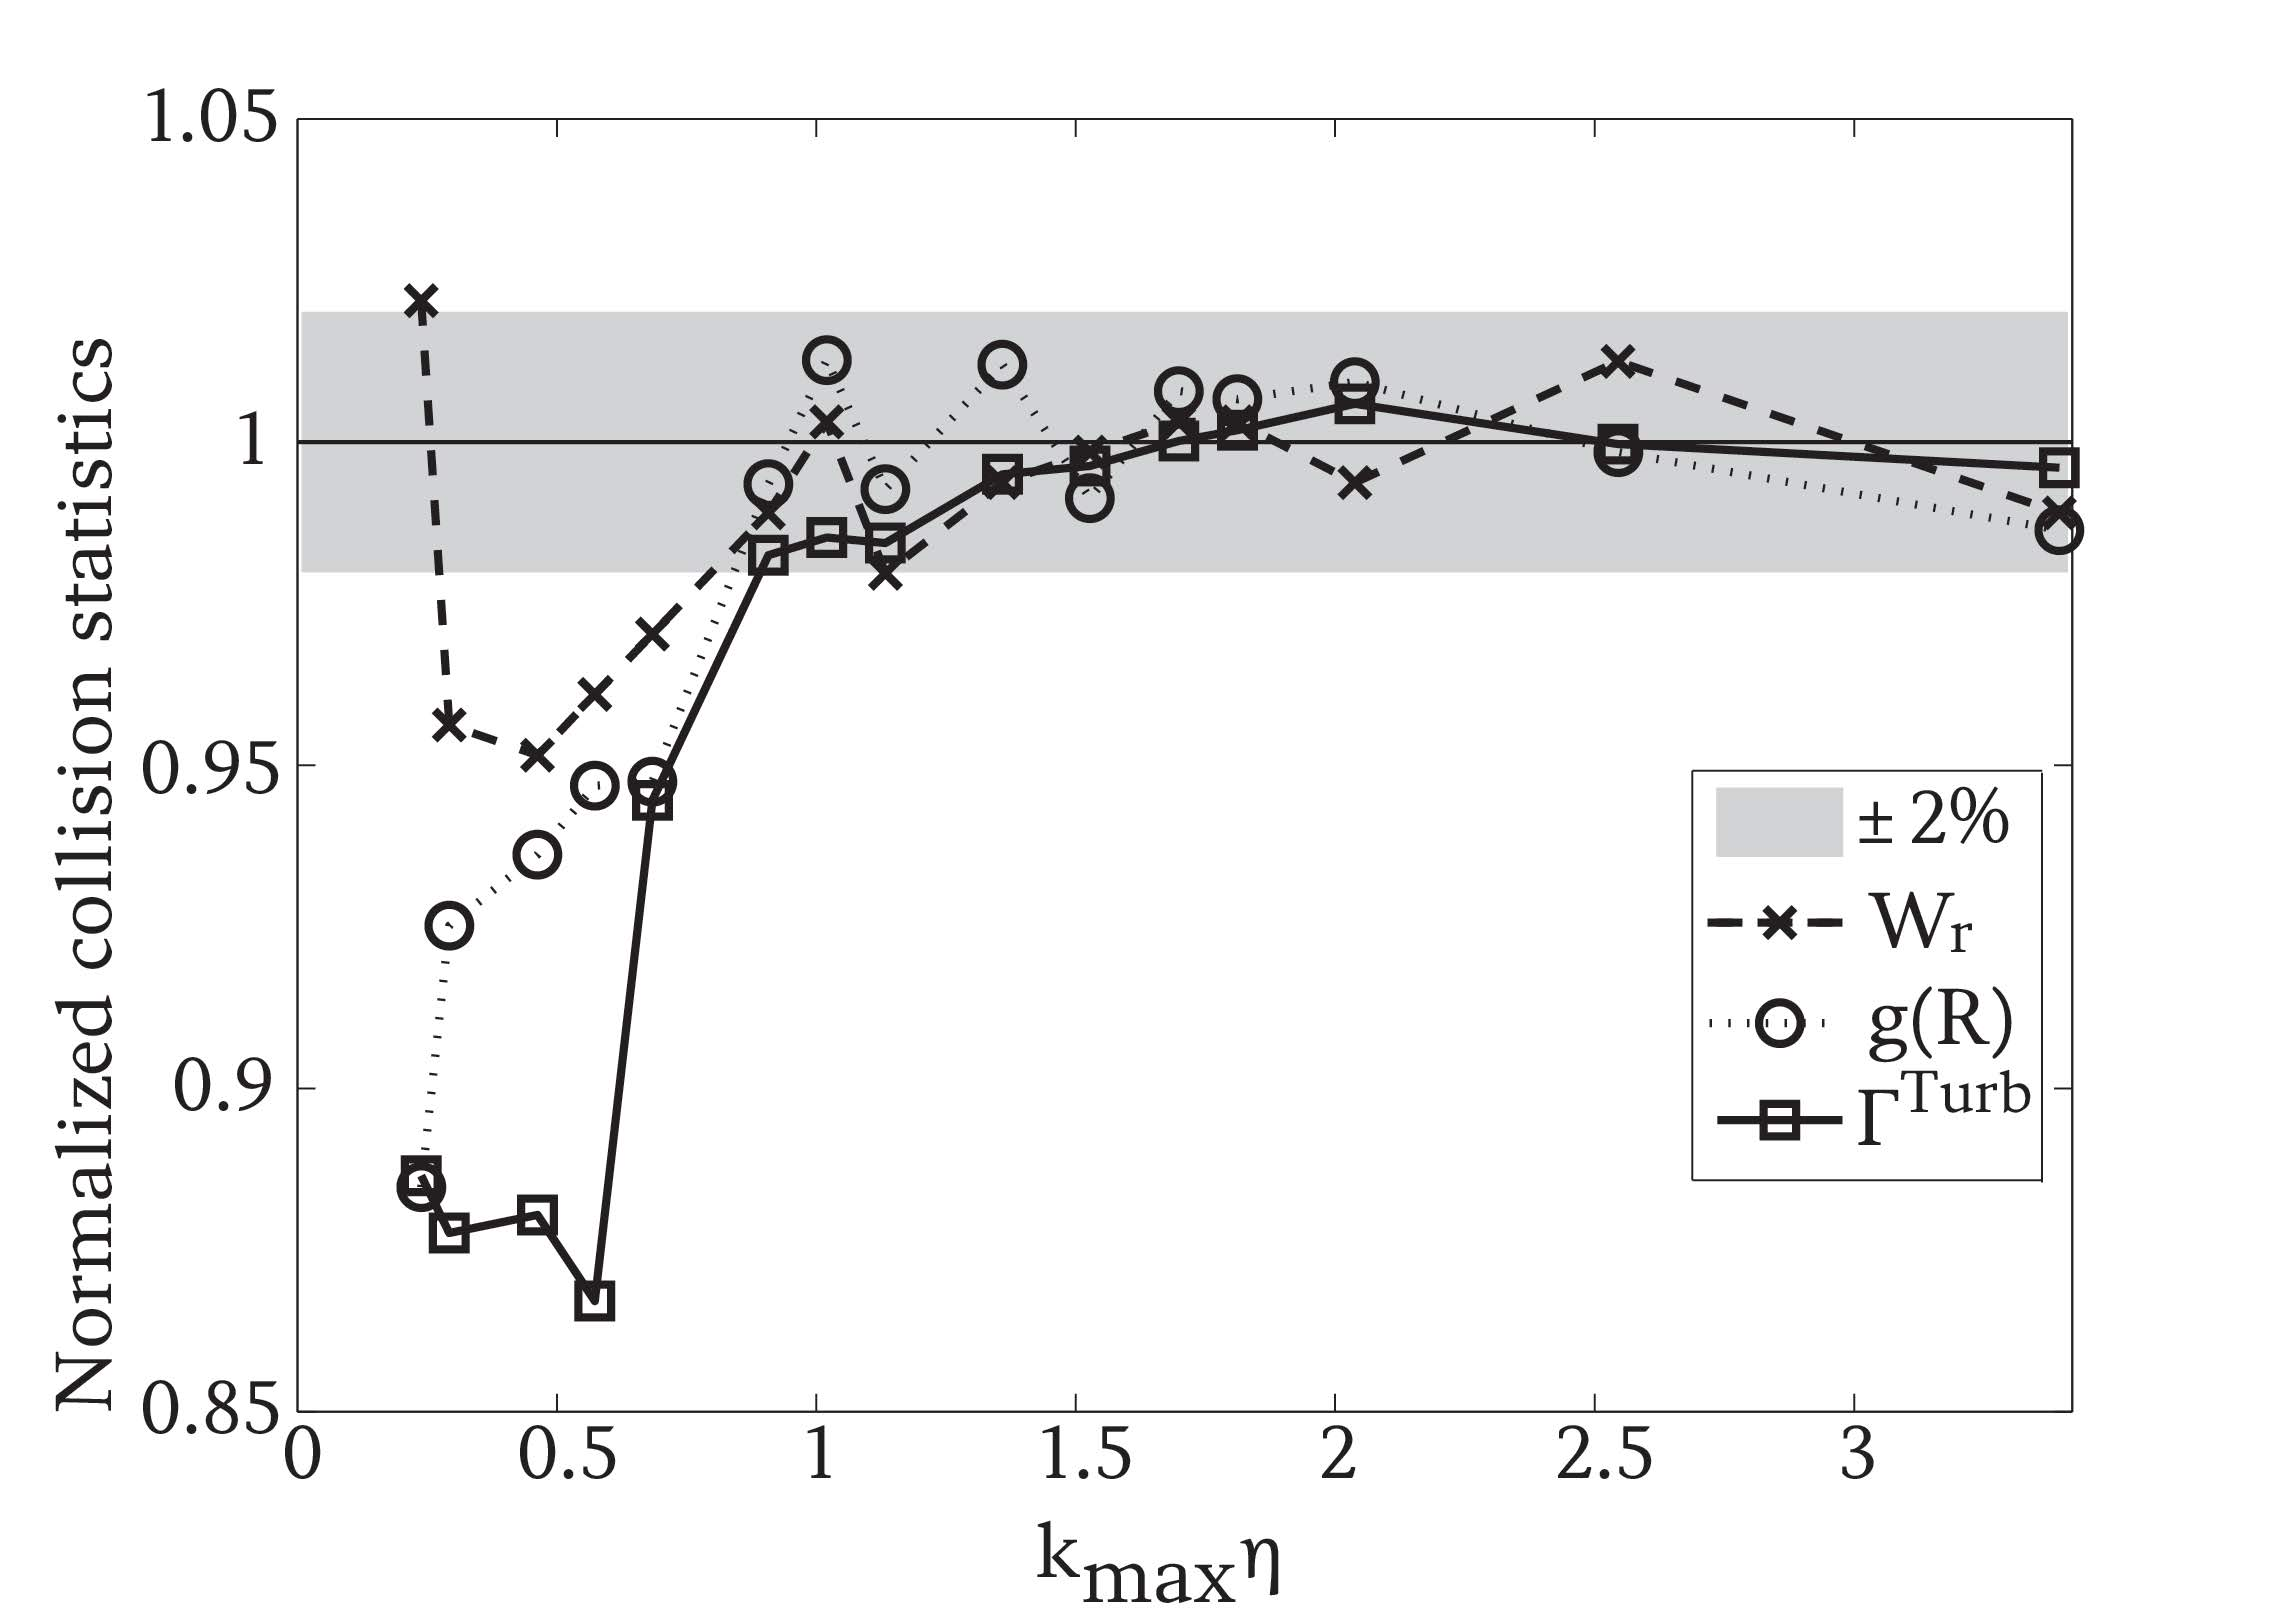
\includegraphics[width=\textwidth]{Figures/Chap2/kmaxeta.jpg} 
\caption{Collision statistics as a function of $k_{max}\eta$. All values are normalized by their respective average after $k_{max}\eta>1$. }\label{fig:kmaxeta1}
\end{figure}

To test the scalability of the code, we performed seven groups of simulations with different numbers of processors (2, 4, 8, 16, 32, 64, 128) on two different machines: The SGI Altix 4700 supercomputer at the University of Montreal and the Mammouth-parallel II machine at the University of Sherbrooke. Each group contained three members and we took the average of the three as a reference walltime. All tests were performed at $N = 256^3$ with $L=0.2$ m and we injected a total of $424,448$ droplets into the flow, half of which have a radius of 10 $\mu m$ and the other half with 20 $\mu m$. The code scales reasonably well on both machines. According to Amdahl's law, the performance of a parallelized program is constrained by its sequential part when number of processors increases \citep{Amdahl1967}. If the code is fully parallelized, the true walltime ($T_w$) will be half when number of processors ($N_p$) doubles. In other words, their relation can be precisely described by a power law formula with the power equals -1: $T_w=T_s\times N_p^{-1}$. Here $T_s$ is the walltime when the program is executed with single processor. The walltimes of our executions spanned from 60 minutes (with 128 processors) up to 2000 minutes (with 2 processors) on the SGI Altix, fitted into the curve of $T_w=3976$ (min) $\times N_p^{-0.8783}$. The experiments on the mp2 gave a fitted curve of $T_w=2433$ (min) $\times N_p^{-0.702}$. Even though we did not attain perfect scalability on both machines, we saw a significant speed-up of the simulations as the number of processors doubled. 

\subsubsection{Improvements in computing statistics of flow parameters} \label{sec:ch2_flowpara}

In this paper we used different approaches to obtain the EDR, the Taylor micro-scale ($\lambda$), and the $R_\lambda$ of the flow field. \citet{Franklin2005} estimated EDR from the energy spectrum, while we calculated it from the numerical integration of enstrophy ($\epsilon = 2\nu Z$, where Z is the total enstrophy), which provides more accurate values. $\lambda$ was calculated via $\sqrt{\frac{KE}{Z}}$ in \citet{Franklin2005}, where $KE$ is the total kinetic energy in the system, and our $\lambda$ was from $\sqrt{\frac{15\nu u\prime^2}{\epsilon}}$. Here $u\prime=\sqrt{\frac{2(KE)}{3}}$. $R_\lambda$ in our study was computed via $\frac{u\prime\lambda }{\nu}$, while $R_\lambda = \frac{\lambda\sqrt{2(KE)} }{\nu}$ in \citet{Franklin2005}.  Of course, these quantities respect the same scaling in Kolmogorov phenomenology, but not with the same proportionality constants. 

To quantify the difference in the resulting flow statistics, we re-ran the four cases in \citet{Franklin2005}. The results are listed in table \ref{tab:comp1} along with the \citet{Franklin2005} results for comparison. N is the number of grid points, ke is the initial KE. Flow statistics show that $\lambda$ in our study was around 3.0 times the value in \citet{Franklin2005} and $R_\lambda$ around 1.85 times. Since we did not change the actual properties of the flow but only the method of evaluating these statistics, similar collision statistics were expected under the same particle tracking and collision detection techniques. Indeed, the collision statistics in table \ref{tab:comp1} show that our results were indeed close to those of \citet{Franklin2005}, within a difference of $11\%$.


\begin{sidewaystable}
\begin{center}
\def\arraystretch{1.5}
\caption{Statistical parameters of the turbulent flow fields and corresponding collision statistics of four simulations from our study and from \citet{Franklin2005} (denoted as F05)\strut} \label{tab:comp1}
\begin{tabular}{ccccccccc}
\hline\hline
 N & \multicolumn{2}{c}{ $80^3$} & \multicolumn{2}{c}{$120^3$} & \multicolumn{2}{c}{$180^3$} & \multicolumn{2}{c}{$240^3$} \\
\hline
 model & DNS-MPI  & F05 & DNS-MPI &  F05  & DNS-MPI & F05 & DNS-MPI & F05 \\
\hline 
\multicolumn{9}{c}{Statistical parameters of the turbulent flow fields}\\

$\epsilon$(cm$^2$ s$^{-3}$) & 155 & 95 & 544 & 280 & 1371 & 656 & 2710 & 1535 \\ 

$\lambda$ (cm) & 1.10 & 0.35 & 0.90 & 0.29 & 0.78 & 0.26 & 0.70 & 0.23 \\ 
 
$R_\lambda$ & 60 & 33 & 76 & 40 & 89 & 48 & 102 & 55 \\ 

$u\prime$(cm s$^{-1}$)& 9 & 9 & 13 & 12 & 18 & 16 & 23 & 21 \\ 

$k_{max}\eta$ & 1.8 & 1.8 & 2.0 & 2.1 & 2.4 & 2.6 & 2.7 & 2.7 \\ 
 
$\eta (cm)$ & 0.07 & 0.07 & 0.05 & 0.06 & 0.04 & 0.05 & 0.04 & 0.04 \\ 
\hline
\multicolumn{9}{c}{Collision statistics}\\

$\Gamma \times10^{10}$ ($m^3 s^{-1}$)  &   $1.1267$  & $1.1054$ & $1.2940$  & $1.2420$  & $1.6629$ & $1.4960$  & $2.2736$ &  $2.1748$ \\ 

$g(R)$ & $1.0779$ & $1.0825$  & $1.1329$  & $1.1621$ & $1.2847$  & $1.2432$ & $1.4720$ & $1.4183$  \\ 
$\mathbf{W_r}$ (cm s$^{-1}$) & $1.85$  &  $1.8650$  &  $2.00$  & $2.1248$  & $2.26$   & $2.1248$  & $2.76$ & $2.7518$ \\

\hline 
\end{tabular} 
\end{center}
\end{sidewaystable}

\subsubsection{Separating the effects of $R_\lambda$ and EDR} \label{sec:ch2_separate}

As explained in section \ref{sec:ch2_intro}, the conclusions regarding $R_\lambda$ from \citet{Franklin2005} needs further exploration since the effects of EDR and $R_\lambda$ cannot be separated. To solve this problem we fix $\Delta x$ when simulating the same EDR, since EDR is determined by $\Delta x$ alone when $k_{max}\eta$ is fixed (See section \ref{sec:ch2_compares}). To increase $R_\lambda$, we increase the number of grid points (N) and hence the computational domain size (L), thereby resolving larger scales of the flow while keeping EDR fixed. Since $\Delta x$ in our study is linearly proportional to $\eta$ and $R_\lambda$ scales with domain size, L, it follows that $N \equiv L/\Delta x \propto L/\eta \propto (R_\lambda)^{3/2}$. Therefore, when varying $R_\lambda$ at fixed EDR, we changed N and fixed $\Delta x$. Likewise, when varying EDR to study its influence, we tuned $\Delta x$ to obtain our fixed value $k_{max} \eta=1.3$ and fixed N. 

\subsubsection{Two forcing schemes}\label{sec:ch2_forcing}

The total kinetic energy in the forcing band is fixed in \citet{Franklin2005}. We refer to this forcing scheme as forcing1. However, not knowing how much kinetic energy should be fixed to reach a desired average EDR, we have to manually adjust the initial energy in the forced waveband by trial and error, which is very inefficient. For this reason, we propose a modified version of the forcing (termed forcing2), which injects equal amounts of energy into the forcing band at each time step. The energy supply at the forcing scales is balanced by dissipation at the viscous scales when turbulence reaches statistical stationarity. It follows that the rate of energy injection can  easily be determined by the EDR at the initial time step and held constant thereafter. In this way, we decrease the amount of computations by specifying a steady average EDR directly.

To test the accuracy and efficiency of forcing2, we reran the simulation of \citet{Franklin2005} at $N=80^3$ with this forcing and compared the results with those from forcing1. The EDR for forcing1 was 155 $cm^2s^{-3}$ (see table \ref{tab:comp1}). We used this value to calculate the energy injection rate in the case of forcing2. Since the turbulence is both statistically stationary and ergodic, ensemble averages can be represented by time averaging.  Figure \ref{fig:specs} (a) demonstrates that forcing2 reproduced a very similar ensemble kinetic energy spectrum as forcing1 with a negligible difference of about 2\% in flow properties. This result demonstrates that forcing2 produces reliable results that are statistically identical to forcing1, but arrives at the kinetic energy spectrum, obtained by specifying the EDR, much more readily. To examine further the efficiency and accuracy of forcing2, we did another four simulations with $\epsilon \approx 1000 cm^2 s^{-3}$. The computational box size was fixed but resolution was different in each case. Figure \ref{fig:specs} (b) illustrates that the ensemble kinetic energy spectra from different resolutions lay on top of each other without any discernible shifts. This result lends support to the capability of forcing2 to produce precise mean EDR covering a range of spatial resolutions, since DNS average EDRs vary within only $\pm 1\%$. Although forcing2 is more efficient in controlling the average EDR than forcing1, most of our computations were obtained using forcing1. To avoid repeating the costly calculations our statistics will be analyzed from these data, bearing in mind that the EDRs show scatter within $\pm15\%$ from the desired value, but there were only two cases with scatter beyond $\pm10\%$. Forcing2 was used for the validation tests only.

\begin{figure}[ht]
\centering
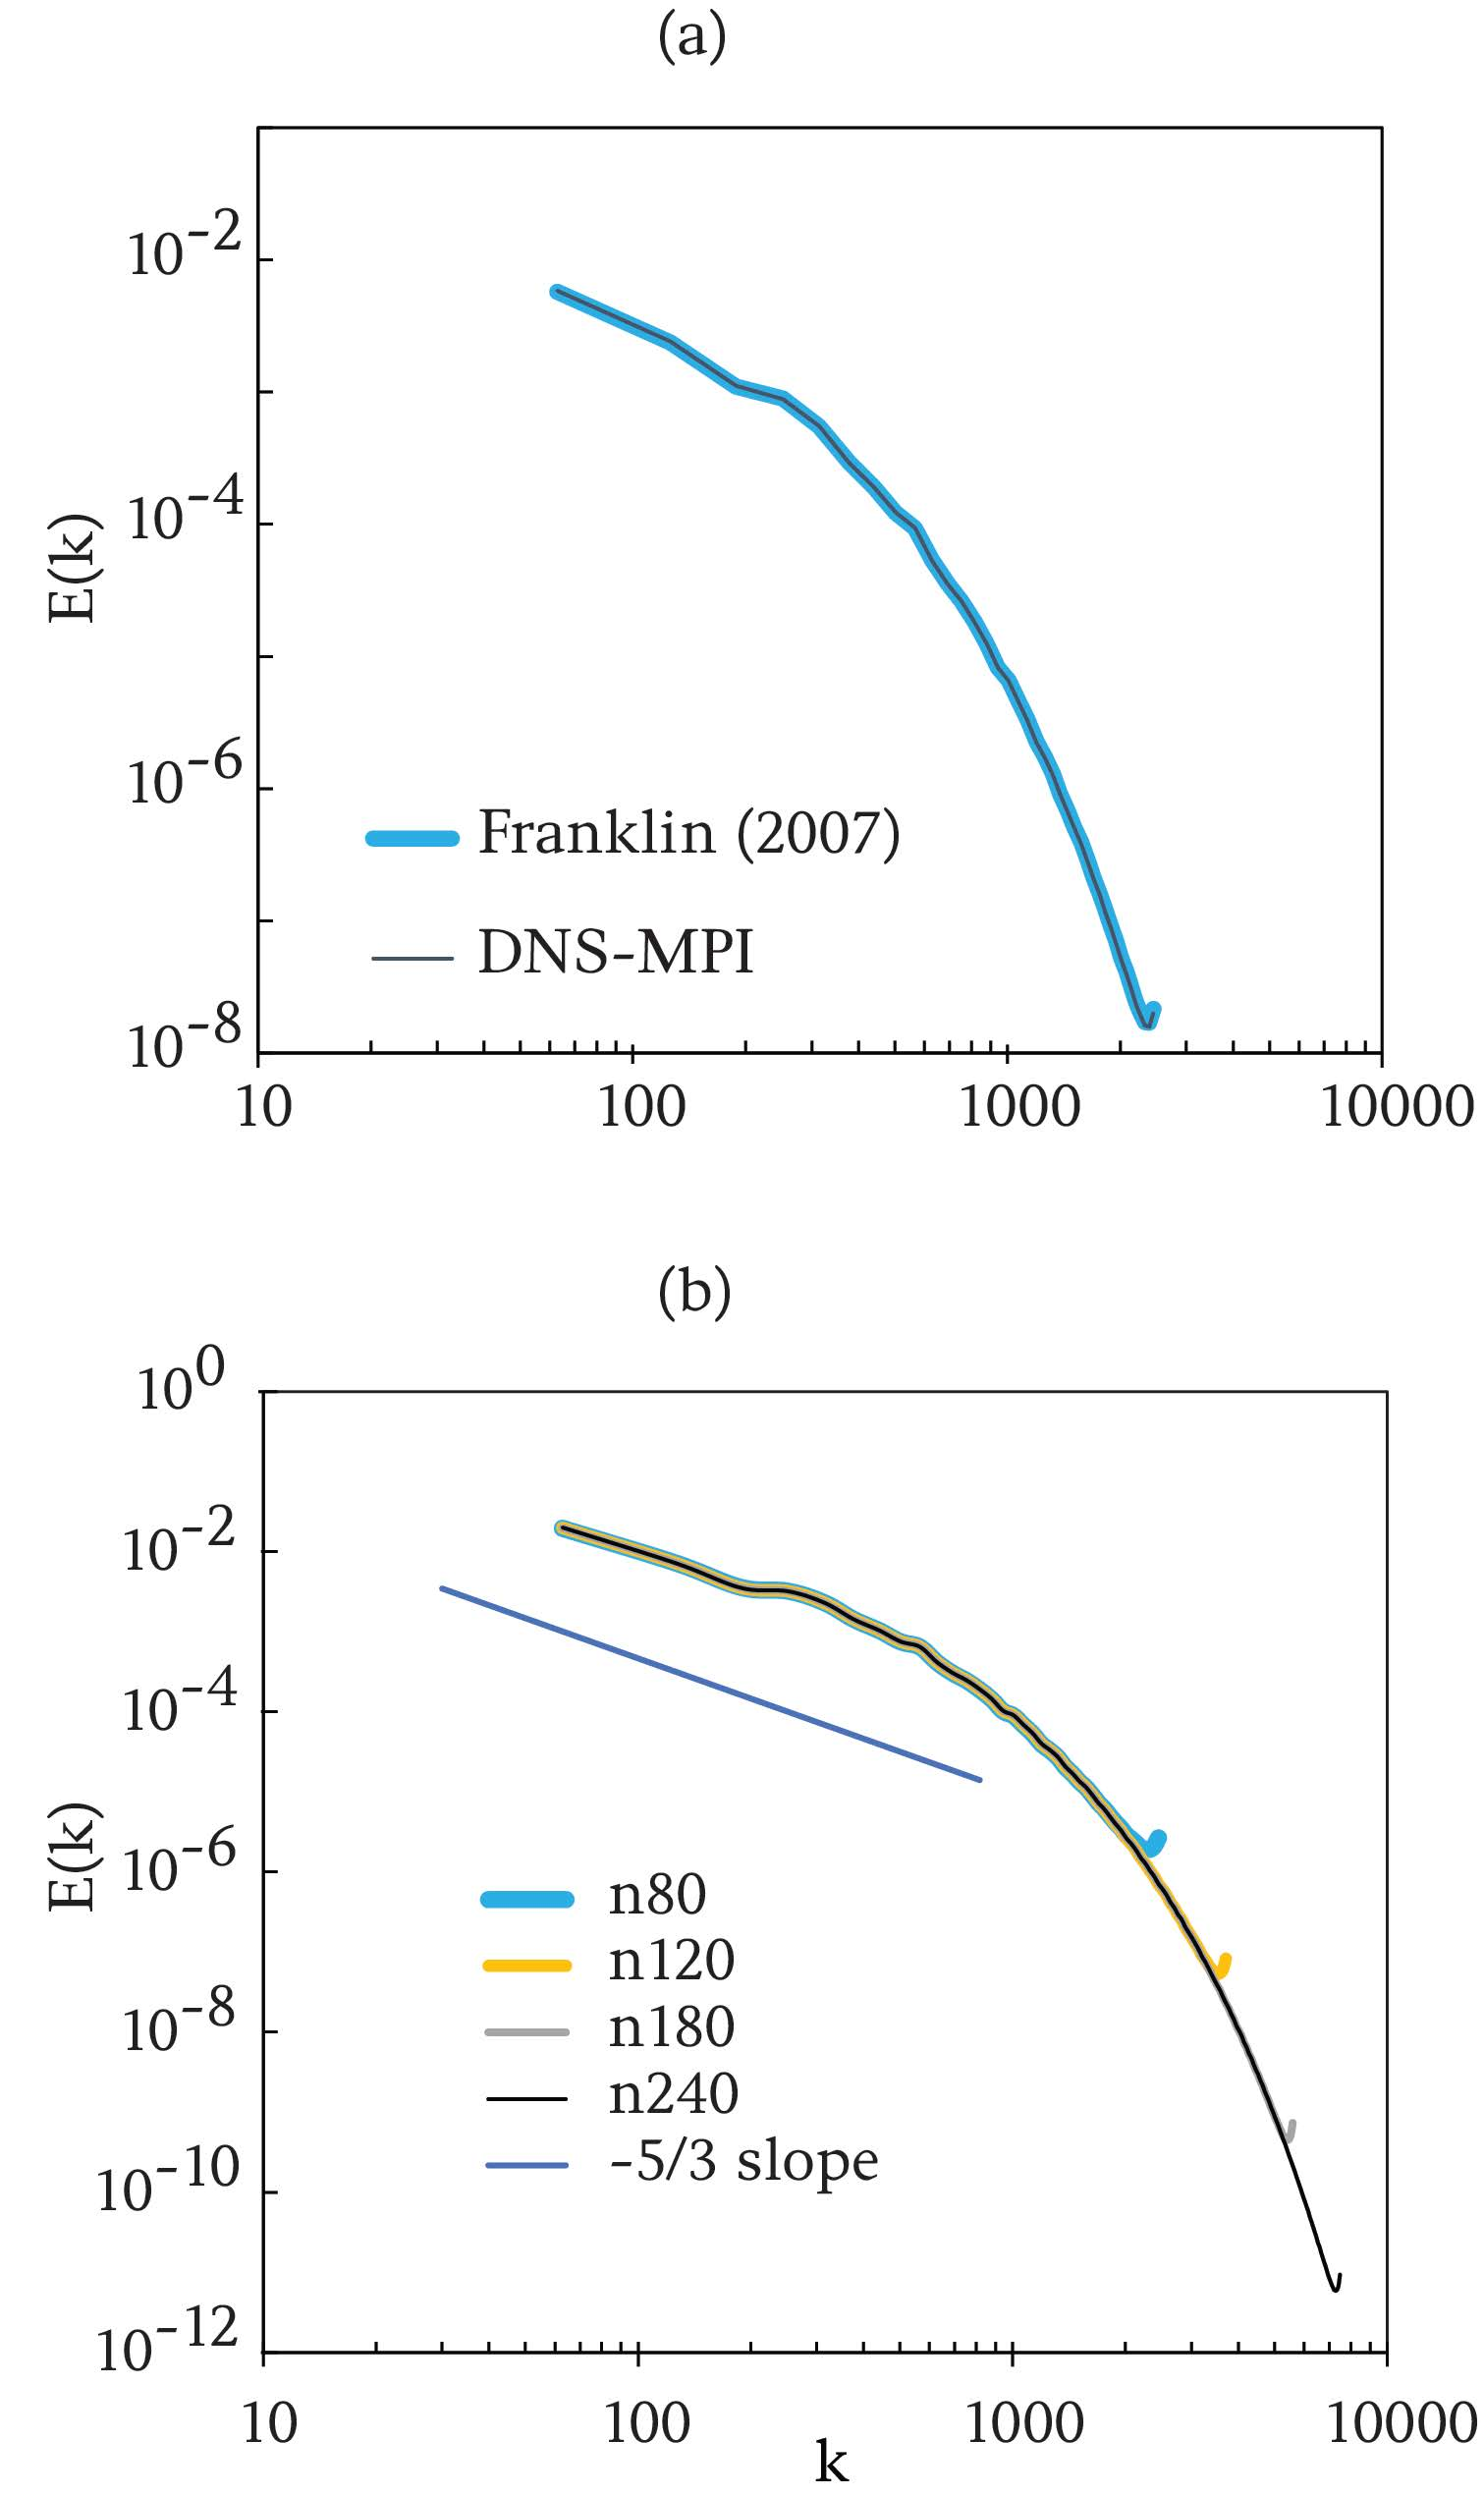
\includegraphics[width=0.7\textwidth]{Figures/Chap2/specs.jpg}
\caption{(a) Ensemble energy spectra from \citet{Franklin2007}'s forcing scheme (thick blue line) and from forcing2 (thin black line) with $\epsilon \approx$ 155 $cm^2s^{-3}$ and (b) ensemble energy spectra from forcing2 at four different resolutions with $\epsilon \approx 1000$ $cm^2 s^{-3}$, the domain width is fixed to 0.1 m in three directions for all simulations} \label{fig:specs}
\end{figure}

\section{Results} \label{sec:ch2_result}

To test the $R_\lambda$-dependency and EDR-dependency, our simulations employed five different eddy dissipation rates ($\epsilon = $ 50, 200, 500, 1000 and 1500 $cm^2s^{-3}$), and nine different box sizes ($N = 64^3, 96^3, 128^3, 192^3, 256^3, 384^3, 512^3$ and $1024^3$). We managed to run most of the scenarios except those with both high resolution and low dissipation rates (See figure \ref{fig:perform}). The reason is that N is largest in the highest resolution simulation and $\Delta x$ is largest at the lowest EDR run (see section \ref{sec:ch2_mpi})). As a consequence, the slab volume and the number of droplets assigned to each processor become very large, causing an inordinate amount of communication between processors yielding extremely slow computations. Nevertheless, the successful runs were sufficient for us to quantify the turbulence effects on droplet collisions as they span a broad range of EDR and $R_\lambda$.

\begin{figure}[ht]
\centering
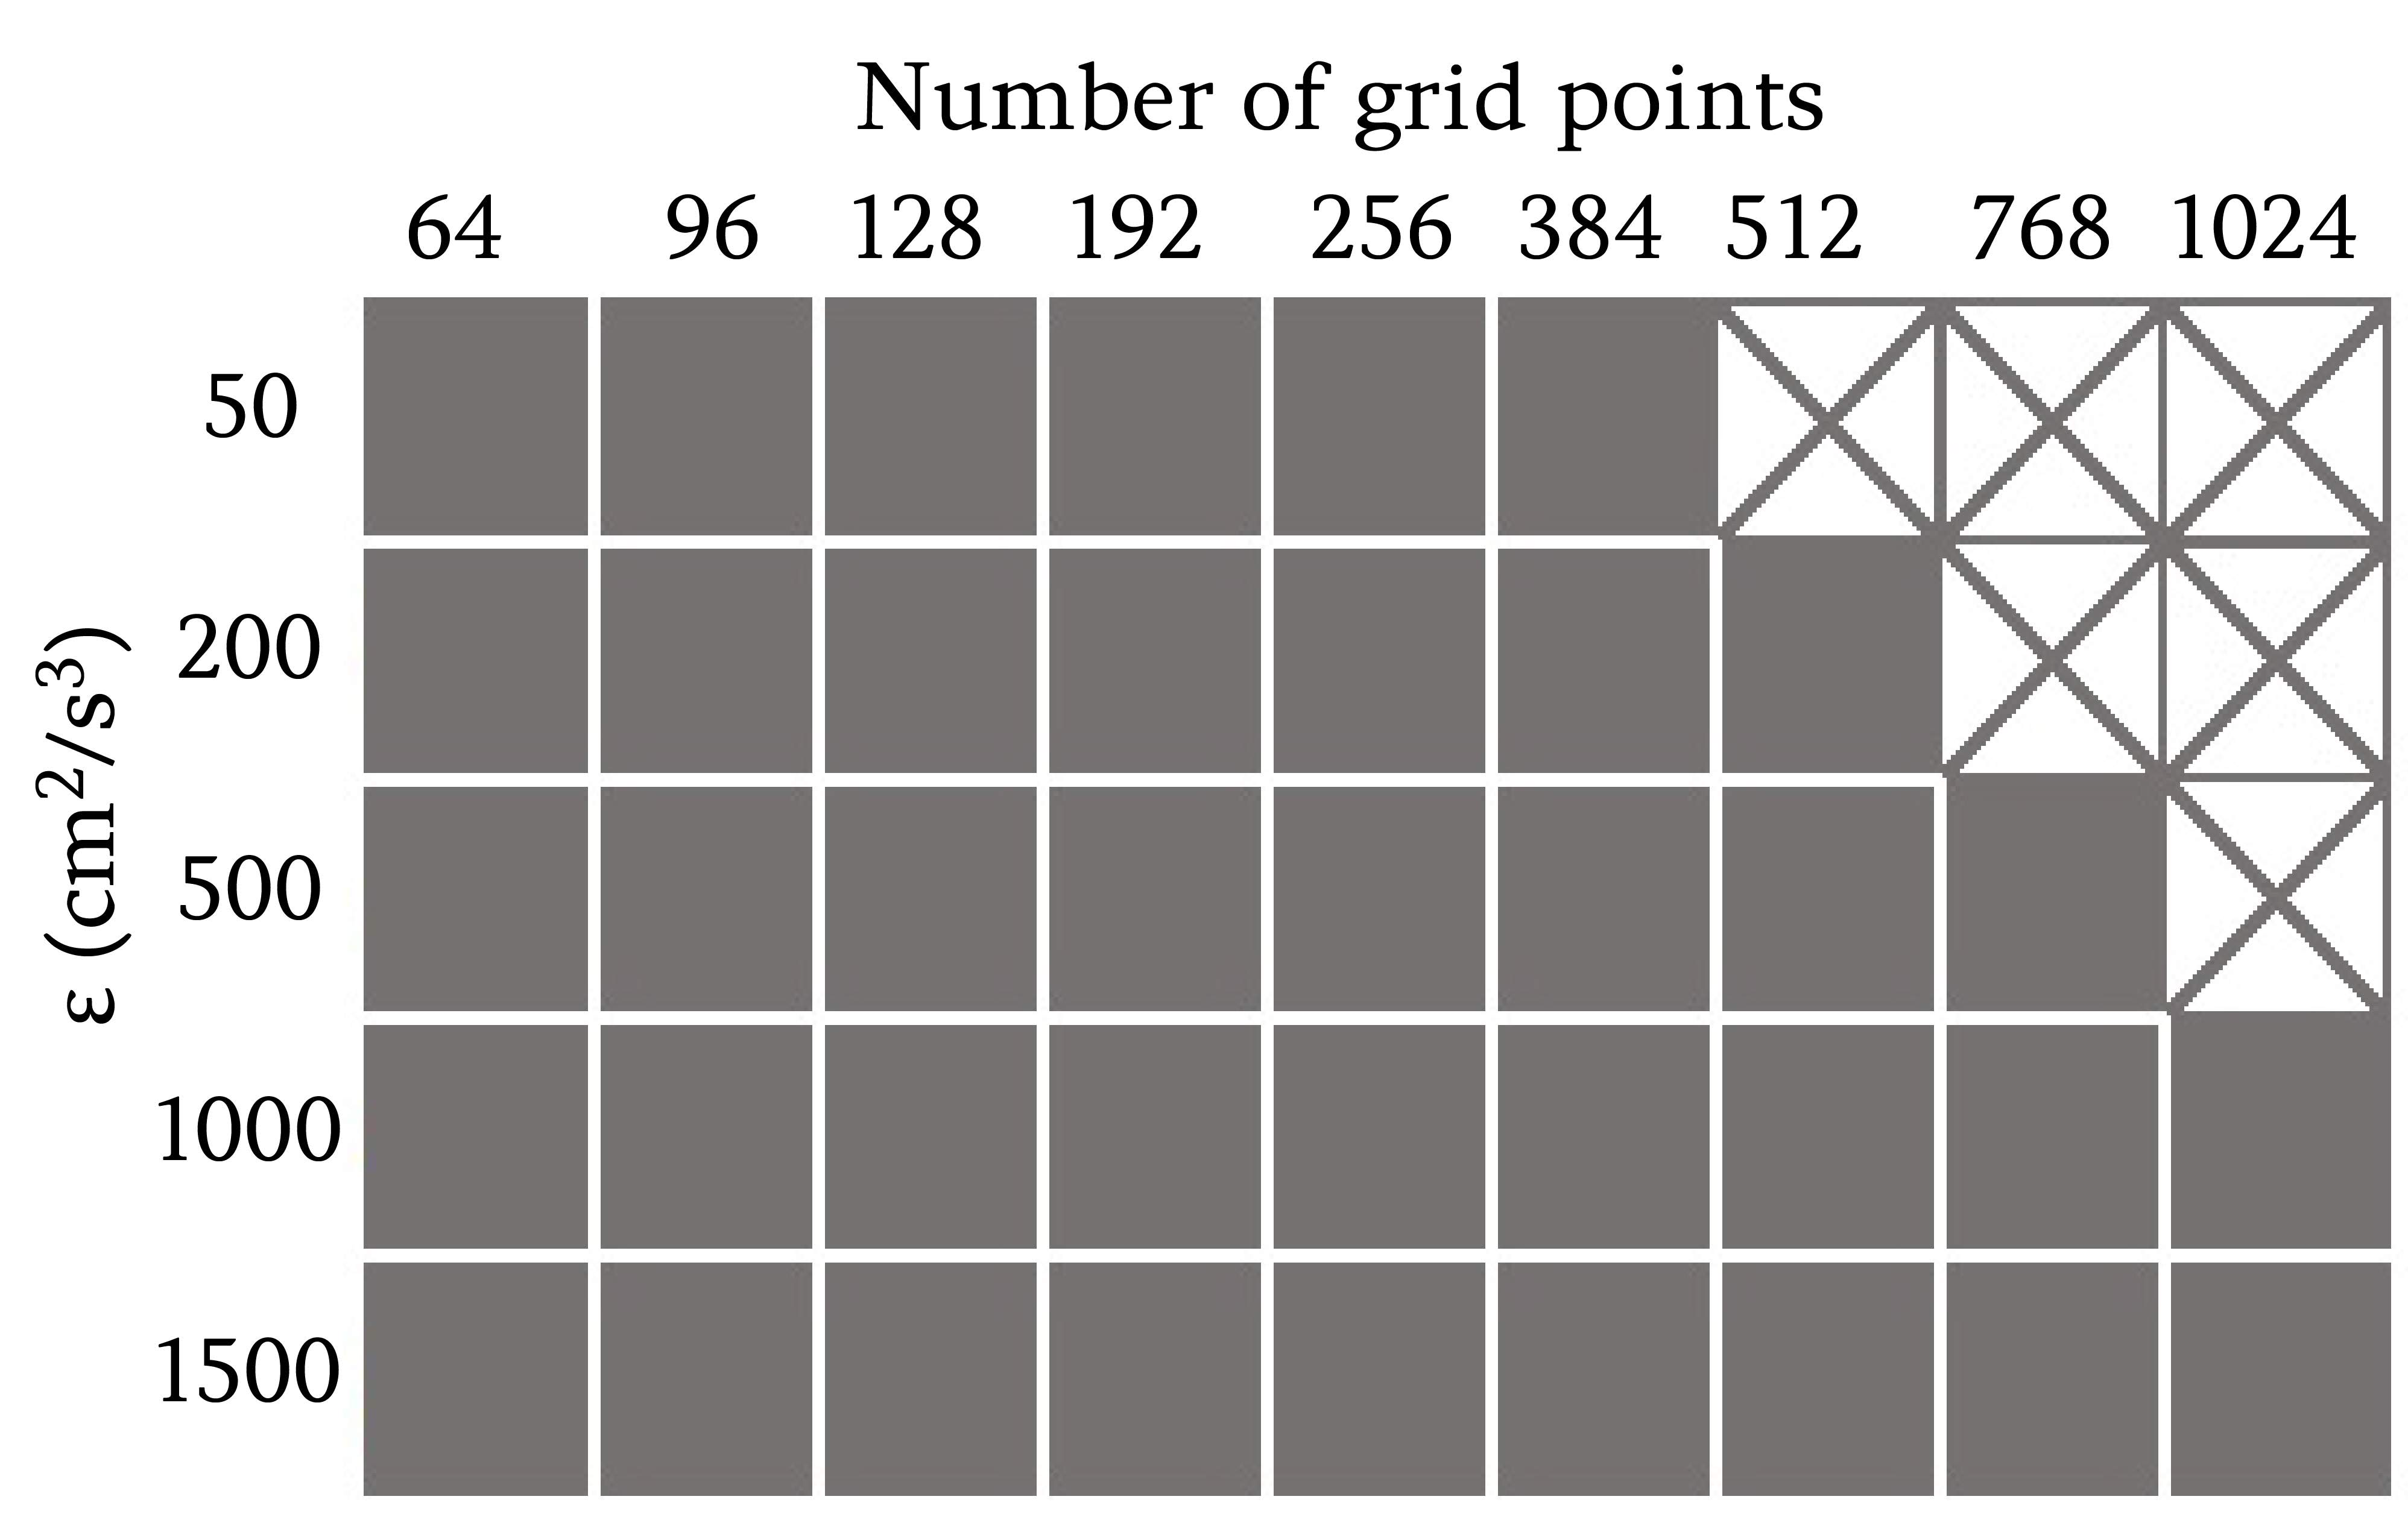
\includegraphics[width=0.8\textwidth]{Figures/Chap2/perform.jpg}
\caption {Overview of performed simulations over different $R_\lambda$-values and EDRs. Successful runs are shaded with gray, failed runs are marked by "$\times$"} \label{fig:perform}
\end{figure}


\subsection{Collision statistics with different box sizes ($R_\lambda$)} \label{sec:ch2_re}

The $R_\lambda$ in our simulations ranged from $63$ ($N=64^3$) to $589$ ($N=1024^3$), which gave us a good indication of how collision statistics depend on $R_\lambda$ or equivalently on the box size. \citet{Rosa2013} tested the convergence of collision statistics of 20-20 $\mu m$ droplet pairs and 30-30 $\mu m$ pairs with $R_\lambda$ using two different forcing schemes: one was stochastic forcing, where random acceleration was added to the velocity component in a low wave-number band, and the other was deterministic forcing in which the energy level in the two smallest wavenumber bands was fixed. They concluded that the RDF between large droplets ($r=30$ $\mu$m) were harder to converge with $R_\lambda$ than between small droplets ($r=20$ $\mu m$) because they were under the influence of larger scales of motion. The growing trend at low $R_\lambda$ in both forcings, as explained in their paper, was because more collision-related scales were resolved when $R_\lambda$ increased until a saturation level was reached. In addition, there was another possible contribution. Although the average dissipation rate was set to 400 $cm^2 s^{-3}$ in all cases, some variations were observed. The curves of RDFs follow closely the fluctuations of average EDR in both forcing schemes. Under stochastic forcing the EDR increased slightly with $R_\lambda$ \citep[see section 4.1 and figure 2 in][]{Rosa2013} while the corresponding RDFs were larger as well (see figure 15 in their paper). Under deterministic forcing the EDR reached its peak around $R_\lambda \approx 100-200$ and a similar pattern was also found in the RDFs at $r=30$ $\mu m$. 
According to our DNS, the sensitivity of the RDF of 25-25 $\mu m$ droplets to EDR (i.e., $\frac{\Delta g(R)}{\Delta \epsilon}$) was about $1.42 \times 10^{-2}$ $(cm^2 s^{-3})^{-1}$ for EDR around $500$ $cm^2 s^{-3}$, i.e., increasing $1 cm^2 s^{-3}$ in EDR will result in an increase of $1.42 \times 10^{-2}$ in g(R). This implies that a change of $100$ $cm^2s^{-3}$ in EDR will result in a change of 1.42 in the value of RDF, which is of the same order of magnitude as that of the RDF fluctuations in their large $R_\lambda$ regions. In section \ref{sec:ch2_diss}, we will show in detail that collision statistics are very sensitive to the EDR. 


We are in a position to compare the collision statistics with a wider range of $R_\lambda$ under fixed EDRs. Figure \ref{fig:Re_ck} demonstrates the collision kernel between 10 $\mu m$ droplets and 20 $\mu m$ droplets with different $R_\lambda$, with each curve indicating different EDRs when using forcing 1. The curves fluctuate mainly because the mean EDR in each run scattered within 15\% from the nominal value shown in the legend. The standard deviation of the statistics increases with $R_\lambda$, which can be induced by the intensified intermittency of the turbulence as domain size increases. \citet{Kolmogorov1962} conjectured that the variance of local (instantaneous) dissipation rate, $\epsilon\prime$, normalized by its square mean value scales with Reynolds number as follows: $\frac{\overline{\epsilon\prime^2}} {\overline{\epsilon\prime}^2} \sim \big(\frac{L}{\eta}\big)^\mu = R_\lambda^{\frac{3\mu}{2}}$, with the intermittent exponent $\mu = 0.25$ confirmed by later experiments and atmospheric observations \citep[e.g., ][]{Pope2000, Siebert2010}. Note that $\frac{\overline{\epsilon\prime^2 }} {\overline{\epsilon\prime}^2}$ is also the vorticity kurtosis K, and can be used to quantify the level of intermittency. We calculated K with different $R_\lambda$ at the EDR of $1000$ $cm^2s^{-3}$ and found our exponent consistent with $\mu=0.25$ with a relative error of 2.75\%. Though intermittency experienced a power law growth with the expansion of domain size, the collision kernel shown in figure \ref{fig:Re_ck} nevertheless is insensitive to $R_\lambda$, explicitly showing that the effect of intermittency is insignificant, at least over the simulated range. This flatness with $R_\lambda$ was also found in the collision kernel of all other droplet pairs including both same-sized collisions and cross-sized collisions as shown in panel A-B of figure \ref{fig:re_cs}. The standard deviation was of a similar order of magnitude as in figure \ref{fig:Re_ck} and therefore is not shown. The fluctuations in the curves were caused by slight variations in the dissipation rate, as mentioned earlier. As can be seen from the gray dashed line in panel A(ii), the EDR varied around $500$ $cm^2 s^{-3}$ over different simulations, creating a spike around $R_\lambda = 180$. This, as a consequence, diminished the flatness of these collision statistics. Panel B of the figure demonstrates the same fact with another dissipation rate. As for RDF and RRV shown in panel C and D respectively, the Reynolds number did not alter the collision statistics. Specifically, previous studies have shown that clustering happens in low-vorticity regions \citep[e.g., ][]{Maxey1987}. Therefore, we found it interesting that the RDF is also independent of domain size and we conclude that intermittency has a relatively small impact. However, this conclusion has to be interpreted cautiously. It is possible that the intermittency is still too weak, since the $R_\lambda$ here may not be sufficiently large to show the high levels expected in real cumulus clouds. The $R_\lambda$-independency implies that the large-scale motion has little effect on the droplets and the collision-related scales have been fully resolved at even small $R_\lambda$ ($\sim 60$). Droplets of small Stokes number adjust quickly to the local fluid acceleration before colliding with surrounding droplets and the local influence might greatly dominate over their acceleration history given by the large-scale motions. Thus, the effect, if any, of $R_\lambda$ on droplet collision statistics is secondary compared to the effects from the local dissipation rate and Stokes number. As discussed in section \ref{sec:ch2_intro}, the $R_\lambda$-dependency is in fact mainly the result of the model's inadequate flow scale separation seen only at very low resolutions, i.e., the failure to resolve all the collision-related scales is because the DNS box size is too small. Cloud systems are characterized by an enormous span of scales and their real Reynolds number is too large to be amenable to DNS. Thus the $R_\lambda$ calculated from DNS is determined by computational box size, L, rather than any real scale separation in clouds. The same conclusion can  apply to $u\prime$, following the scaling $u\prime = (\epsilon L)^{1/3}$. As a result, when interpreting the sensitivity of collision statistics to $R_\lambda$ from DNS data, we should be aware of the other quantities that are changing with the model configuration. We believe that the scale of turbulence affecting droplet collisions is on the order of the mean separation distance of cloud droplets. Generally, cloud droplet number concentration is on order of 10-1000 $cm^{-3}$, depending on the cloud type \citep[e.g., ][]{Twomey1959, Bennartz2007, Leaitch1992}. This gives an average droplet separation distance of the order of 0.1-1 mm, which is close to the order of the Kolmogorov length scale for the typical range of EDRs ($50-1500 cm^2s^{-3}$) in clouds. As long as the model resolves scales down to the droplet separation distance, which is far below our smallest computational domain size, $R_\lambda$ becomes irrelevant and the turbulence can be characterised by EDR alone. 


\begin{figure}[ht]
\centering
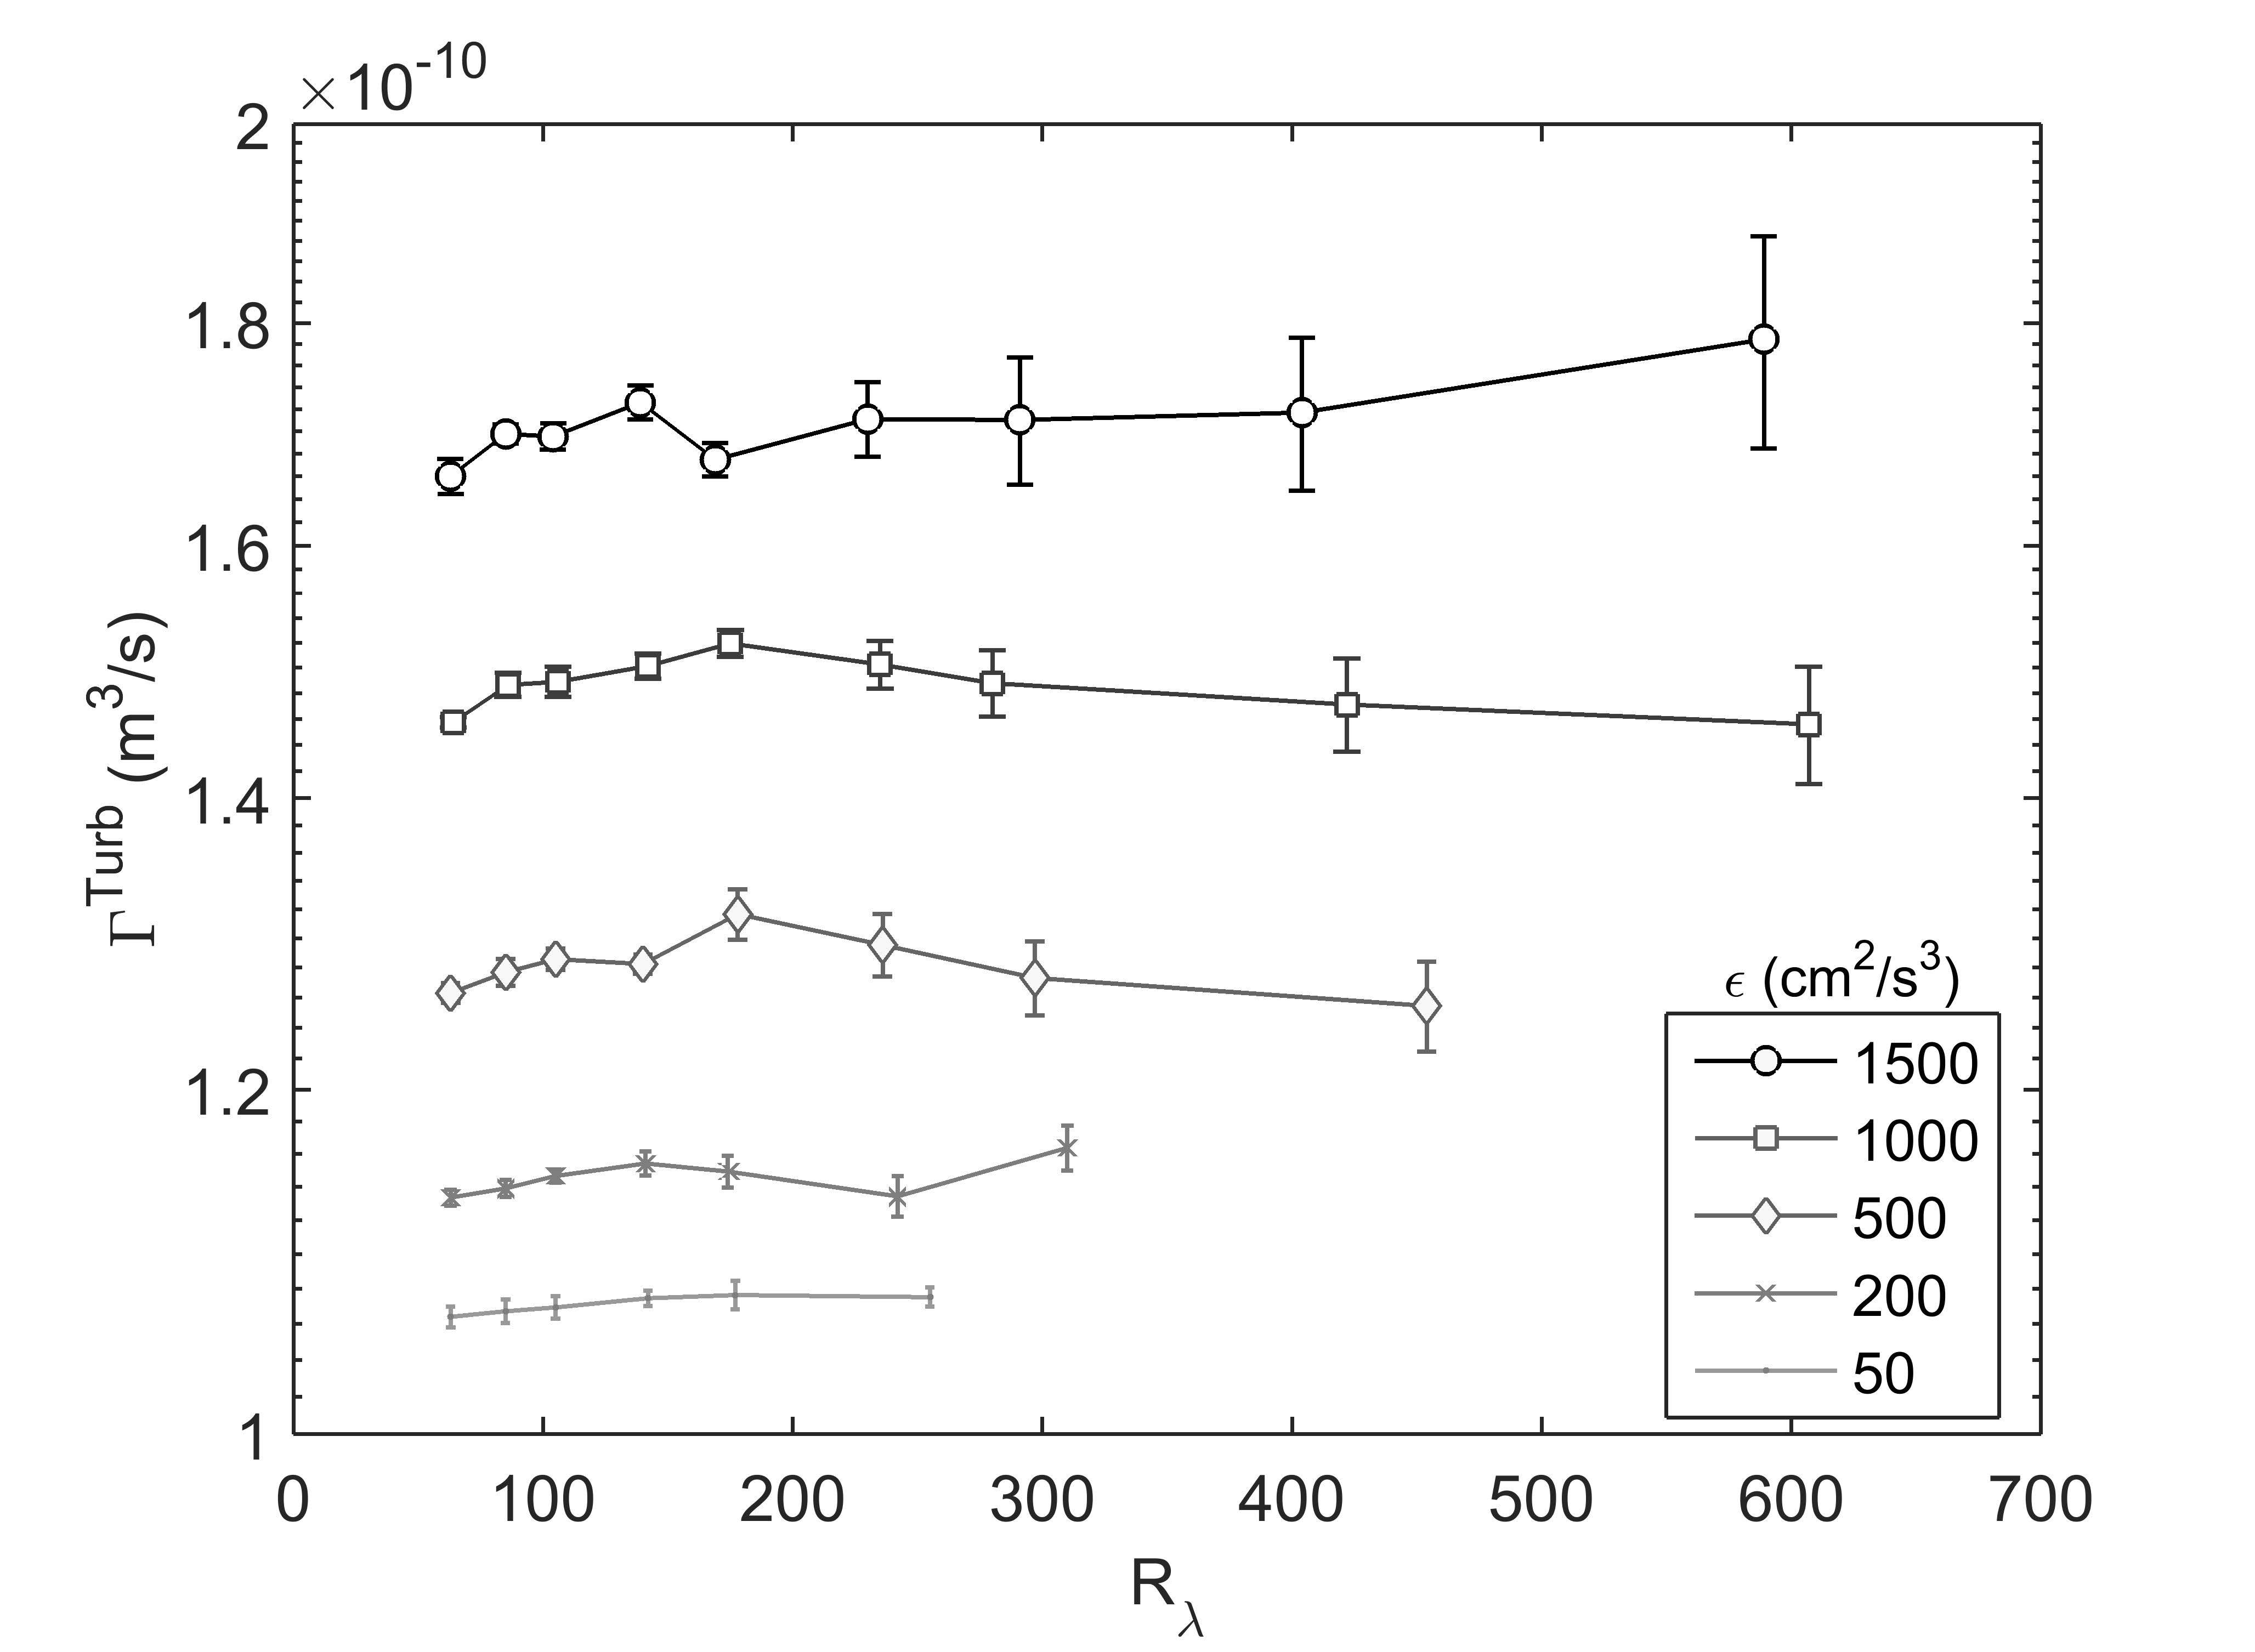
\includegraphics[width=0.8\textwidth]{Figures/Chap2/Re_ck.jpg}
\caption{Collision kernel of 10-20 $\mu$m collisions as a function of $R_\lambda$ with error bars representing one standard deviation. Values of EDR are represented by the grayscale.} \label{fig:Re_ck}
\end{figure}

\begin{figure}[ht]
\centering
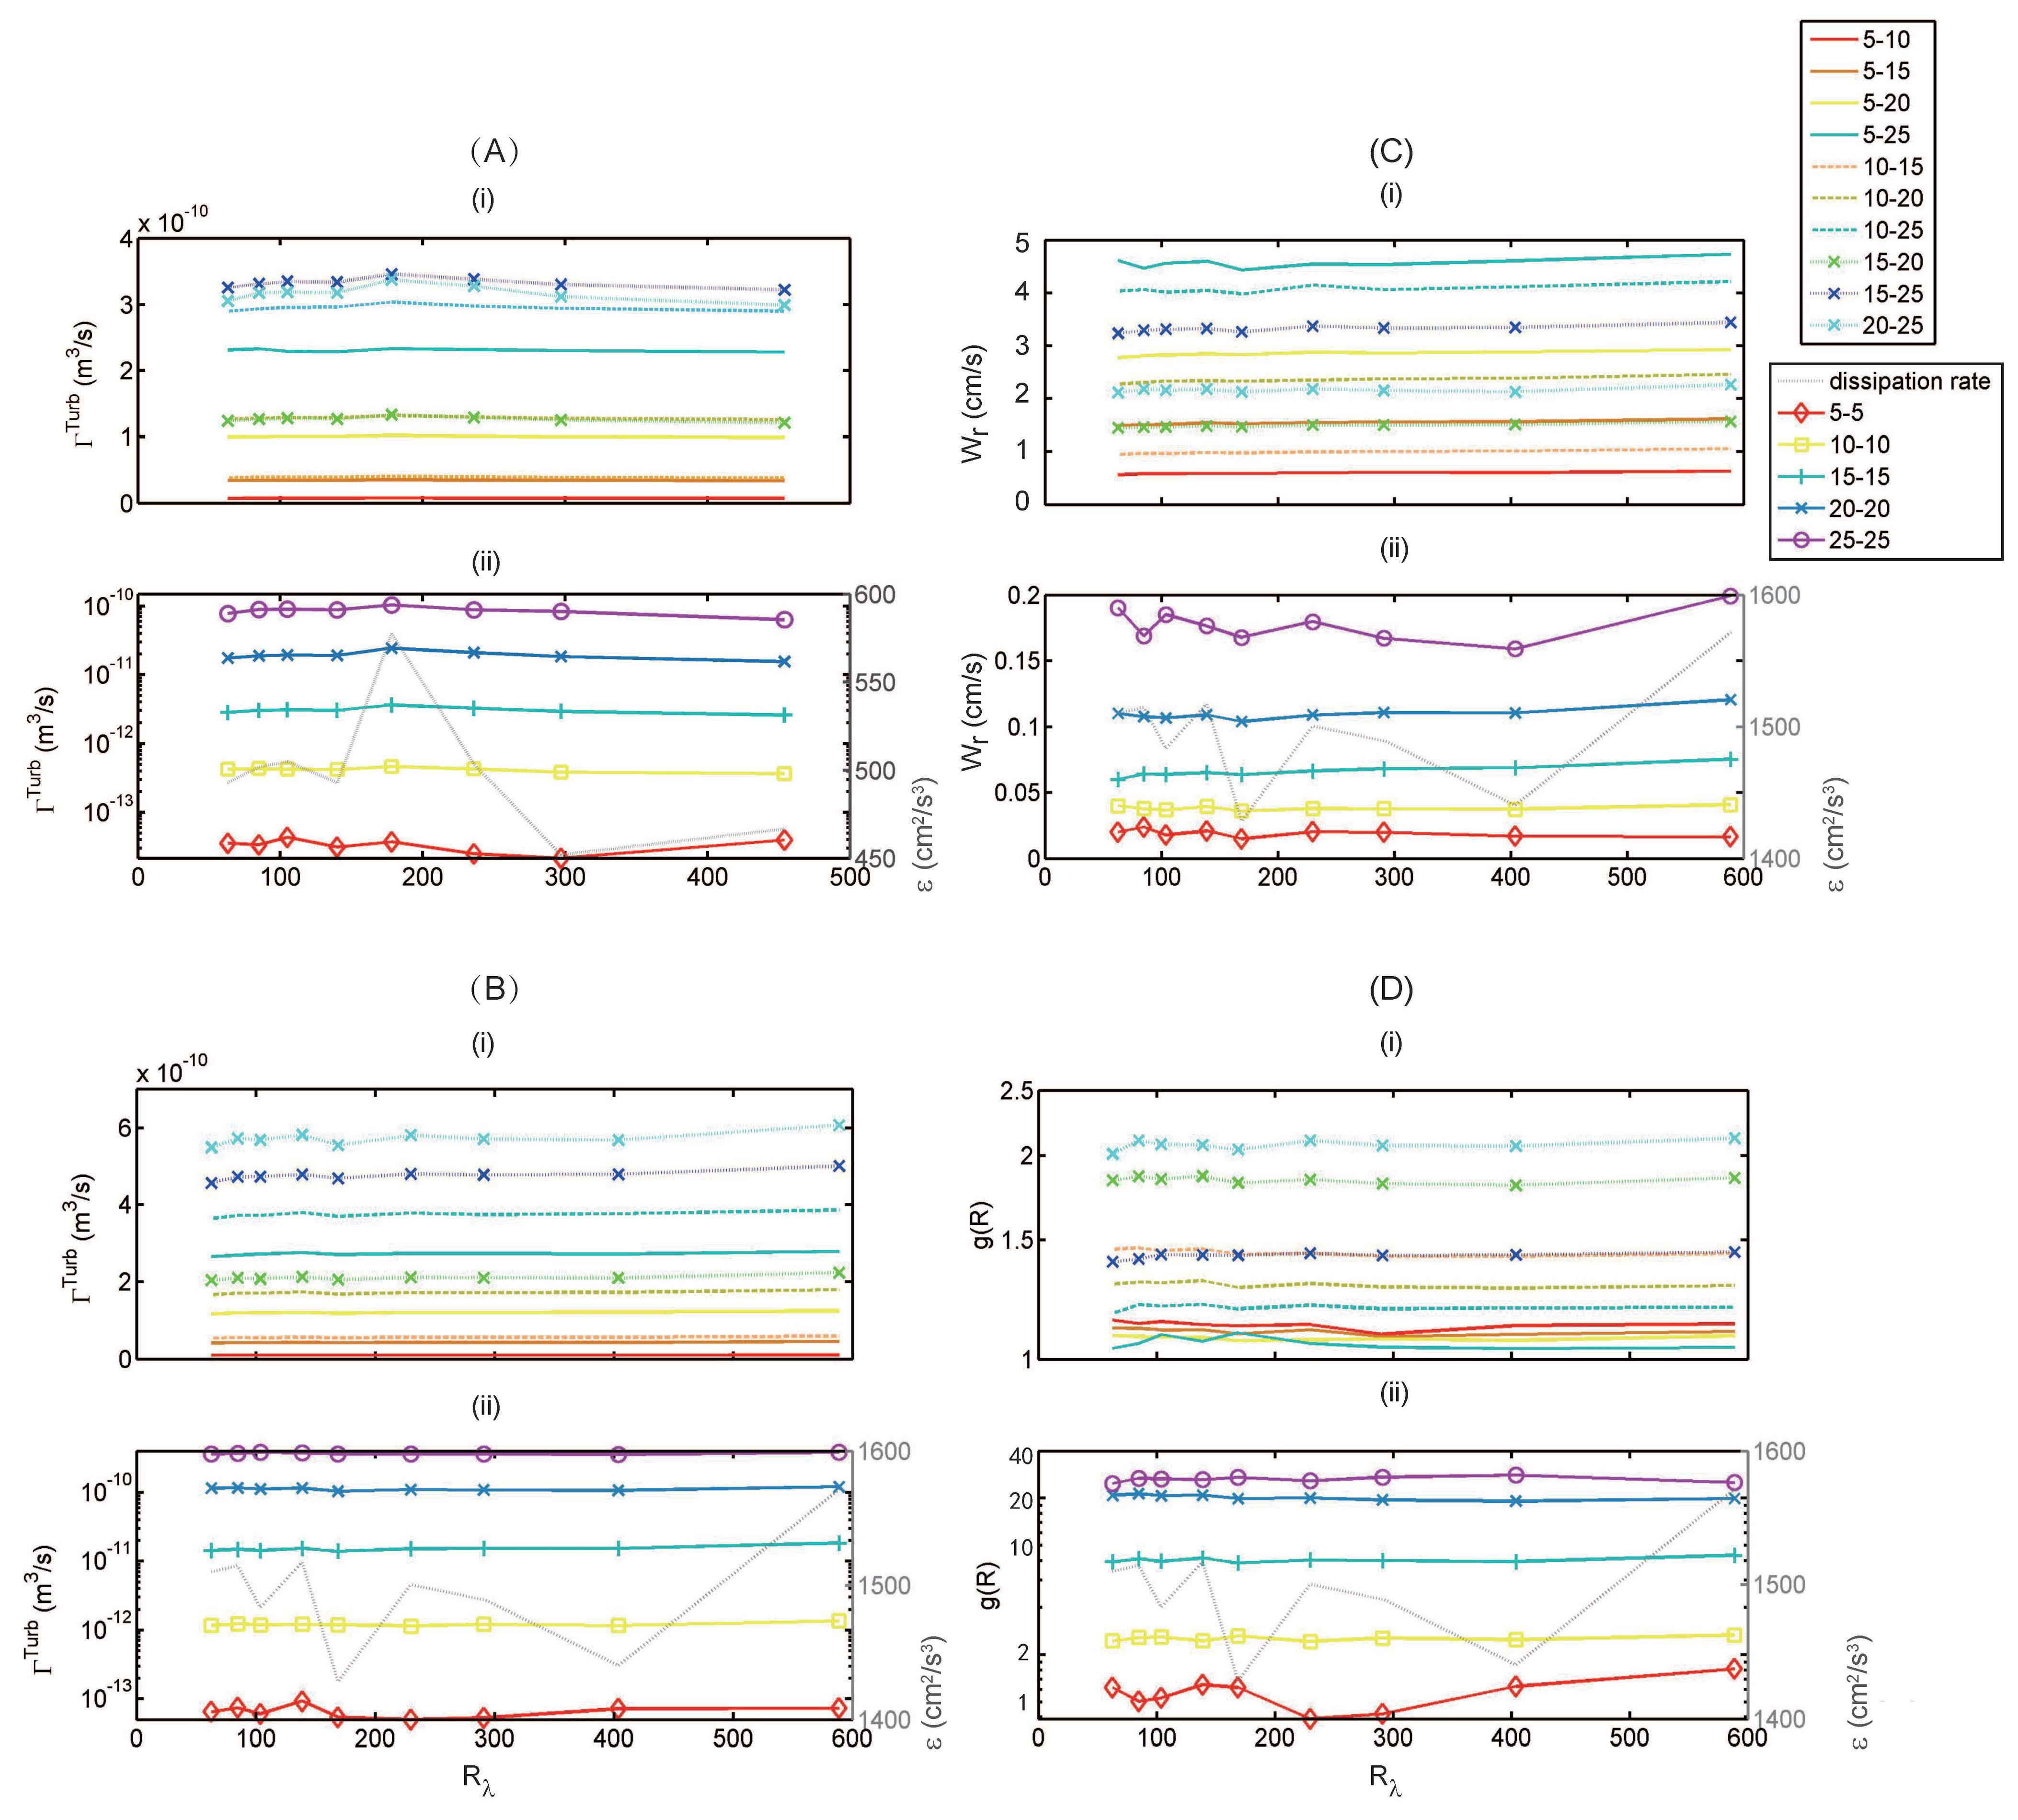
\includegraphics[width=\textwidth]{Figures/Chap2/re_cs.jpg}
\caption{ Collision statistics under different  $R_\lambda$ for all droplet pairs in this study. (A) and (B) are for collision kernels with $\epsilon \approx500$ cm$^2$ s$^{-3}$ and $\epsilon \approx1500$ cm$^2$ s$^{-3}$, respectively.  (C) and (D) are the same as (B) but for RRV and RDF, respectively. Results for cross-sized collisions are shown in (i)s and same-sized collisions in (ii)s. The gray dashed line depicts the EDRs under different simulations.} \label{fig:re_cs}
\end{figure}

\subsection{Collision statistics under different eddy dissipation rates} \label{sec:ch2_diss}

Since we have demonstrated that collision statistics are not sensitive to $R_\lambda$, we averaged over all resolutions in our studies to examine the effects of EDR. We found that all collision and pair statistics increase monotonically with EDR, which was consistent with the finding of \citet{Ayala2008a}. Among the three, RDF seemed to head towards an asymptotic value (figure \ref{fig:diss_cs} (b)).  The fluctuation of statistics among different resolutions grew slightly with increasing EDR, which can be attributed to the increasing intermittency of turbulence \citep[e.g. ][]{Pope2000}. 

\begin{figure}[ht]
\centering
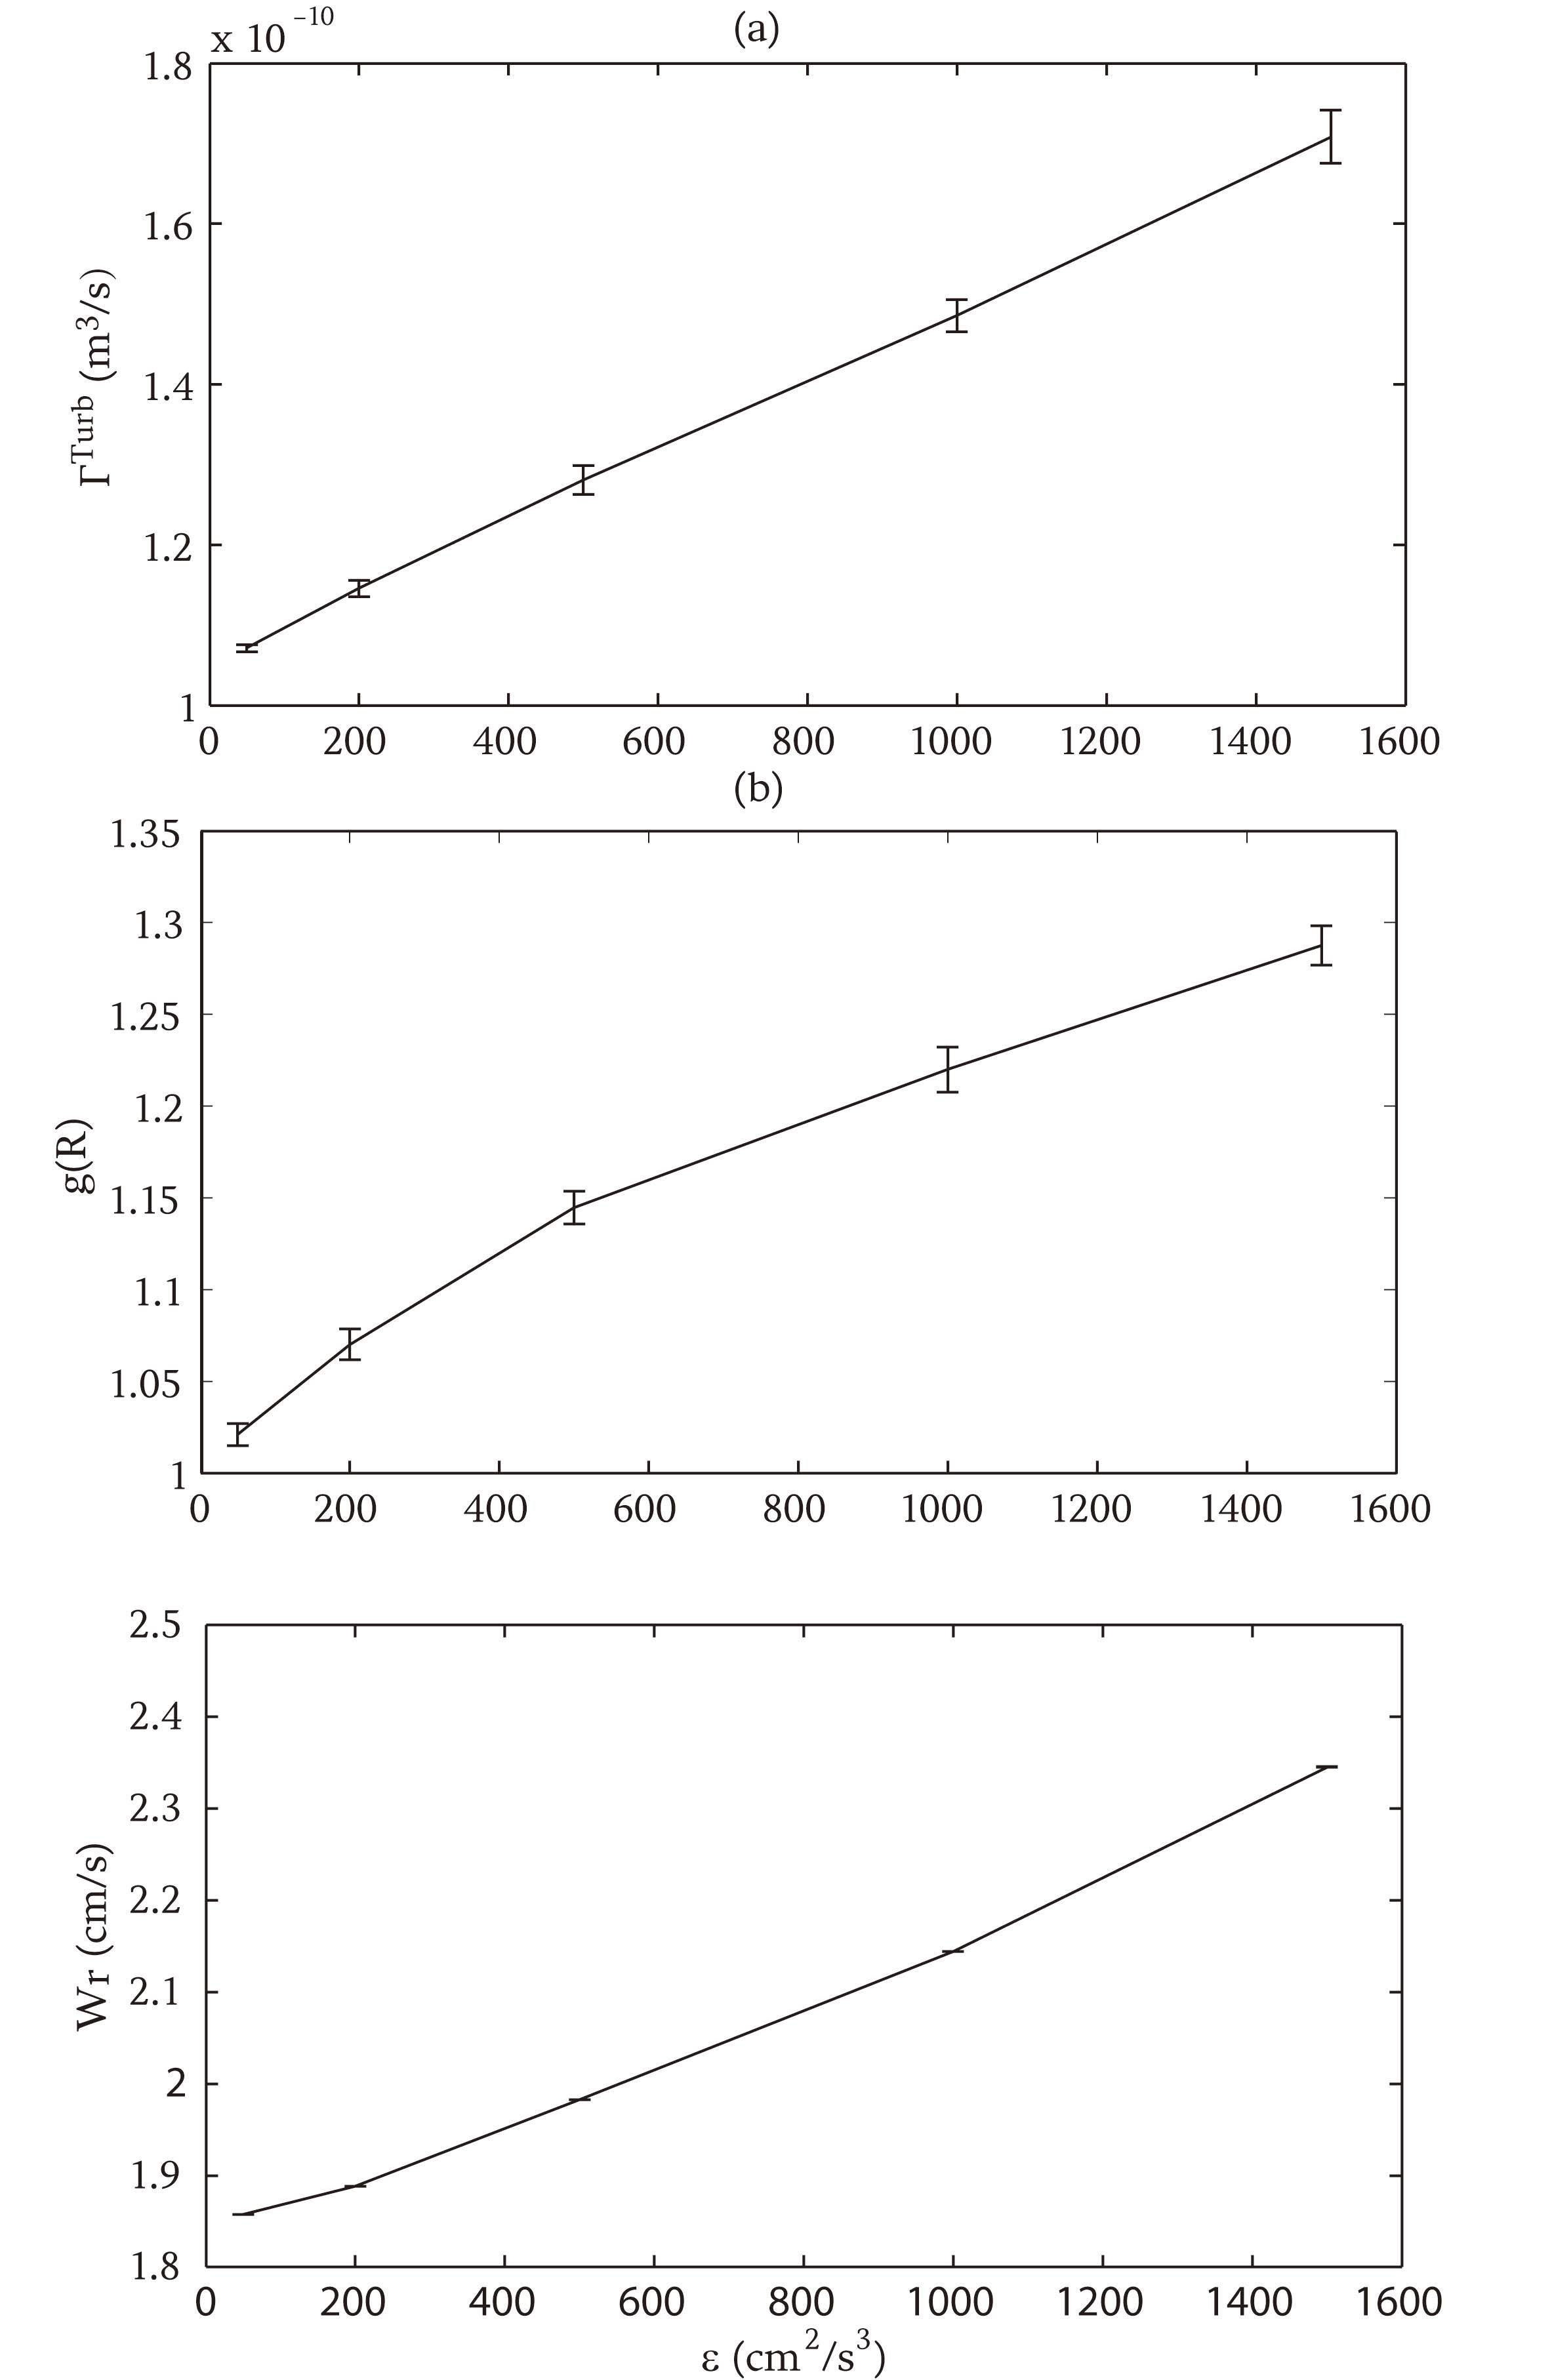
\includegraphics[width=0.8\textwidth]{Figures/Chap2/diss_cs.jpg} 
\caption{ Statistics of (a) collision Kernel, (b) RDF, and (c) RRV for droplets between 10 $\mu$m and 20 $\mu$m as a function of EDRs. The error bars show the standard deviation of the statistics with different $R_\lambda$-values} \label{fig:diss_cs}
\end{figure}

To better evaluate how EDR impacts the different droplet pairs, we normalized the statistics by their respective values in a purely gravitational setting. Since the results are insensitive to $R_\lambda$, or L, only simulations at one resolution  $N=256^3$ were examined. Figure \ref{fig:diss_cs_20_self} (a)-(c) showed that the cross-sized collision statistics involving 20 $\mu m$ droplets increased with EDR. The strongest enhancement in collision kernel occurs in the case of 20-25 $\mu$m droplet pairs, with a maximum enhancement of about 3.1 at the highest EDR. This increase was primarily attributed to the stronger clustering at high EDR, especially for the 20-25 $\mu$m droplet-pairs. Droplet pairs with similar size tended to cluster in the same regions of the flow due to similar droplet inertias and terminal velocities. This has been confirmed by previous studies \citep[e.g.,][]{Ayala2008a,Franklin2005}. An exception to this though, was pairs involving droplets with a radius $r = 5$ $\mu m$, that always seem to have a small value of RDF (see figure \ref{fig:diss_cs_20_self} (b)). This was probably due to the fact that small droplets have small Stokes numbers, indicating that they adjust very quickly to changes in the flow and therefore act more like fluid tracers than inertial droplets. The normalized RRV grew nearly linearly for all sizes with the strongest enhancement for 20-25 $\mu m$ pairs as well (figure \ref{fig:diss_cs_20_self} (c)). The results involving droplets of other sizes were similar and are thus not shown.

Same-sized collisions are impossible when gravity is the only influence on droplet motion because they have identical terminal velocities. However, when turbulence is present, collisions do occur. Before discussing the results it should be noted that there was a variation of about $3\%$ due to inadequate sampling, especially for droplets of $r=5$ $\mu m$ and 25 $\mu m$. The 5 $\mu m$ droplets had less chance to collide with one another due to their minute size and the 25 $\mu m$ droplets had the lowest concentrations among all the droplets, also leading to low collision rates. We can see from all panels of figure \ref{fig:diss_cs_20_self} that all three statistics increased with the size of droplet pairs, both for same-sized collisions and cross-sized collisions.

\begin{figure}[ht]
\centering
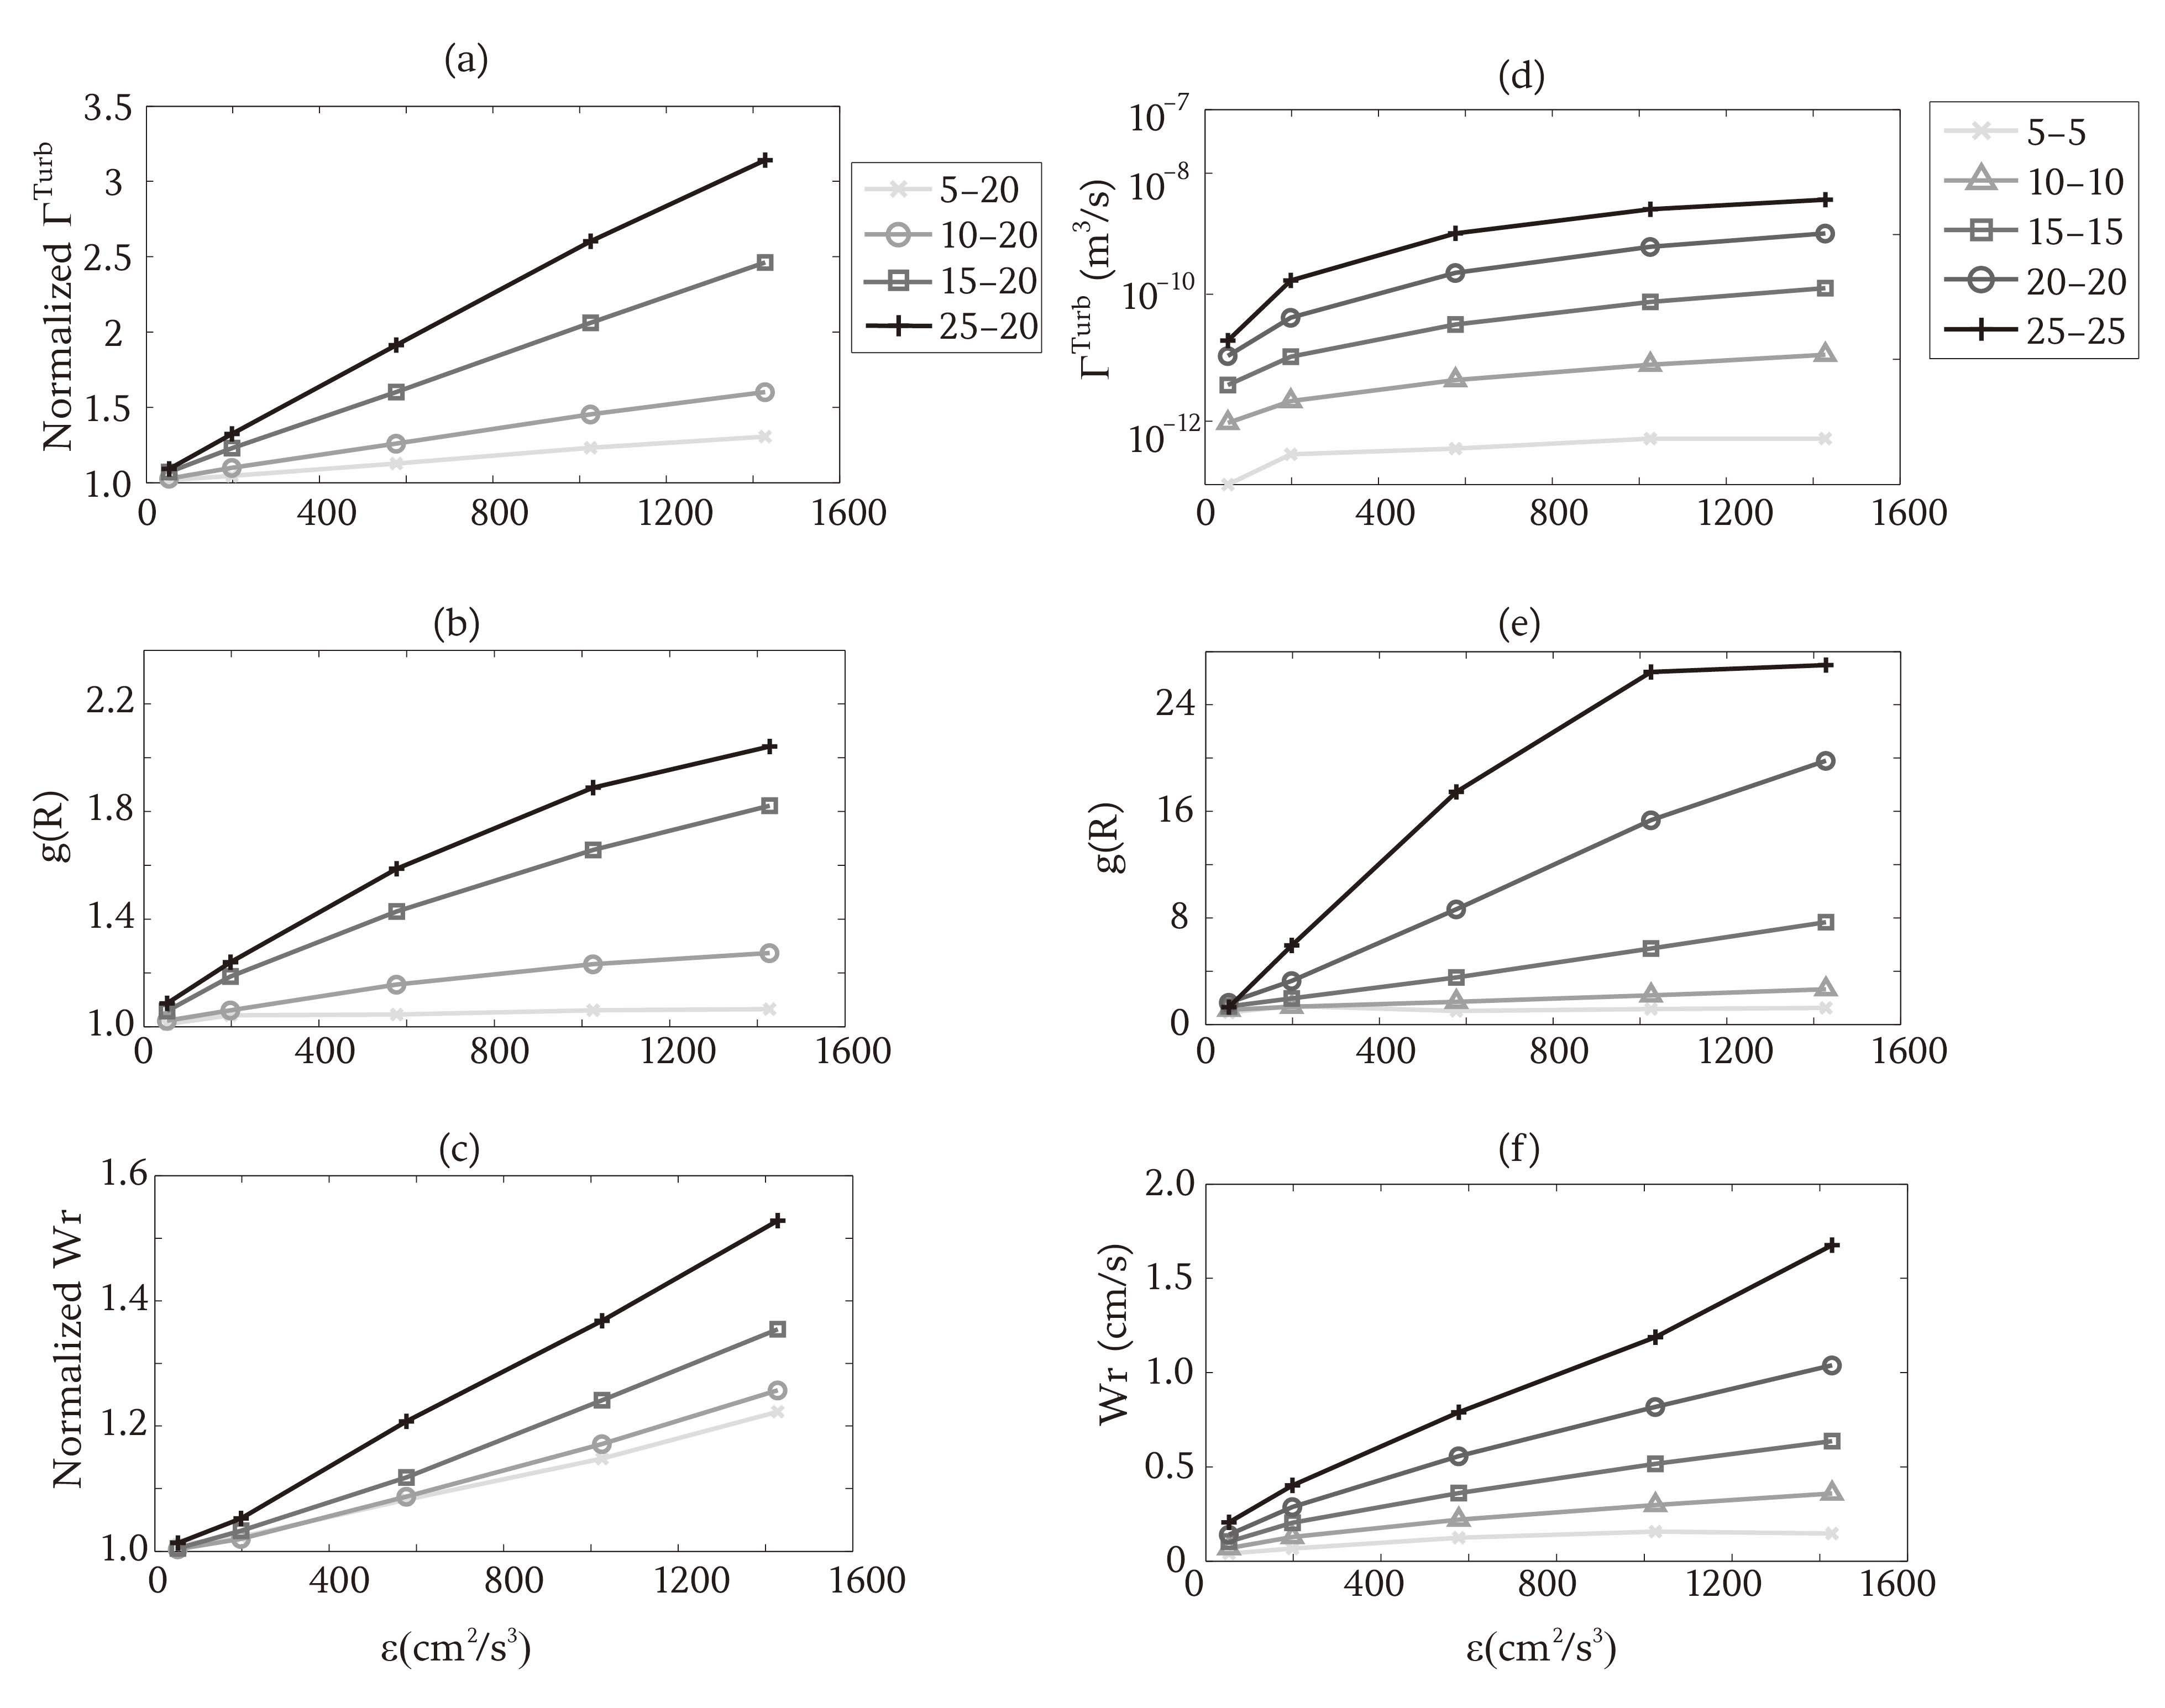
\includegraphics[width=0.8\textwidth]{Figures/Chap2/diss_cs_20_self.jpg} \caption{Collision statistics as a function of EDRs for cross-sized collisions involving 20 $\mu m$ droplets ((a)-(c)) and for same-sized collisions ((d)-(f)) } \label{fig:diss_cs_20_self}
\end{figure}

\section{Can we formulate a better collision parameterization?} \label{sec:ch2_parameterization}

We arrived at the conclusion that collision statistics for droplets of radius smaller than 25 $\mu m$ are insensitive to $R_\lambda$, implying the EDR and the pair sizes are the determining factors. As a consequence, we are of the opinion that parameterizations scaling with $R_\lambda$ are misleading. Here we introduce a modified parameterization scheme for turbulent collision kernels based on DNS data and at the same time attempt to match the forms of theoretical expressions from \citet{Saffman1956} and \citet{Wang1998b}.

\subsection{Turbulent collision kernel}

Given the dependence of the collision kernel on the EDR and droplet size, and the sensitivity test of $R_\lambda$ in section \ref{sec:ch2_result}, we applied curve fitting to our data to obtain a formula for the geometric collision kernel in the following form:
\begin{multline}
\Gamma^{Turb}=\Gamma^{Grav}+ 2\pi R^2 \Big[ \big(\frac{R}{\eta}\big)^{0.84}+(7 St_1 St_2)^{0.85}\Big]
 \times \sqrt{0.5\epsilon(|\tau_{p1}-\tau_{p2}|+0.3\sqrt{\tau_{p1}\tau_{p2}})}, \label{eqn:paragamma}
\end{multline}
where $St_i$ and $\tau_{pi}$ are the Stokes number and response time of the colliding droplets, respectively. The first term on the right-hand side is the gravitational collision kernel, which is $\pi R^2|V_{t2}-V_{t1}|$. The second term is the turbulence-enhanced component, which is the coupling of the clustering effect and the turbulent transport effect. The collision kernel, as demonstrated by DNS, is a function only of dissipation rate (as $\eta$ and $\tau_k$ can be derived from it) and droplet size; $R_\lambda$ and $u\prime$ are therefore excluded from the formula since they are both determined by the arbitrary size of the computational domain.

The predicted collision kernel calculated from the formula are shown in figure \ref{fig:parameterizations} (a) along with the results of our DNS. The parameterization reproduced the collision kernel correctly except for the case of same-sized collisions between 5 $\mu m$ droplets (the points in the lower left corner of the figure). Those collision events are not the major concern of our parameterization since they contribute very little to the overall droplet growth because of their low chance of colliding compared to other droplet pairs. Otherwise high accuracy in predicting the collision kernel is achieved by our parameterization. The relative error, which is calculated by normalizing the absolute difference between values from the parameterization and the DNS and taking the average, was used to measure the uncertainty of our parameterization scheme. The uncertainties came from a variety of sources. One was from poor sampling of same-sized collisions, especially for both the largest and smallest droplets, as mentioned in section \ref{sec:ch2_diss}; another source of uncertainty is simply the scatter resulting from finite-size ensembles of realizations.  The result shows that the uncertainty in predicting the cross-sized collision case was very small with a value of 6\%; however, for same-sized collisions, it was still significant (28\%). 


\subsection{Radial relative velocity}
\citet{Wang1998b} modified the analytical equation of RRV based on the studies of \citet{Saffman1956} and \citet{Hu1997} and proposed a more accurate formula:
\begin{multline}
\langle|\mathbf{W_r}|\rangle=\Big( \frac{2}{\pi} \Big)^{1/2}\bigg[ \frac{1}{15}R^2\frac{\epsilon}{\nu} + (\tau_{p2}-\tau_{p2})^2 \bigg\langle\bigg( \frac{Du}{Dt} \bigg)^2 \bigg\rangle \\
+ 2\tau_{p1}\tau_{p2} \bigg\langle \bigg( \frac{Du}{Dt} \bigg)^2 \bigg\rangle \frac{R^2}{\lambda_D^2} +\frac{\pi}{8}(\tau_{p2}-\tau_{p1})^2g^2\bigg]^{1/2}, \label{eqn:Wangpararrv}
\end{multline}
where $\frac{Du}{Dt}$ is the local fluid acceleration. $\lambda_D$ is the longitudinal Taylor microscale of fluid acceleration defined by $(\frac{1}{\lambda^2_D}) = -(1/2)\frac{\partial^2}{\partial x^2}f_D(0)$ and $f_D$ is the longitudinal correlation function of the velocity derivative. We fit curves to match our DNS data on the basis of their formula by keeping the local fluid shear term and gravity term (first and last term inside the square brackets) and modifying the fluid acceleration term and coupling term (second term and third term inside the square brackets) in a way that does not depend on $R_\lambda$ (i.e., without $\big\langle (\frac{Du}{Dt})^2\big\rangle$ and without the $\lambda_D$ term). The local fluid acceleration $\langle(\frac{Du}{Dt})^2\rangle$  and longitudinal Taylor microscale $\lambda_D$ are replaced with expressions involving EDR, which are the only way to use $\epsilon$ with $(\tau_{p1} - \tau_{p2})$ and $\tau_{p1}\tau_{p2}$ while keeping the same dimensions. We obtained the fit as follows:
\begin{multline}
\langle|\mathbf{W_r}|\rangle = \Bigg(\frac{2}{\pi}\Bigg)^{1/2} \Bigg\{\frac{1}{15}R^2\frac{\epsilon}{\nu} +\epsilon|\tau_{p2}-\tau_{p1}|\\
+ 0.001\epsilon\sqrt{\tau_{p1}\tau_{p2}}\bigg[ \bigg( \frac{R}{\eta}\bigg)^{0.1}-0.5 \bigg]
+\frac{\pi}{8}(\tau_{p2}-\tau_{p1})^2g^2 \Bigg\}^{(1/2)}, \label{eqn:pararrv}
\end{multline}
the first term inside the curly brackets measures the effect of local shear from turbulence, which is also the only remaining term when one considers only non-inertial particles. The second term denotes the different inertial response of the droplet pair to the local fluid acceleration. The third term is the overall response of the droplet pair due to local fluid acceleration, which is critical for same-sized collisions; the last term is the gravity term.  Figure \ref{fig:parameterizations} (b) demonstrates that the predicted RRV using the parameterization asymptotes to the observed value. For cross-sized collisions the gravity term has the largest contribution to RRV due to different terminal velocities; when colliding, droplet sizes get closer until they are equal, the gravitational effect diminishes and the local acceleration term (the third term) dominates. 

Our parameterization scheme for RRV performed with high accuracy for both the cross-sized collision case and the same-sized collision case. For cross-sized collisions, the average root-mean-square error (RMSE) of the normalized RRV (i.e. the RRV normalized by the value in the corresponding stagnant air case) was 0.03, which is much lower than \citet{Franklin2007}'s value of 0.28. The relative error was within 13\% which is slightly higher than that in \citet{Ayala2008b} (5\%). For same-sized collisions the relative error was 15\%, which improves upon \citet{Ayala2008b}'s parameterization where the relative error was 48\% for $\epsilon = 400 cm^2s^{-3}$. For a closer comparison, our relative error for $\epsilon = 500 cm^2s^{-3}$ was 14.73\%. Table \ref{tab:err} gives the relative errors of the collision statistics from our parameterization.

\subsection{Radial distribution function}
To quantify the clustering effects in a turbulent cloud system we also parameterized the RDF. We attempted to simply apply the analytical formula of the collision kernel \eqref{eqn:sph}. Therefore, $g(R)= \frac{\Gamma^{Turb}}{(2\pi R^2 \langle |\mathbf{W_r}| \rangle )}$, where $\Gamma^{Turb}$ and $\langle |\mathbf{W_r}| \rangle$ were obtained from the parameterizations derived in the previous section. However, the quotient of $\Gamma^{Turb}$ and $\langle |\mathbf{W_r}| \rangle$ led to amplified error. Even though the average relative error was small (0.19), the parameterized RDF had a group of values below unity, which is unreasonable. Therefore this simple method was proved incapable to evaluate the clustering effects in a quantitative sense, but it can still help to make a qualitative assessment, which is easier to calculate than the following method we will introduce. 

\citet{Ayala2008b} developed an empirical formula for g(R) that includes both same-sized collisions and cross-sized collisions (see equation \eqref{eqn:parardf}  below). However their parameterization is a function of $R_\lambda$. This caused a spread of g(R) under the same EDR but over a broad range of $R_\lambda$. The average error using this method was 0.18 and was largely caused by the spread. To remove the $R_\lambda$ effect, we modified their formula by replacing the terms that contained $R_\lambda$ with constants in order to fit our data. The overall structure was the same but the calculation of terms of $r_c$ and $C_1$ was simplified. $r_c$ and $C_1$ depended on the $R_\lambda$ in their original paper. Here we used constants to replace those terms and their formulas are given below: 
\begin{equation}
g(R)=(\frac{\eta^2+r_c^2}{R^2+r_c^2})^{C_1/2}, 
 \label{eqn:parardf}
\end{equation}

\begin{equation}
C_1=\frac{y(St)}{[|{\bf g}|/(v_k/\tau_k)]^{0.36}},
\end{equation}

\begin{equation}
(\frac{r_c}{\eta})^2=|St_1-St_2|\times F,
\end{equation}

\begin{equation}
F=20.115 \times \Big[{\frac{15 + \frac{\pi}{8}\big(\frac{|\bf{g}|}{v_k/\tau_k}\big)^2}{200}}\Big]^{1/2}.
\end{equation}

Here $y(St)$ is a fitted polynomial function of $St$ fitted based on their DNS experiments; $v_k = (\nu\epsilon)^{1/4}$ is the Kolmogorov velocity. 

The parameterized $g(R)$ matched well the simulations with an average relative error of 0.12 (see figure \ref{fig:parameterizations}(c)). The red dots from the DNS simulations with values below 1 originated in 5-5 $\mu m$ collisions and were caused by poor sampling as these droplets have little possibility to collide with each other and their pair statistics were based on less than 3000 collisions. 

\begin{table}[ht]
\caption{Relative errors for the parameterization of the collision statistics, for same-sized collisions, cross-sized collisions, and the average for all collisions\strut} \label{tab:err}
\begin{center}
\def\arraystretch{1.5}
\begin{tabular}{cccc}
\hline\hline
 & Same-sized collision & Cross-sized collision & Average \\
\hline
$\Gamma^{Turb}$ & 0.28 & 0.06 & 0.14\\
\hline
$\mathbf{W_r} $ & 0.15 & 0.13 & 0.14 \\
\hline
g(R) & 0.21 & 0.07 & 0.12 \\
\hline
\end{tabular}
\end{center}
\end{table}
\begin{figure}[ht]
\centering
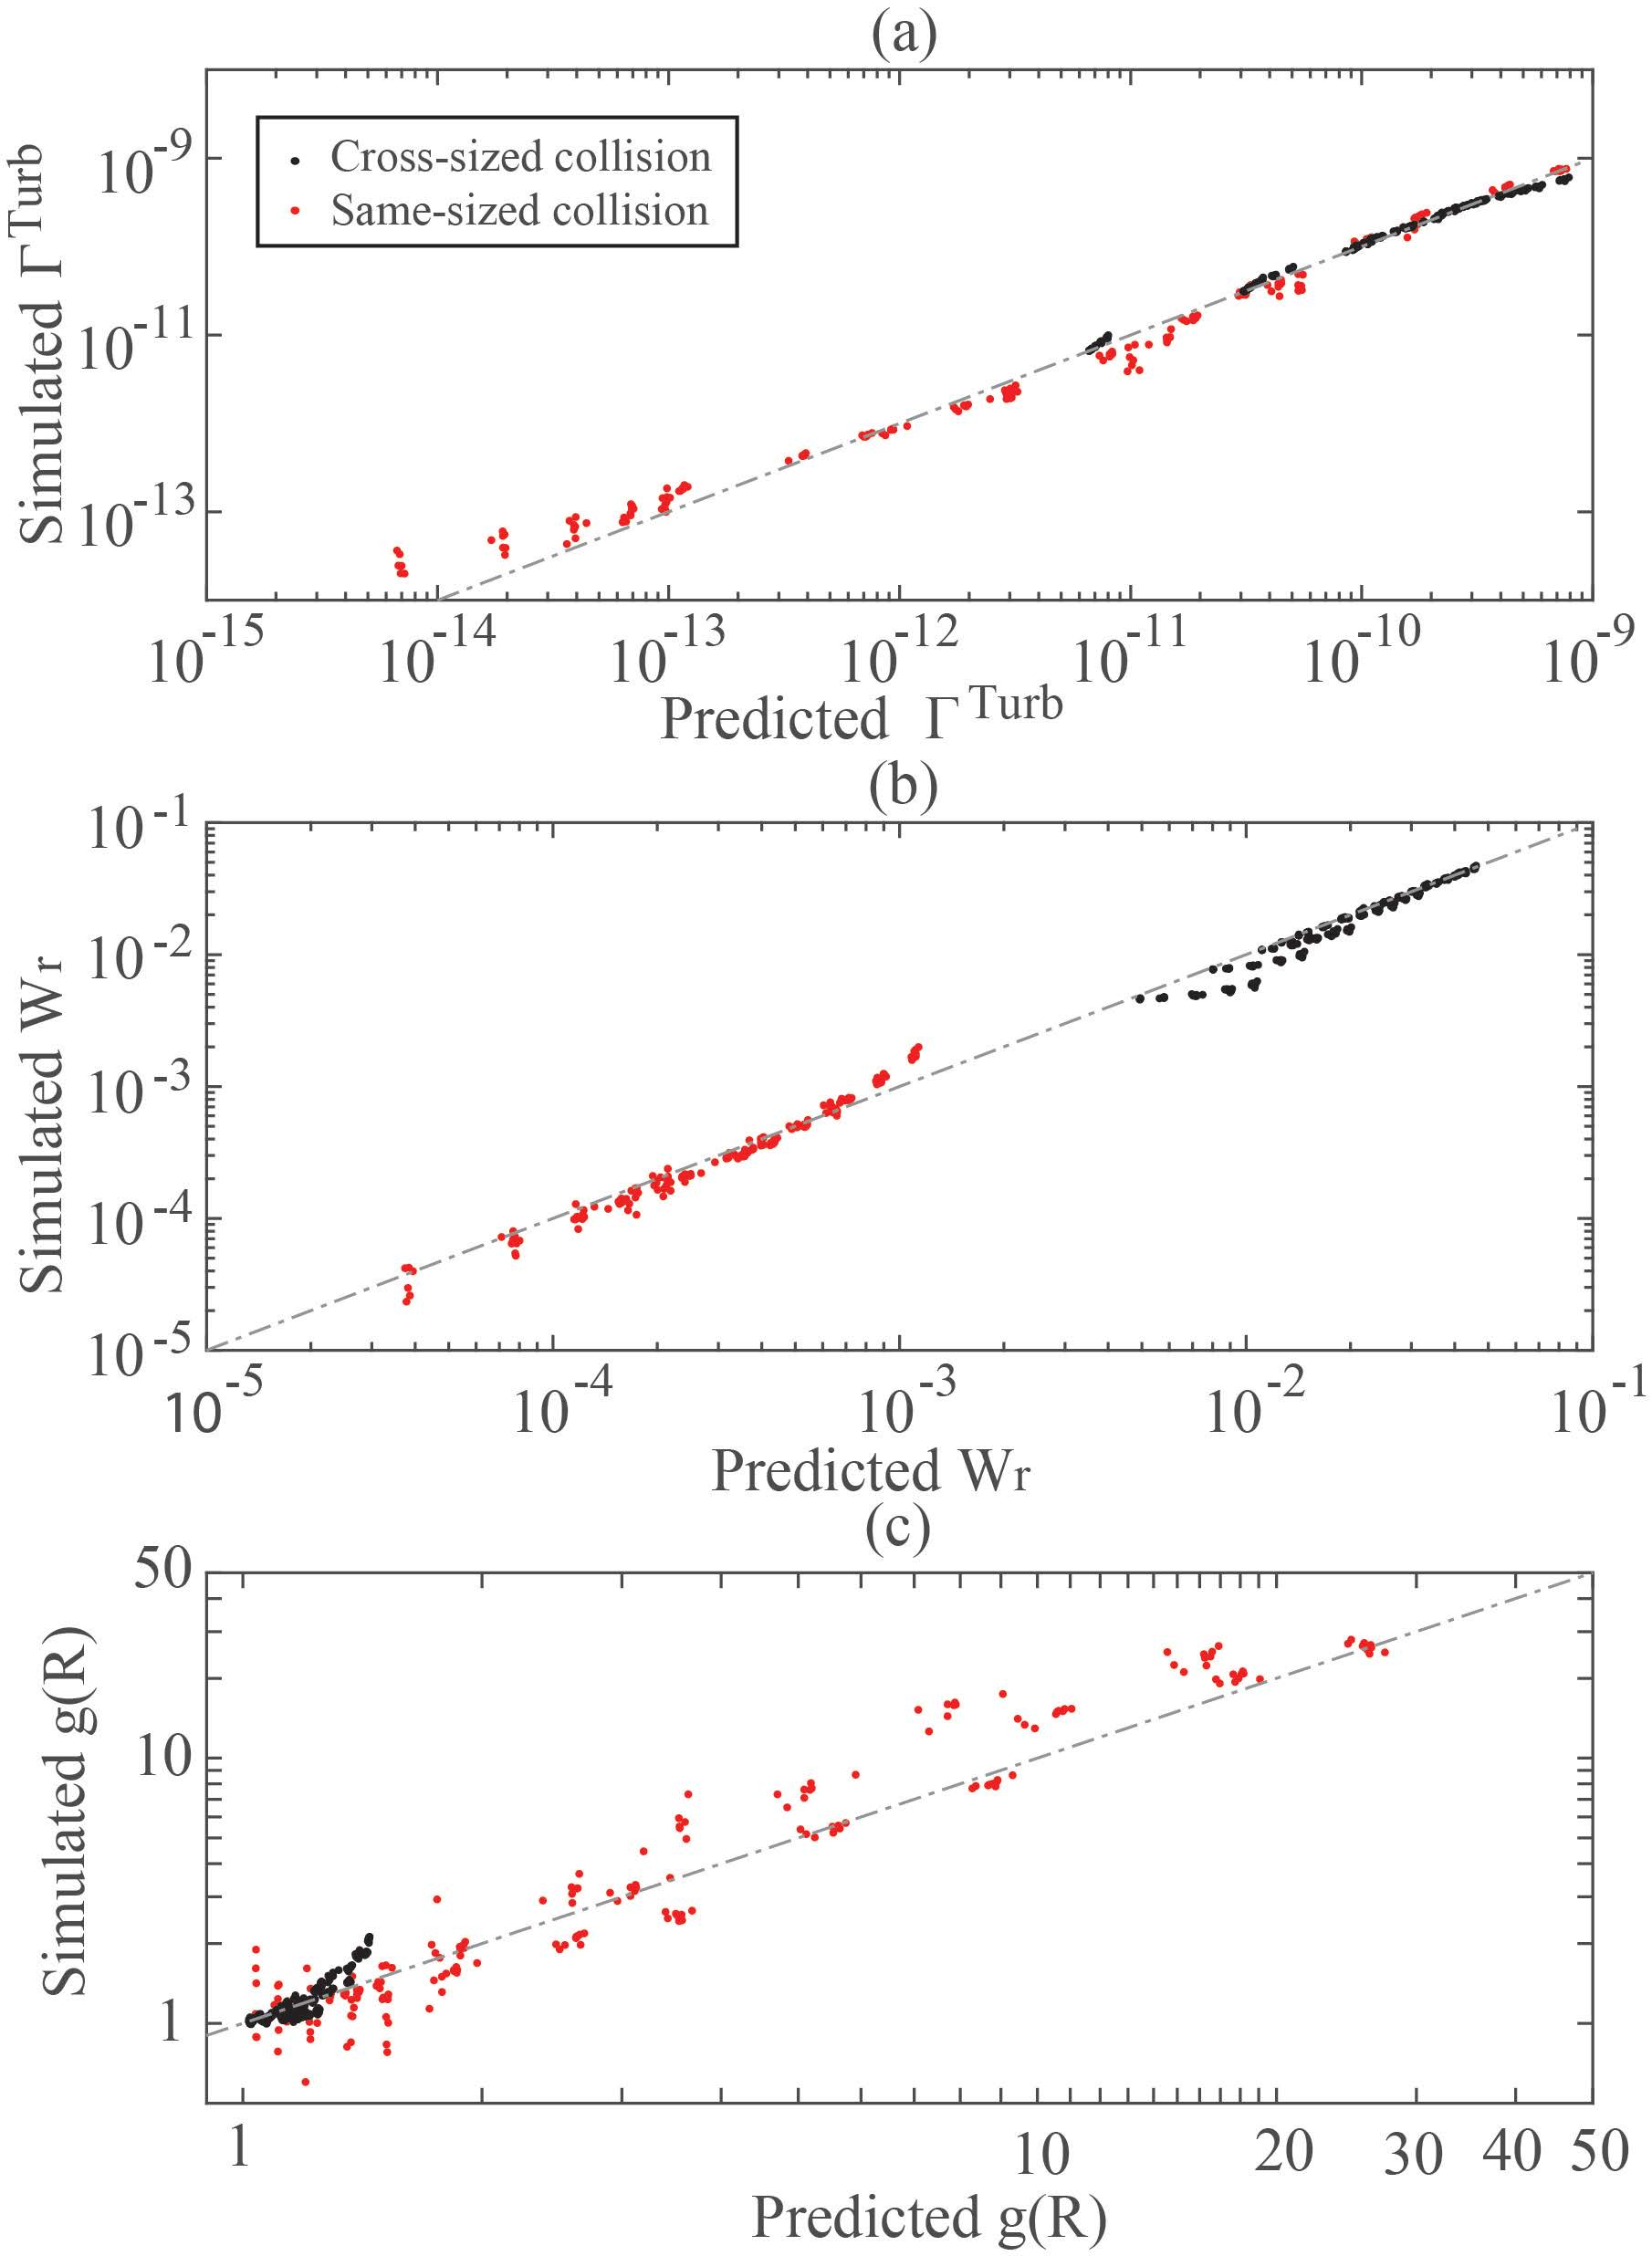
\includegraphics[width=0.6\textwidth]{Figures/Chap2/parameterizations.jpg}\\
\caption{(a) collision kernel ($m^3 s^{-1}$), (b)  RRV ($cm s^{-1}$), and (c) RDF from the DNS against their corresponding parameterized value for cross-sized collisions (black dots) and same-sized collisions (red dots). Different dots represent statistics of different droplet pairs with different turbulent conditions.} \label{fig:parameterizations}
\end{figure}

\subsection{Comparisons with DNS data and other models}
In this section, a brief comparison of our prediction model with other studies \citep{Franklin2007, Saffman1956, Wang1998b, Zhou2001, Ayala2008b} is given. We compared the turbulence enhancement of the collision kernel between 10 $\mu m$ - 20 $\mu m$ droplets and that of 10 $\mu m$ - 15 $\mu m$ with different eddy dissipation rates. 

The DNS results of \citet{Ayala2008a} were obtained from their largest $R_\lambda$(=72.4) case where we assumed sufficient scale separation has been achieved such that $R_\lambda$ does not affect the collision statistics. Figure \ref{fig:colker} shows that the difference between our DNS results and their results was insignificant. The collision kernel from \citet{Franklin2005} grew faster than the other models by a factor of 1.65 due to the difference in calculating flow parameters, discussed in section \ref{sec:ch2_flowpara}, suggesting that their parameterization yields significant overestimation of the collision kernel (see blue dashed line in figure \ref{fig:colker}). The studies from \citet{Wang1998b} and \citet{ Saffman1956} did not consider the clustering effect and consequently underestimate the values (see dashed curves with light green and gray, respectively). The RDF by \citet{Zhou2001} was parameterized based on a non-sedimenting assumption. Thus one would expect some overestimation \citep{Xue2008} because droplets would stay in clouds longer without sedimentation. However, even after including the clustering effect given by \citet{Zhou2001}, the curve of \citet{Wang1998b} was still lower than the DNS data, even though it displayed a similar slope (see dark green curve in figure \ref{fig:colker}). 
\citet{Pinsky2006collision} developed a model in which the turbulence was represented using a statistical formulation. Therefore, large Reynolds numbers were achieved in their study. Since their model did not include clustering effects, underestimation was expected in the collision kernel. We compared their curve of collision kernel of 10-15 $\mu m$ pair statistics with the DNS data (not shown in figure); larger underestimation was found at low intensities (stratiform clouds and cumulus clouds as categorized by their paper in the bottom of figure 7). By contrast, our parameterization scheme performed well at low EDRs and deviated slightly from the DNS data as the dissipation rate became higher (see figure \ref{fig:colker}), implying a good performance in predicting stratiform to cumulus clouds (with an EDR less than $\approx 600 cm^2s^{-3}$).  Overall, most of the parameterization schemes underestimated the turbulent enhancement except for the curve of \citet{Ayala2008b} (purple dashed curve). Although our parameterization showed some uncertainties, its results still show a good fit to the DNS.

\begin{figure}[ht]
\centering
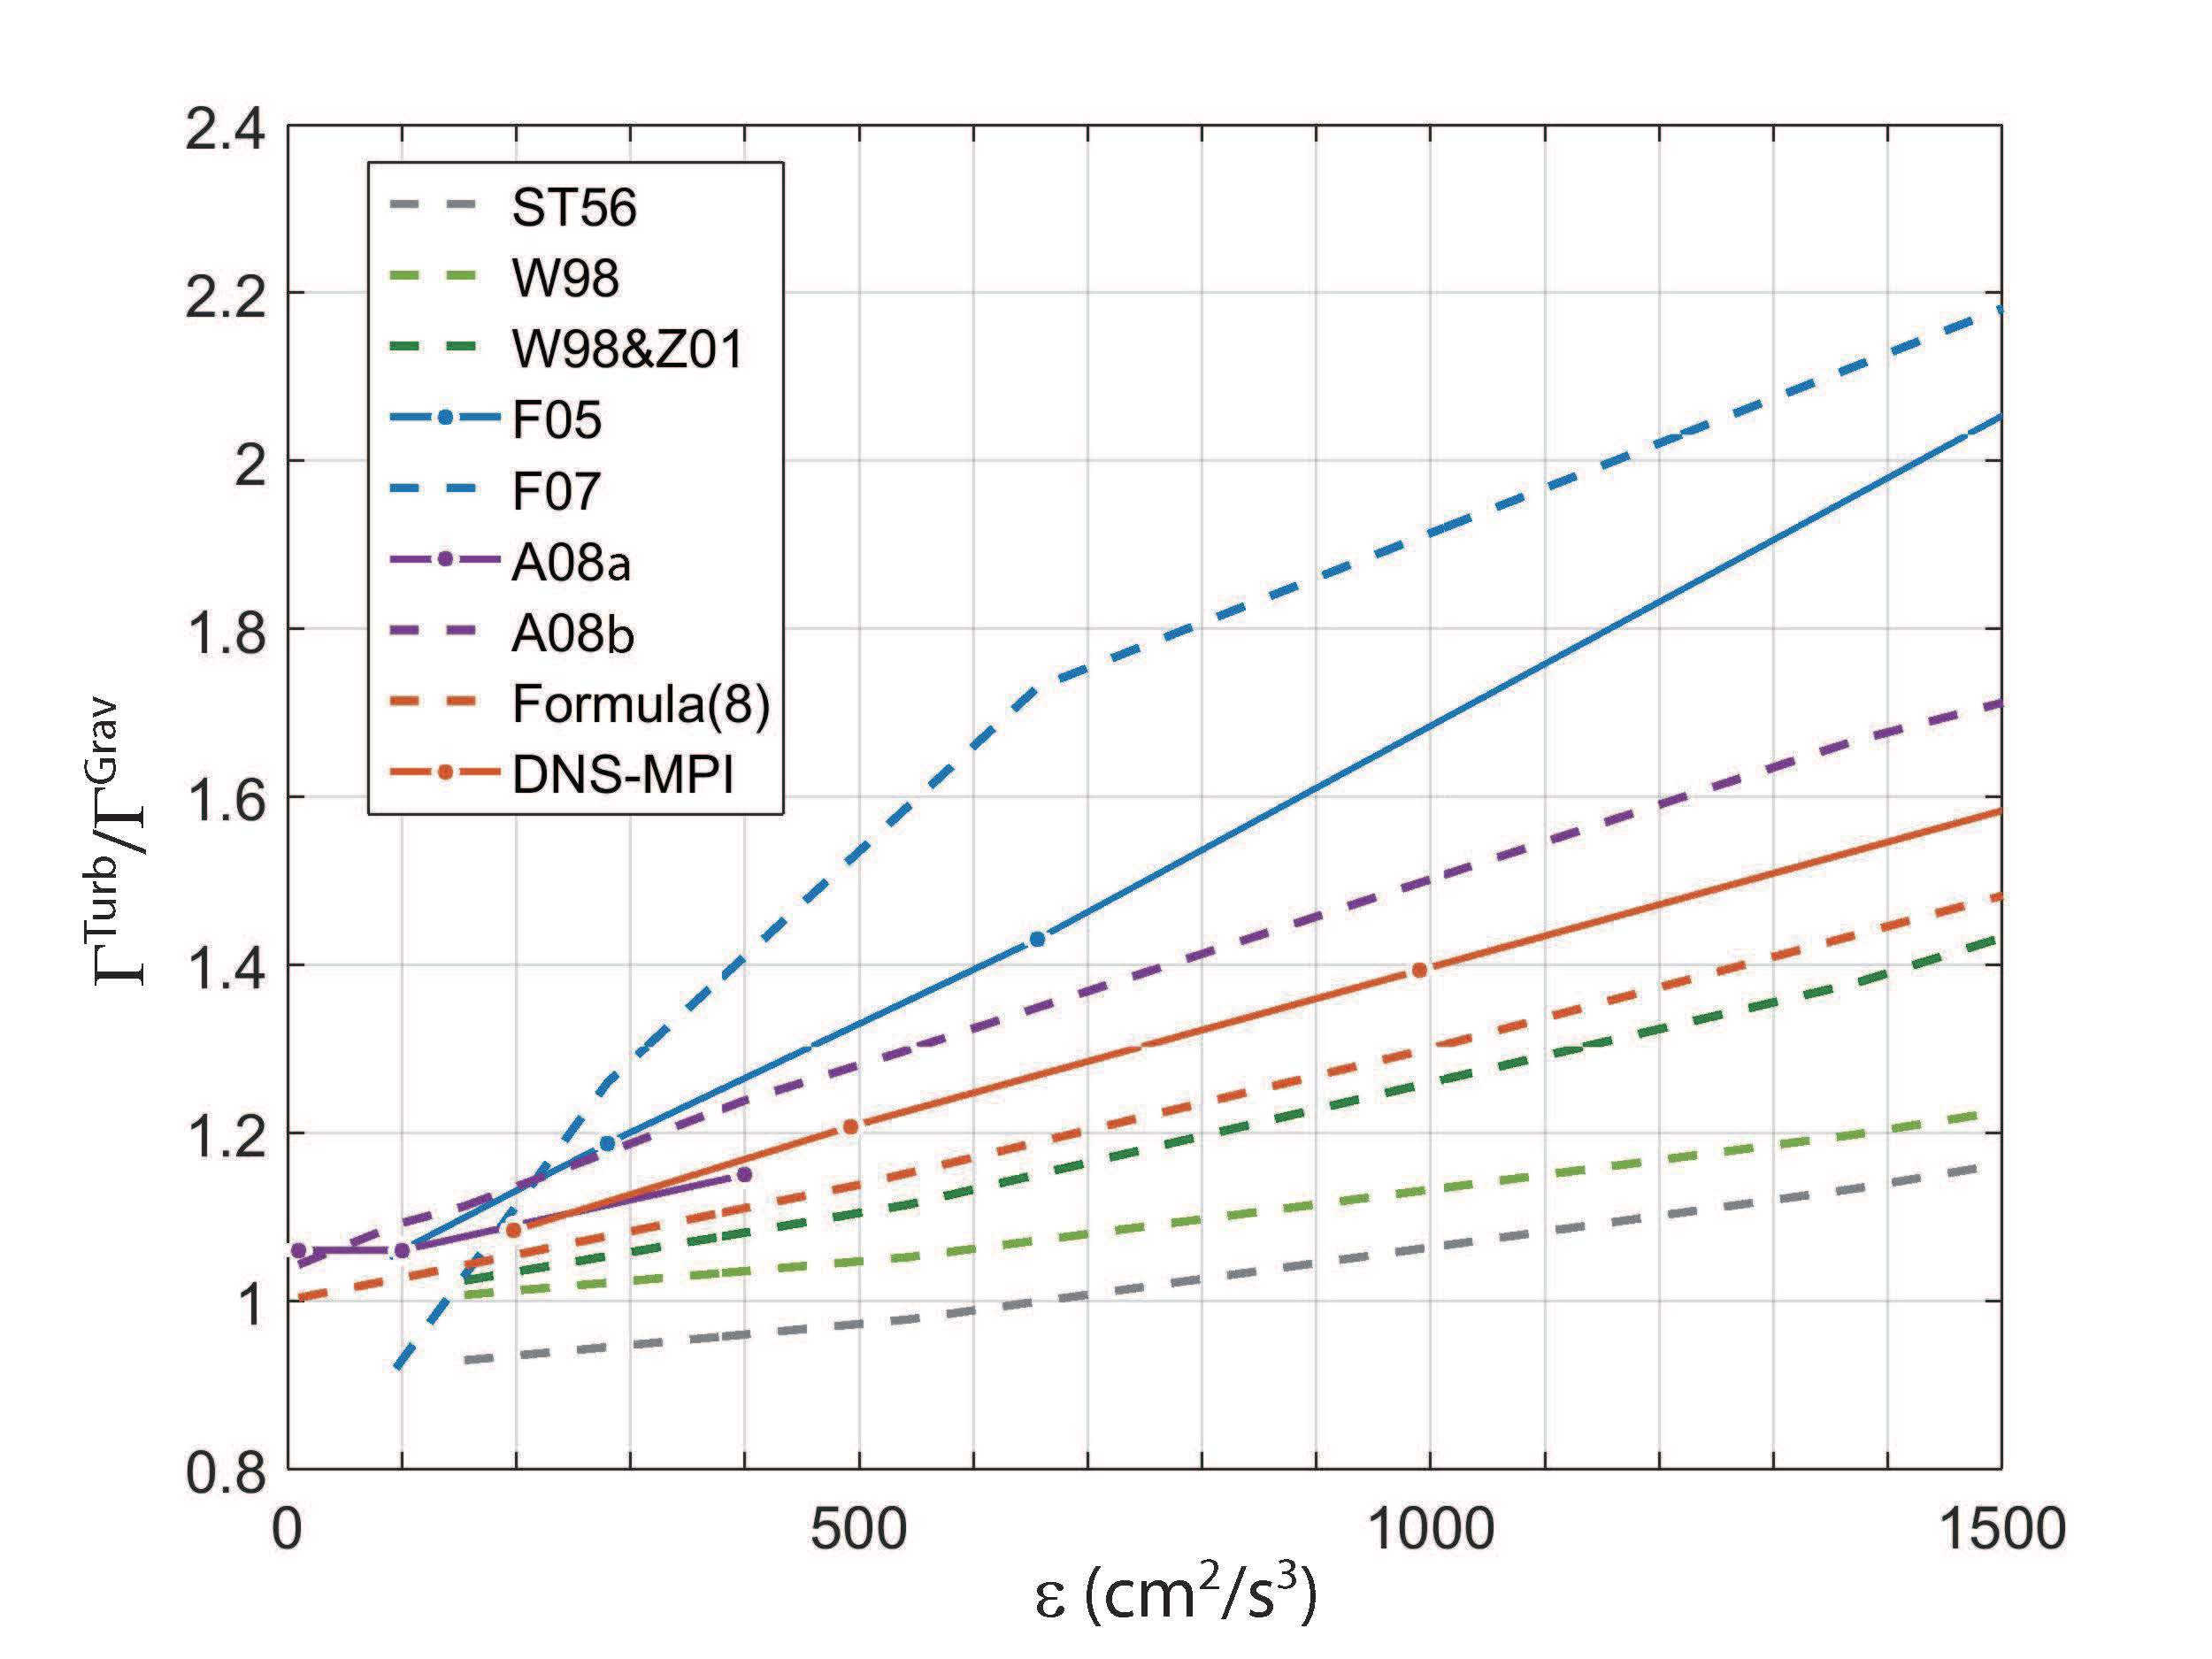
\includegraphics[width=0.7\textwidth]{Figures/Chap2/compares.jpg}  \\
\caption{Ratio of turbulent collision kernel and gravitational collision kernel for droplet pairs of 10-20 $\mu m$ as a function of EDRs from different studies \citep{Saffman1956, Wang1998b, Zhou2001, Ayala2008a, Ayala2008b, Franklin2005, Franklin2007}. Solid lines represent results obtained from simulations of various models; dashed lines represent parameterized values; different colors marks different studies. The lines in brown are from this study. }\label{fig:colker}
\end{figure}

\section{Summary and discussion} \label{sec:ch2_conclusion}

In this study we examined the major question of warm rain initiation: what role does turbulence play in droplet collisional growth? And can we obtain a more accurate parameterization? With the help of DNS, we quantified the turbulence effect in droplet growth by collision-coalescence based on 39 successful runs (including five different eddy dissipation rates and nine different Reynolds numbers or computational box sizes) with 15 different combinations of droplet pairs in the appropriate range for real clouds to initiate collision-coalescence processes. We studied three collision statistics (RRV, RDF, and turbulent collision kernel) between droplets of radius less than 25 $\mu m$ using a model configuration different from \citet{Franklin2005}, which allowed us to successfully separate the effect of $R_\lambda$ from $\epsilon$, or EDR. We found that all collision statistics were insensitive to $R_\lambda$ over the range of box sizes we can afford to simulate and as long as the model resolved all the smallest scales of turbulence (i.e., the Kolmogorov length scale). This implies that the droplet motions and their collision statistics are mainly affected by the smallest fluid scales, and that the large-scale motion has negligible influence. Moreover, the collision statistics were found to be strongly correlated with the EDR and the size of droplets. Therefore, we developed a parameterization, which is independent of $R_\lambda$ and $u\prime$ and instead is dependent on turbulence intensity ($\epsilon$ or EDR), the fluid properties ($\rho_a, \nu$, etc.), and the droplet sizes. 

We proposed a form of the collision kernel that includes both same-sized collisions and cross-sized collisions and thus is able to describe the continous growth of droplets by collisions. The parameterized collision kernel was demonstrated to be highly consistent with DNS results. The formula predicted the turbulent collision kernel with an error of 15\% on average, better than other proposed formulas. We also parameterized the RRV and RDF, which offers future model developers a measure of the turbulence effect on the relative motion and spatial distribution of droplets. Their average relative errors were 14\% and 16\%, respectively. Again, an improvement over previous studies. 

It is recognized that the droplet growth rate is also determined by other factors such as the collision efficiency and condensational growth. To accurately parameterize the effect of turbulence on cloud droplet growth, the next step is to include these mechanisms. 

\acknowledgments
Computations were mainly made on the supercomputer Mammouth II parall\`{e}le from Universit\'{e} de Sherbrooke, managed by Calcul Qu\'{e}bec and Compute Canada. The operation of this supercomputer is funded by the Canada Foundation for Innovation (CFI), NanoQu\'{e}bec, RMGA and the Fonds de recherche du Qu\'{e}bec - Nature et technologies (FRQ-NT). Part of the simulations were run on the supercomputer SGI Altix 4700 from Universit\'{e} de Montr\'{e}al. This work was supported by the Natural Sciences and Engineering Research Council of Canada (NSERC). 

\cleardoublepage 


%========== Chapter 3 
\typeout{}
\resetdatestamp

\chapter{Turbulence impact on collision efficiency and broadening of droplet size distribution}\label{sec:ch3}

%\epigraph{Truth, like gold, is to be obtained not by its growth, but by washing away from it all that is not gold.}{\emph{Leo Tolstoy} (1828 -- 1910)}
In Chapter \ref{sec:ch2} we have studied the turbulence impacts on the droplet geometric collisions by investigating the turbulent enhancement of collisions through the droplet clustering effect and the relative velocity effect. In this chapter we will study the turbulent enhancement of the hydrodynamic collisions in order to answer the following research question: How does turbulence impact the droplet hydrodynamic interaction and thus modify the collision efficiency? The droplet disturbance flow fields are resolved by the model, and thus the hydrodynamic interactions between neighbouring droplets are considered. The first part of this chapter examines and quantifies the turbulence effect on the droplet collision efficiency and the hydrodynamic collision rate. In the second part of this chapter we scrutinize the evolution of the droplet size distribution in various turbulent environments by allowing droplets to grow by collision-coalescence. 

This chapter consists of a paper published in the Journal of the Atmospheric Sciences: Sisi Chen, M.K. Yau, and Peter Bartello: Turbulence effects of collision efficiency and broadening of droplet size distribution in cumulus clouds, \url{https://journals.ametsoc.org/doi/abs/10.1175/JAS-D-17-0123.1}
\newpage
\newpage

\section*{\centering Turbulence effects of collision efficiency and broadening of droplet size distribution in cumulus clouds}
\begin{center}
\author{ Sisi Chen, M. K. Yau, Peter Bartello \\  \textit{Department of Atmospheric and Oceanic Sciences, McGill University, Montr\'{e}al, Qu\'{e}bec, Canada}\\} 
\end{center}

\section*{\centering Abstract}
This paper aims at investigating and quantifying the turbulence effect on droplet collision efficiency and exploring the broadening mechanism of droplet size distribution (DSD) in cumulus clouds. The sophisticated model employed in this study individually traces droplet motions affected by gravity, droplet disturbance flows, and turbulence in a Lagrangian frame. Direct numerical simulation (DNS) techniques are implemented to resolve the small-scale turbulence. Collision statistics for cloud droplets of radius between 5-25 $\mu$m at five different turbulence dissipation rates ($20-500 $ $cm^2s^{-3}$) are computed and compared with pure-gravity cases. The results show that the turbulence enhancement of collision efficiency highly depends on the r-ratio but is less sensitive to the size of the collector droplet investigated in this study. Particularly, the enhancement is strongest among comparable-sized collisions, indicating that turbulence can significantly broaden the narrow DSD resulting from condensational growth. Finally, DNS experiments of droplet growth by collision-coalescence in turbulence are performed for the first time in the literature to further illustrate this hypothesis and to monitor the appearance of drizzle in the early rain formation stage. By comparing the resulting DSDs at different turbulence intensities, it is found that broadening is most pronounced when turbulence is strongest and similar-sized collisions account for 21-24\% of total collisions in turbulent cases compared to only 9\% in the gravitational case.

\section{Introduction}\label{sec:ch3_intro}

Warm clouds, such as trade wind cumuli, are one of the most common types of clouds on Earth. Cloud radar observations show that shallow convective systems can initiate rain very rapidly and sometimes can produce very heavy precipitation \citep{Stevens2016}. The understanding of this fast and efficient rain initiation represents a longstanding challenge in the cloud physics community as it involves complicated microphysical and macro-physical processes. 

In the development of cloud and rain, a major growth process is the collision between droplets. For collisions to occur, a broad droplet spectrum is favored to guarantee a significant difference in droplet terminal velocities so that droplets can efficiently encounter one another. In addition, some larger droplets must be present because the collision efficiency between much smaller droplets becomes negligible. To set the stage for collision, cloud droplets first grow by condensation. However, as discussed in classic condensational growth theory, the droplet growth rate in terms of radius varies inversely with radius in an adiabatic environment. As such, broad spectra or large droplets, which are both observed in in-situ measurements \citep[e.g.,][]{Khain2013}, are unlikely to be achieved in a reasonable time scale. For example, \citet{Jonas1996} showed that a droplet in still air takes 20 minutes to grow from 10 to 20 $\mu$m by condensation under 0.2\% supersaturation and a further hour to grow by collision-coalescence to reach drizzle size (see his Fig. 4).This time scale is much longer than observed. 

In the last half century, turbulence in clouds has been proposed to explain the fast warm-rain initiation due to the enhancement of the collision rate. Nevertheless, the effects of turbulence on droplet collisions, especially on the collision efficiency, are not well-quantified. As a result, the coupling between turbulence and microphysics is absent in most cloud resolving models. Despite the fact that clouds are turbulent, the inclusion of the effects of turbulence on the collision kernel and the collision efficiency remains problematic \citep{Grabowski2013}. 

At present, no formulas or theories have been established to describe the turbulent collision efficiency due to the complexity of the droplet behavior under the effect of the disturbance flow and turbulence flow, we mainly rely on numerical studies to offer tabulated values to provide the relationship between the turbulent intensity and the collision efficiency \citep[for example, ][]{Pinsky2008, Wang2008}. Statistical modeling of the turbulent collision efficiency in the past has yielded a wide spectrum of results. The problem arises mainly from the various inaccurate assumptions and treatments of turbulent flow fields and droplet motions due to limited computational power \citep{Grabowski2013}. For example, in most simulations the relative motion of droplets is assumed equal to the difference of their gravitational terminal velocity when the separation distance is more than a few droplet diameters apart. This assumption restricts the effects of turbulence to be within the viscous subrange \citep{Pinsky1997}. On the other hand, no unanimous conclusions have been reached by those studies which used different statistical turbulence approaches. For example, \citet{Almeida1979} found that the collision efficiency was enhanced in turbulence by an order of magnitude. However, his model suffered from a major drawback in that small-scale turbulence was represented by an inertial subrange scaling, while droplet interaction is believed to happen at the viscous scale \citep{Pinsky1997}. The \citet{Pinsky2004} stochastic model showed a strong effect of turbulence on collision efficiency for droplets less than 10 $\mu$m in radius while \citet{Pinsky2007} demonstrated that turbulence enhancement of collision efficiency was strongest among droplets of similar sizes and small droplets a few microns in radius. However, their turbulence was generated from a large set of random Fourier modes, which is unable to reproduce the intermittent phase coherence of a turbulent flow. In contrast, \citet{Koziol1996} showed no significant enhancement of collision efficiency by turbulence. However, their collision efficiency also included the turbulence enhancement on the geometric collision kernel and is thus not directly comparable to other studies. 

As computational power continues to expand, we can explicitly resolve the dissipation range of turbulent flows in a Direct Numerical Simulation (DNS) framework, and track the Lagrangian history of each droplet. Earlier DNS studies by \citet{Franklin2005,Franklin2007}, \citet{Ayala2008a}, and \citet{Chen2016} focused on quantifying the turbulence effect on the geometric collision kernel, $\Gamma^{GEO}$, (i.e., collision kernel without considering hydrodynamic droplet interactions) and they all arrived at the conclusion that turbulence strengthens droplet clustering and enhances the relative motion between two colliding droplets. To quantify the turbulent collection kernel $\Gamma^{CK}$, the collection efficiency $E(r_1,r_2)$ should be resolved as $\Gamma^{CK}=\Gamma^{GEO}\times E(r_1,r_2)$, where $r_1$ and $r_2$ are the droplet radii involved in the collision. $E(r_1,r_2)$ is the product of the collision efficiency and the coalescence efficiency ($E_{coal}$). The latter has a value close to unity for cloud droplets according to previous laboratory results \citep[Fig. 14-10 (a) of][]{Pruppacher1997} and most studies assume that $E_{coal}=1$ for simplicity \citep{Rogers1989}. Consequently, the collection efficiency can be approximated by the collision efficiency and the collection kernel approximated by the collision kernel.

To obtain an accurate collision efficiency, \citet{Wang2005a,Wang2005b} proposed an accurate superposition method to explicitly resolve the disturbance flow of two or more interacting droplets based on the assumption of Stokes flow. \citet{Ayala2007} developed a hybrid-DNS approach to study the turbulence effect on droplet hydrodynamic interaction based on the superposition method. With the same model, \citet{Wang2008} found that the collision efficiency for similar-sized droplet collisions can be increased by a factor of 4 at a dissipation rate of 400 $cm^2s^{-3}$, compared to the purely gravitational case (Fig. 13 in their paper). This enhancement is more than twice the geometric collision kernel enhancement, which implies that including the turbulent enhancement on collision efficiency can significantly affect the autoconversion rate, defined as the rate at which cloud droplets grow to form drizzle drops. Recent studies have provided improved or new numerical approaches to increase the accuracy of computing the collision efficiency but they are either not available to study the turbulent collision efficiency \citep{Rosa2011}, or deficient in quantitative evaluation \citep[e.g.,][]{Onishi2013, Ayala2014}. \citet{Wang2008} so far offers the most accurate and complete turbulent collision efficiencies but still suffers from several shortcomings. First, since their studies only involved two eddy dissipation rates (i.e., 100 $cm^2s^{-3}$ and 400 $cm^2s^{-3}$), simple extrapolation or interpolation from two data points results in large uncertainties. Second, the study did not consider collector droplets less than 20 $\mu$m that are still important for warm rain initiation. Besides, the liquid water content (LWC) used was much higher than typical adiabatic values, which might overestimate the cumulative effect of many-body aerodynamic interactions due to the resulting small separation distances between droplets and thus affect the collision efficiency. 

To address these shortcomings, this study gives a comprehensive investigation of the turbulence effect on collision efficiency for cloud droplets before the effective gravitational-collisional growth stage ($r < 30 $ $\mu$m) with a wide range of eddy dissipation rates ($20$ $cm^2s^{-3}<\epsilon<500$ $cm^2s^{-3}$) covering most observed values from cumulus clouds. LWC is set to be within the range of typical adiabatic values. In addition, this study provides the first attempt to directly simulate the droplet growth by collision-coalescence with DNS to allow for a quantitative evaluation of the entire droplet size distribution (DSD) broadening in different turbulent environments. We expect that the cloud physics community seeking data to support the study of the parameterization of collision efficiency and autoconversion rate, as well as the mechanisms of DSD broadening in fast warm rain initiation, will benefit from this work.

The paper is organized as follows: section \ref{sec:ch3_model} describes the DNS model and the methodology used. Section \ref{sec:ch3_result} presents the turbulent collision efficiency of different droplet pairs, which shows that turbulence significantly enhances the collision efficiency between similar-sized droplets. In section \ref{sec:ch3_reDSD}, results from simulations of DSD evolution at different turbulence dissipation rates are illustrated and discussed to further explore the turbulence broadening mechanism. Summary and conclusions are given in section \ref{sec:ch3_conclusion}.

\section{Model description} \label{sec:ch3_model}
A detailed description of the model can be found in Chapter \ref{sec:ch2}. The major difference is that in this paper, we include the flow fields induced by the neighboring droplets, so called the droplet disturbance flow. Besides, to observe DSD evolution, droplets are allowed to merge and grow by collision. For simplicity, we briefly explain the model framework with emphasis given to the improvements made to resolve the droplet motion. 

\subsection{Turbulent flow field}\label{sec:ch3_turb}

The turbulence in our simulations is statistically homogeneous and isotropic, which characterizes the environment of adiabatic cores in cumulus clouds \citep{Vaillancourt2000}. It is generated by solving the vorticity version of the incompressible Navier-Stokes equations (equation (\ref{eqn:NS1}) and equation (\ref{eqn:NS2})). The pseudo-spectral technique \citep{Orszag1969} is used to solve the equation, and triply-periodic boundary conditions are applied. Kinetic energy is constantly injected into a low-wavenumber band to maintain statistical stationarity. In Chapter \ref{sec:ch2}, we suggested a simple modification to the forcing scheme of \citet{Sullivan1994}, which greatly improves the efficiency in obtaining the desired mean dissipation rates. In this new forcing, an equal amount of energy is injected into the forcing band at each time step, instead of fixing the total kinetic energy in the forcing band. At statistical stationarity, the amount of energy injection, $KE_{in}$, at each time step, $\Delta t$, can be easily determined by the desired eddy dissipation rate, $\epsilon_0$, i.e., $KE_{in}=\epsilon_0 \Delta t$. 

The domain size for each simulation is on the order of $10cm$, with 64 grid points in each direction, which has been proved sufficient to obtain reliable collision statistics (see Fig. \ref{fig:Re_ck}). Physically, the model is robust as long as it resolves the collision-related scales, which are comparable to the mean droplet separation distance. In cumulus clouds, this distance is close to the Kolmogorov scale, $\eta$. Since $\eta$ describes the smallest energy-containing eddies below which viscosity dominates, the maximum resolvable wavenumber, $k_{max}$, which determines the grid size, $\Delta x$, is constrained to yield $k_{max}\eta > 1$. We fixed $k_{max} \eta=1.3$, to be on the safe side. Given $\eta = (\nu^3/\epsilon)^{1/4}$, where $\nu=1.6 \times 10^{-5}$ $m^2s^{-1}$ is the viscosity, it follows that a one-to-one negative correspondence can be established between $\Delta x$ and $\epsilon$ (see Section \ref{sec:ch2_separate}). As turbulence gets weaker, the size of the grid boxes keeps expanding, consequently including more droplets and requiring more computation. According to observations, a typical range of dissipation rates for shallow cumulus clouds is from 10-100 $cm^2s^{-3}$ \citep{siebert2013}. To ensure simulations close to observations and computationally feasible, the dissipation rate ranges from $20-500 $ $cm^2s^{-3}$  in this study. 

\subsection{Droplet motion and disturbance flow field} \label{sec:ch3_drop}

We mainly consider droplets of radii from 5-25 $\mu m$ because they are crucial to forming larger droplets to initiate effective gravitational collisional growth. Droplets are randomly placed throughout the domain after the turbulence reaches statistical stationarity (i.e., energy spectra stabilize and -5/3 law is observed in the inertial range), which takes a few eddy turnover times. The initial droplet velocity is given by the addition of the turbulent flow velocity at each droplet location and the droplet gravitational terminal velocity. The droplet motion is governed by drag force and gravity, with the form described in equation (\ref{eqn:dropmotion})

The superposition method proposed by \citet{Wang2005a,Wang2005b} is implemented in the model to resolve the disturbance flow field caused by the droplets. \citet{Wang2005b} and \citet{Ayala2007} concluded that the disturbance flow is very localized in space, acting on the scale of the droplet, which is well below the Kolmogorov scale. In this sense, the disturbance flow decouples from the turbulent flow and the field at the droplet center can be simplified as the sum of the two velocity fields, i.e., $\tilde{\mathbf{U}}(\mathbf{X}(t),t)=\mathbf{U}_{flow} (\mathbf{X}(t),t)+\mathbf{U}_{dist} (\mathbf{X}(t),t)$, in which $\mathbf{U}_{flow}$ is the turbulent flow and $\mathbf{U}_{dist}$ is the composite disturbance flow induced by droplets in the vicinity. Given the small particle Reynolds number (for $Re_p<10$ or equivalently $r<100 \mu m$, laminar flow around the droplet is assumed), the linear Stokes equation is applied to solve for the disturbance flow around each droplet. Therefore, in a system with $N_d$ droplets, the composite disturbance flow at the center of a droplet (indexed by $m$) can be treated as a linear superposition of individual Stokes disturbance flows caused by each neighboring droplet (indexed by $k$):
\begin{equation}
\mathbf{U}^{(m)}_{dist}\left(\mathbf{X}^{(m)}(t),t\right)=\sum_{ \substack{k=1 \\ k\neq m}}^{N_d}\mathbf{U}_{dist}^{k}\left(\mathbf{X}^{(m)}(t),t\right),     \qquad m=1,2,3,...,N_d
\label{eqn:hydro1}
\end{equation}
where $\mathbf{U}_{dist}^{k}\left(\mathbf{X}^{(m)}(t),t\right) \equiv \left[ \frac{3}{4}\frac{r^{(k)}}{d^{(km)}}-\frac{3}{4}\left(\frac{r^{(k)}}{d^{(km)}}\right)^3 \right]\frac{\mathbf{d}^{(km)}}{|\mathbf{d}^{(km)}|^2} \left[\left(\mathbf{V}^{(k)}-\tilde{\mathbf{U}}(\mathbf{X}^{(k)}(t),t)\right)\cdot \mathbf{d}^{(km)} \right] + \left[\frac{3}{4}\frac{r^{(k)}}{d^{(km)}}+\frac{1}{4}\left(\frac{r^{(k)}}{d^{(km)}}\right)^3\right] \left(\mathbf{V}^{(k)}-\tilde{\mathbf{U}}\left(\mathbf{X}^{(k)}(t),t\right)\right)$ is the Stokes disturbance velocity at the location of droplet $m$ induced by the $k$-th droplet.  $r^{(k)}$ and $\mathbf{V}^{(k)}$ are the radius and velocity of droplet $k$; $\mathbf{X}^{(k)} (t)$ and $\mathbf{X}^{(m)} (t)$ denote the instantaneous location of droplet $k$ and $m$, respectively; $\mathbf{d}^{(km)} \equiv \mathbf{X}^{(m)}-\mathbf{X}^{(k)}$ is the distance between droplet $m$ and $k$. \citet{Wang2005b} found that the hydrodynamic effect becomes negligible when the separation distance is larger than 20 times the droplet radius, i.e., $d^{(km)}>20 r^{(k)}$. Therefore, we only consider Stokes disturbance flows with $d^{(km)}<30 r^{(k)}$. This linear system is solved iteratively by the Gauss-Seidel method. \citet{Wang2005a} found that this method is unable to handle the lubrication effect, which leads to a likely overestimation of collision efficiency, but it still performs much better than the classical superposition method as described in \citet{Pruppacher1997} and reduces the relative error by one order of magnitude in predicting the droplet drag force.


\subsection{Collision efficiency} \label{sec:ch3_CE}
Collision efficiency can be interpreted as the probability that a droplet residing in a collector droplet\text{'}s geometric collision kernel will collide with the collector droplet. It is mainly affected by the droplet disturbance flow and is taken as the ratio of the collision kernel to the geometric collision kernel:
\begin{equation}
\label{eqn:gce}
E(r_1,r_2)=\frac{\Gamma^{CK}(r_1,r_2)}{\Gamma^{GEO}(r_1,r_2)}.
\end{equation}

For the pure gravity case, we implemented a classical treatment to calculate the collision efficiency between two droplet sizes \citep{Rogers1989}. Two droplets are placed in the domain, with the larger one on top of the smaller one. The background turbulent flow velocity remains zero so that the two droplets falling in still air are only affected by the Stokes disturbance flow and gravity. We vary the initial horizontal separation distance $x$ between the two droplet centers until they collide. Since the gravitational collision kernel is a vertically-aligned cylinder with its depth depending only on the difference in droplet terminal velocities \citep{Wang2005a}, the gravitational collision efficiency is defined as:
\begin{equation}
\label{eqn:gce2}
E^{Grav}(r_1,r_2)=\frac{x^2_0}{R^2},
\end{equation}
here $x_0$ is the critical separation distance.

For a system of multiple droplets with turbulence, collision efficiency is computed using \eqref{eqn:gce}. To obtain the collision kernel and the geometric collision kernel of a droplet pair, two simulations with the same initial conditions are performed. In each simulation, an equal number of droplets from two size groups (with radii of $r_1$ and $r_2$, respectively) are inserted into the flow. The collision kernel is computed from the simulation with the disturbance flow (DF) and the geometric collision kernel from the non-disturbance flow simulation (NonDF). Therefore, the collision efficiency becomes $E^{Turb} (r_1,r_2)=\frac{\Gamma^{DF} (r_1,r_2)}{\Gamma^{NonDF} (r_1,r_2)}$. Both kernels are computed by dynamically counting the number of collisions, $N_c$, during the time duration $\Delta T$: $\Gamma(r_1,r_2)=\frac{\Omega N_c}{\Delta TN_1N_2}$, where $\Omega$ is the domain volume, $N_1$ and $N_2$ are the total number of droplets of each size group, and in our case, $N_1 = N_2$. For the monodisperse case, $N_1N_2$ becomes $\frac{N_d^2}{2}$ and $N_d$ is the total number of droplets in the domain. 

The non-overlapping post-collision treatment \citep{Ayala2007} is applied in both simulations, which means no droplets co-exist at the same location throughout the simulation. To achieve this, collided droplets are removed from the domain instantly and are put back in random locations in the same way as when droplets are initially introduced into the domain. In this manner, the droplet number concentration of each size group remains constant throughout the simulation. This treatment attempts to mimic the situation in real clouds when small droplets merge to become large droplets (removal of collided pairs), but the loss of small droplets is compensated by the relentless collision-coalescence between even smaller droplets in random locations. 

\subsection{Droplet growth} \label{sec:ch3_growth}

Apart from quantifying turbulent collision efficiency and collision kernel, we have conducted simulations of droplet growth by collision-coalescence. Past studies, as summarized in table \ref{tab:comparDSD}, simulate the collisional growth of cloud droplets in turbulence by solving the stochastic collision equation (SCE). This method is relatively simple and computationally inexpensive to implement with a presumed initial DSD and a parameterized turbulent collision kernel. However, the DSDs predicted by SCE are highly sensitive to the chosen collision kernel \citep{Xue2008}. On the other hand, the mean collision kernel utilized for each droplet pair in the SCE would lose the important information concerning the probability density functions (\emph{pdf}s) of the collision kernels \citep{Pinsky2008}.  Besides the above limitations, the SCE studies of both \citet{Riemer2005} and \citet{Xue2008} have some drawbacks. Specifically, \citet{Xue2008} listed a number of problems in the \citet{Riemer2005} formula: 1)The turbulent collision efficiency was assumed to be unity, which greatly overestimates the turbulence effects, particularly on small droplets. 2) The root-mean-square (\emph{rms}) turbulent velocity was overestimated by a factor of $\sqrt{3}$. 3) Gravity was excluded, which resulted in a stronger clustering effect and therefore a greater radial distribution function (RDF). The above problems led to an unrealistic reduction in rain formation time. \citet{Xue2008} modified the \citet{Riemer2005} formula by adding the sedimentation effect and corrected the rms velocity and turbulent collision efficiency. They compared four different formulas of collision kernels: 1) the \citet{Ayala2008b} formula from DNS, 2) the modified \citet{Xue2008} formula with gravity and 3) that without gravity, and 4) the original \citet{Xue2008} formula.  However, since the turbulence effect on the hydrodynamic interaction was not included and the \citet{Hall1980} hydrodynamic gravitational collision efficiency was assumed, the effect of turbulence in accelerating the droplet growth was underestimated. By use of the turbulent collision kernel from \citet{Franklin2007}, \citet{Franklin2008} investigated DSD evolution at different turbulent intensities and developed a new parameterization of the autoconversion, accretion, and self-collection as a function of turbulent intensity. It is found that the mass transfer between small droplets to droplets larger than 40 $\mu m$ in radius after 20 min increased to 21.4\% in mild turbulence ($\epsilon=100cm^2s^{-3}$) compared to only 0.9\% in the pure gravity case. Again, the study did not include the turbulent enhancement of collision efficiency. The author explored its possible impact on the warm rain formation by conducting a simple sensitivity test. A uniform enhancement factor in the collision efficiency for all collector droplets 10-30 $\mu m$ was applied to the simulations, with its magnitude increasing with turbulent intensity. The result shows that an increase by 10-30\% in the collision efficiency did not make a significant contribution to the reduction of warm-rain initiation time. However, the turbulent enhancement of collision efficiency is not uniform with droplet sizes, as supported by previous studies as well as from this study. It is much higher for some droplet sizes than others. The inclusion of the turbulent collision efficiency becomes necessary to accurately simulate the warm rain initiation process. In comparison, this study offers so far the most realistic approach by using DNS to directly solve the collisional growth of each droplet. The advantage of DNS, compared to SCE, is that it explicitly accounts for the contribution of individual droplet to the entire DSD evolution through the dynamic interaction of droplets, turbulence, and disturbance flow along the droplet Lagrangian trajectory without any parameterized collision kernel or tabulated collision efficiency. As such, DNS is the most accurate tool to study turbulence effect on droplet collisional processes and to estimate the warm rain initiation time.

\begin{sidewaystable}
\centering
\small
\def\arraystretch{1.5}
\caption{A comparison of the recent studies on the method of modeling the droplet collisional growth in turbulence\strut }\label{tab:comparDSD}
\begin{tabular}{p{2.5cm}p{2cm}p{5cm}p{4cm}p{5cm}}
%\begin{tabular}{ccccc}
\hline\hline
  &  Collisional Growth & Collision kernel used in SCE  & Turbulence model for obtaining the collision kernel & Collision efficiency  \\
\hline
 \citet{Riemer2005} &  SCE & \citet{Zhou2001} Kernel no gravity& DNS  &\citet{Hall1980} collision efficiency for gravitational case and unity for turbulent case  \\
 \hline
 \multirow{4}{*}{\citet{Xue2008}} &  \multirow{4}{*}{SCE} & 1) \citet{Ayala2008b} Kernel  & \multirow{4}{*}{DNS} & \multirow{3}{*}{\parbox{3cm}{\citet{Hall1980} gravitational collision efficiency for all cases}}\\ 
 & & 2) modified \citet{Zhou2001} Kernel + gravity &  \\
 & & 3) modified \citet{Zhou2001} Kernel + no gravity &\\
 & & 4) \citet{Zhou2001} Kernel & & \citet{Hall1980} collision efficiency for gravitational case and unity for turbulent case \\
 \hline
 \citet{Franklin2008} & SCE & \citet{Franklin2007} Kernel & DNS & Gavitational collision efficiencies for all cases \\
 \hline
 \citet{Pinsky2008} & SCE  & Tabulated values & Statistical model & Turbulent collision efficiency based on the superposition method \citep{Pinsky2007} \\
 \hline
 This study & DNS & - & - & Explicit solution by the superposition method \citep{Wang2005a} \\
 \hline
\end{tabular}
\end{sidewaystable}


When evaluating turbulent collision statistics in the previous section, droplets are removed after collisions and new pairs are inserted randomly to compensate for the loss of mass and number. To consider collisional growth, collided droplets are assumed to merge immediately to form a new droplet with its mass equal to the sum of masses of the collided droplets and with its location at the barycenter of the binary system before the collision. The velocity of the coalesced droplet is calculated based on the conservation of momentum. It follows that LWC is conserved but the total droplet number concentration decreases.  As droplets can grow larger than 40 $\mu m$, nonlinear drag should be considered. In this regard, the terminal velocity derived from the experimental data is applied to those big droplets: $V_T=k_2 r$, here $k_2=8\times 10^3$ $s^{-1}$ \citep[p.126]{Rogers1989}. Since this study is interested in the turbulence impact on the formation of drizzle drops by collisions of cloud droplets (autoconversion phase), particles exceeding 100 $\mu m$ are treated as ghost droplets, i.e., they neither interact with the disturbance flow nor with other droplets and thus will not grow further or affect the motion of other droplets. 


\subsection{Validation} \label{sec:ch3_vali}

The time step ($\Delta t$) chosen in the simulation has to satisfy the Courant\textendash Friedrichs\textendash Lewy (CFL) condition of the flow and at the same time allow accurate calculation of droplet trajectory, i.e., $\Delta t = min(\Delta t_{flow}, \Delta t_{droplet})$. We use $\Delta t_{flow}=0.1\frac{\Delta x}{(\epsilon L)^{1/3}}$ that maintains the maximum Courant number below  0.25. Here $(\epsilon L)^{1/3}$ scales the turbulence fluctuation velocity and $L$ is the domain size. We set $\Delta t_{droplet} = 0.25\tau_p$ in the nonDF case, where $\tau_p$ is the particle response time of the smallest droplet. Little difference is found in the droplet collision statistics when using smaller time steps \citep{Vaillancourt2001}. \citet{Ayala2007} find that the inclusion of the local disturbance flow (DF case) further restricts $\Delta t_{droplet}$ and the collision statistics become independent of the time step when $\Delta t_{droplet} < 0.15 \tau_p$. To be on the safe side, we use $\Delta t_{droplet} = 0.1 \tau_p$ in the DF case.

To reach statistical significance in the computation of our turbulent collision efficiency, the simulations should be executed with long enough duration to yield a sufficient number of collisions, but short enough not to exceed the typical lifetime of a cumulus cloud ($\sim 30$ min). To test the sensitivity of the collision efficiency on sampling size, long simulations for arbitrary droplet pairs at arbitrary turbulence background are conducted. Here we choose droplet pairs of 15-25 $\mu m$ at a turbulence dissipation rate of 500 $cm^2s^{-3}$. Three sets of experiments with distinct initial droplet locations are executed. Each set consists of two simulations: simulation DF to compute the collision kernel and simulation NonDF to compute the geometric collision kernel. Each simulation from all experiments has collected more than 13,000 collisions to examine the level of uncertainty caused by the sampling size. The cumulative collision efficiency, $E_{final}$, based on $13,000$ collisions from DF and NonDF, respectively is regarded as a reasonable approximation to the "true" value. 



Figure \ref{fig:vali}(a) shows the absolute value of the relative error of cumulative collision efficiency ($E_{cum} (N_c )$), as a function of the number of collisions collected $(N_c)$: $\frac{|E_{cum}(N_c)-E_{final}|}{E_{final}}$. In the validation tests, the collision efficiency is computed based on the same sampling volume ($N_c$) from the DF and NonDF simulations, i.e. $E_{cum} (N_c) =\frac{\Gamma^{DF} (N_c)}{\Gamma^{NonDF} (N_c)}$. As expected, lower uncertainties can be achieved when more collisions are collected, and the collision efficiencies of the three experiments converge to an equal asymptotic value independent of the initial droplet locations. As seen from Fig. \ref{fig:vali}(a), $4,000$ collisions demarcate a safe threshold to obtain statistics within 5\% error. The collision statistics retrieved for analysis in section \ref{sec:ch3_result} are based on the maximum number of collisions collected from each simulation to obtain the highest possible accuracy. Most simulations that contain large droplets ($r > 15$ $\mu m$) produce more than $7,000$ collisions, which yields less than 2\% error. For pairs with diminutive droplets ($r < 10$ $\mu m$), collecting a large number of collisions within the typical lifetime of a cumulus cloud becomes difficult in DF simulations due to the small collision kernels, and larger uncertainties are expected from those pairs. However, all collision statistics are based on at least 500 collisions, which corresponds to a relative error smaller than 10\%. In addition, all nonDF simulations contained more than $6,000$ collisions, which further reduces the error.  

\begin{figure}[ht]
\centering
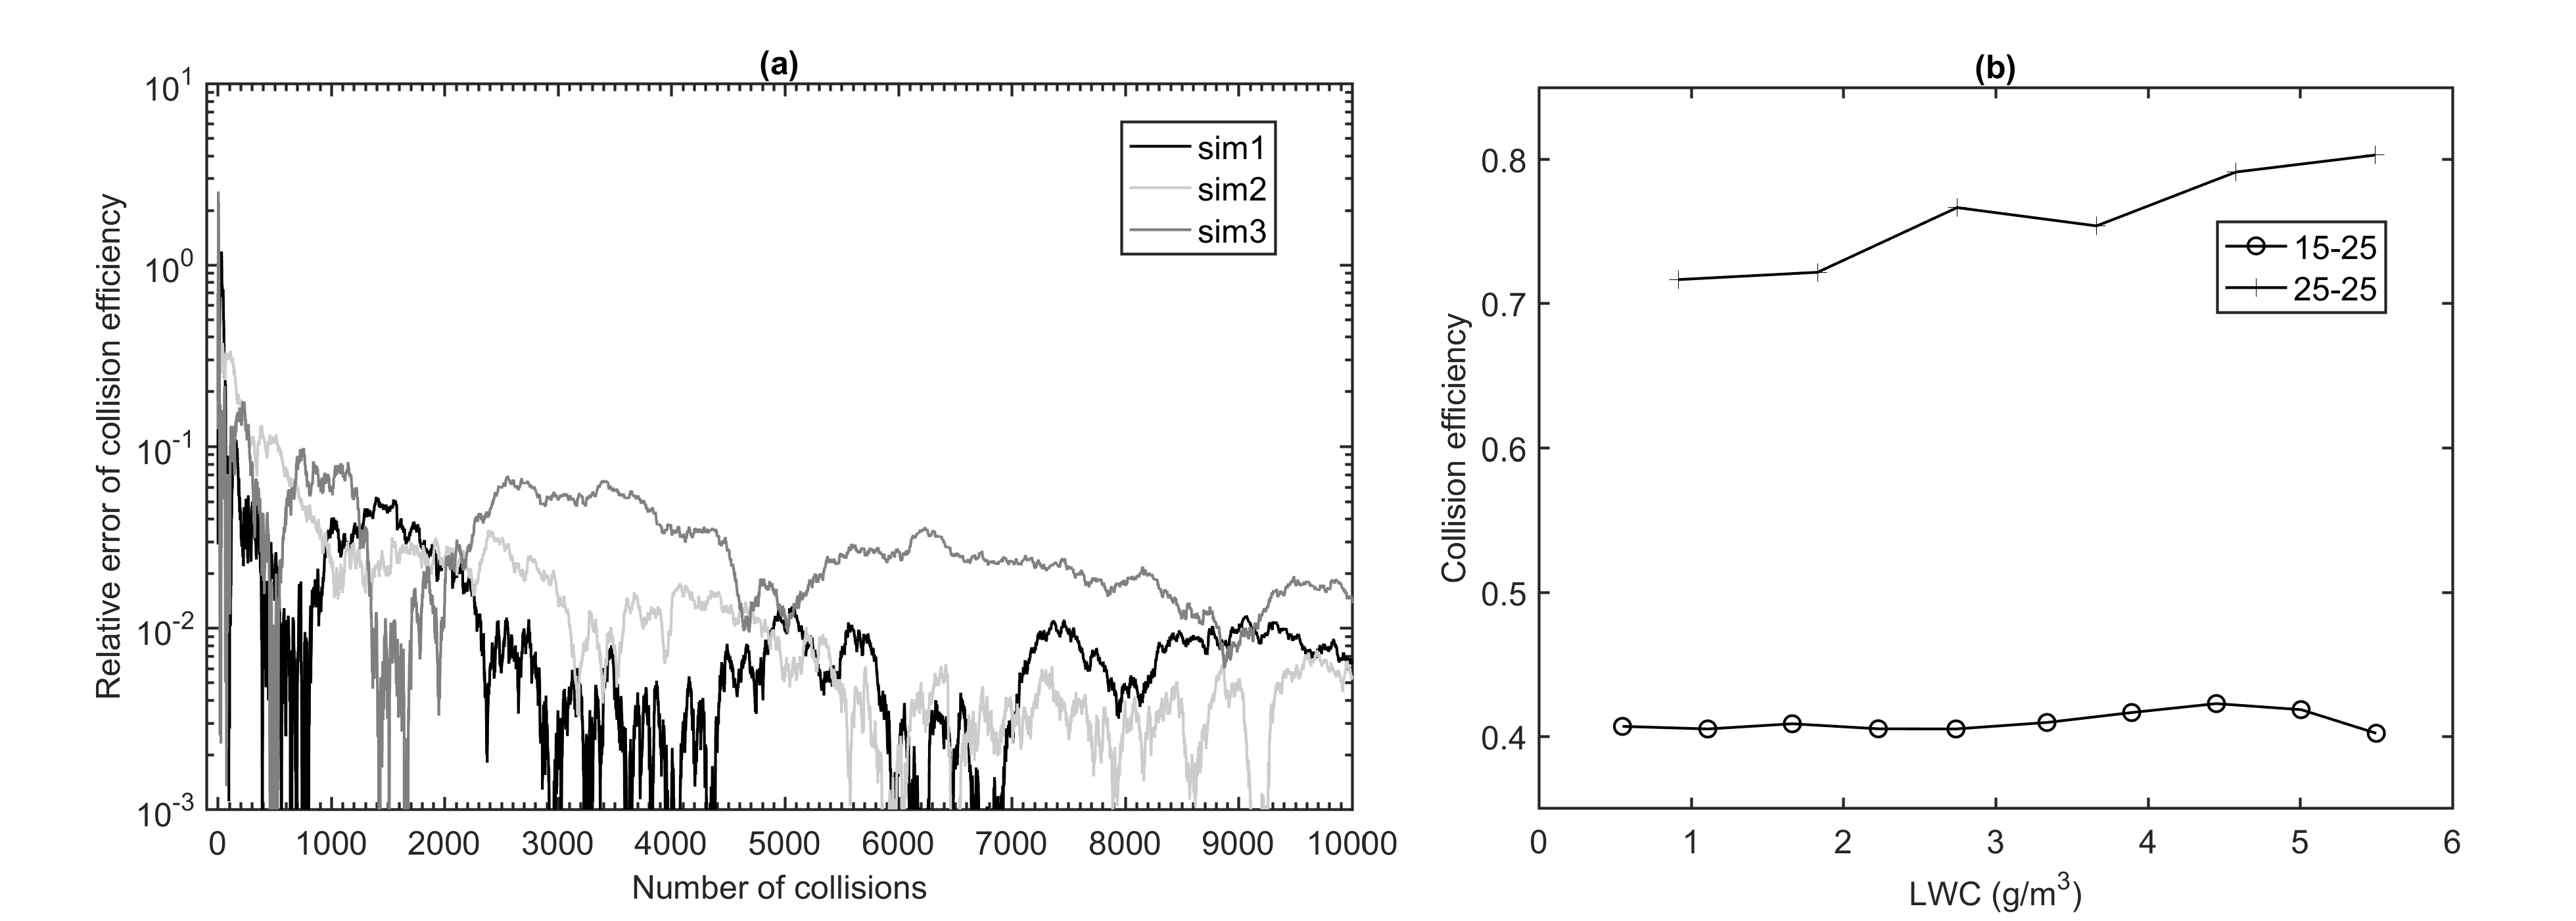
\includegraphics[width=0.8\textwidth]{Figures/Chap3/vali.png}
\caption{(a)Sensitivity test of collision efficiency on the accumulated number of collisions sampled. The $15-25$ $\mu m$ droplet pair is selected to run the simulation. Sim1, sim2, sim3 in the legend denote simulations with different initial droplet locations. (b) Dependency of collision efficiency on the liquid water content (LWC). The droplet pair of $15-25$ $\mu m$ is selected to test the cross-sized collision case and $25-25$ $\mu m$ to test the same-sized collision case. All simulations have a dissipation rate of $500 cm^2s^{-3}$.  } \label{fig:vali}
\end{figure}

The liquid water content (LWC) of all simulations is constrained between 0.1 and 6 $gm^{-3}$, which is a compromise between the droplet size, droplet number concentration, and the typical adiabatic LWCs for cumulus clouds (on the order of 1$gm^{-3}$). \citet{Wang2008} stated that for a system with multiple droplets, collision efficiency not only depends on the disturbance flows by the colliding droplets (near-field pair interaction), but also can be highly impacted by the disturbance flows of surrounding droplets in the system (far-field multi-body interaction) when the droplet mean separation distance is small (i.e., a high LWC). In particular, this impact is more significant for same-sized collisions mainly because the hydrodynamic interaction time between nearly equal-sized droplets are much longer. To investigate the importance of the far-field effect on cross-sized collisions and same-sized collisions, sensitivity tests over the range of LWC are conducted. We choose droplet pairs of 15-25 $\mu m$ for the cross-sized case and 25-25 $\mu m$ for the same-sized case. Simulations with different droplet number concentrations, corresponding to LWC from 0.5 to 5.5 $gm^{-3}$, are performed for both cases  at a dissipation rate of 500 $cm^2s^{-3}$ . The curve of the 15-25 $\mu m$ collision efficiency stays nearly constant, with fluctuations less than 5\% from the mean, showing insignificant influence by the LWCs considered (Fig. \ref{fig:vali}(b)). The same-sized collision efficiency increases slightly with LWC, which agrees with \citet{Wang2008}, but with a smaller increase. We conclude that for cross-sized collision events, far-field effects can be neglected and the collision efficiencies obtained in this study are valid and are applicable to cumulus clouds. In the meantime, caution should be exercised when interpreting same-sized collision results. The LWC values for all mono-disperse cases in this study are listed in table \ref{tab:LWC}.

\begin{table}[ht]
\def\arraystretch{1.5}
\begin{center}
\caption{LWC ($g m^{-3}$) in the monodisperse simulations\strut}\label{tab:LWC}
\begin{tabular}{cccccc}
\hline\hline
\multirow{2}{*}{Droplet size ($\mu m$)} & \multicolumn{5}{c}{$\epsilon$ ($cm^2s^{-3}$)} \\
\cline{2-6}
 & 20 & 50 & 100 & 200 & 500 \\
\hline
10 & 0.106 & 0.105 & 0.178 & 0.298 & 0.586\\
15 & 0.357 & 0.356 & 0.593 & 1.005 & 1.978 \\
20 & 0.423 & 0.844 & 1.406 & 2.383 & 1.875 \\
25 & 0.827 & 1.648 & 2.746 & 4.655 & 5.494 \\
 \hline
\end{tabular}
\end{center}
\end{table}


\section{Result and analysis} \label{sec:ch3_result}


\subsection{Collision efficiency} \label{sec:ch3_reCE}

In this section, four sizes of collector droplets ($r =$ 10, 15, 20, 25 $\mu m$) are investigated, and collision statistics of 28 droplet pair combinations at zero turbulence (Stokes flow simulations) and five turbulence intensities ($\epsilon=$20, 50, 100, 200, 500 $cm^2s^{-3}$) are analyzed. All collision efficiencies are tabulated in the appendix  as they can be applied in the stochastic collision equation or can be used to develop parameterization schemes.

Figure \ref{fig:cer_ratio} demonstrates the variation of collision efficiency with r-ratio, defined as the radius ratio of collected and collector droplet ($r_1/r_2$). For a brief comparison with previous studies, we mention that similar trends are observed among our curves and the results from \citet{Pinsky2008} and \citet{Wang2008}. In particular, our collision efficiency quantitatively agrees well with \citet{Pinsky2008} for most cases while slightly greater for $r_2=20$ $\mu m$ when $r_1/r_2 < 0.7$. However, greater values are observed in \citet{Wang2008}. This difference can be caused partially by the possible overestimation of far-field aerodynamical interaction in their case due to the high LWCs and partially by the different fluid parameters ($\nu$, $\rho_d$, $\rho_a$, etc.) chosen to calculate droplet terminal velocity. Overall, the collision efficiency shows convergence at weak turbulence and increases with dissipation rate. \citet{Wang2008} found that, for cross-sized collisions, collision efficiency exhibits a strongly positive correlation to the reduction of droplet relative velocity, due to the presence of the disturbance flow. The turbulence enhancement of collision efficiency is mainly because the disturbance flow becomes less effective in reducing the droplet relative velocity when turbulence is present. We can extrapolate that as turbulence continues to intensify, the influence of the disturbance flow diminishes and the collision kernel converges to the geometric collision kernel at a different rate for various r-ratios.  


\begin{figure}[ht]
\centering
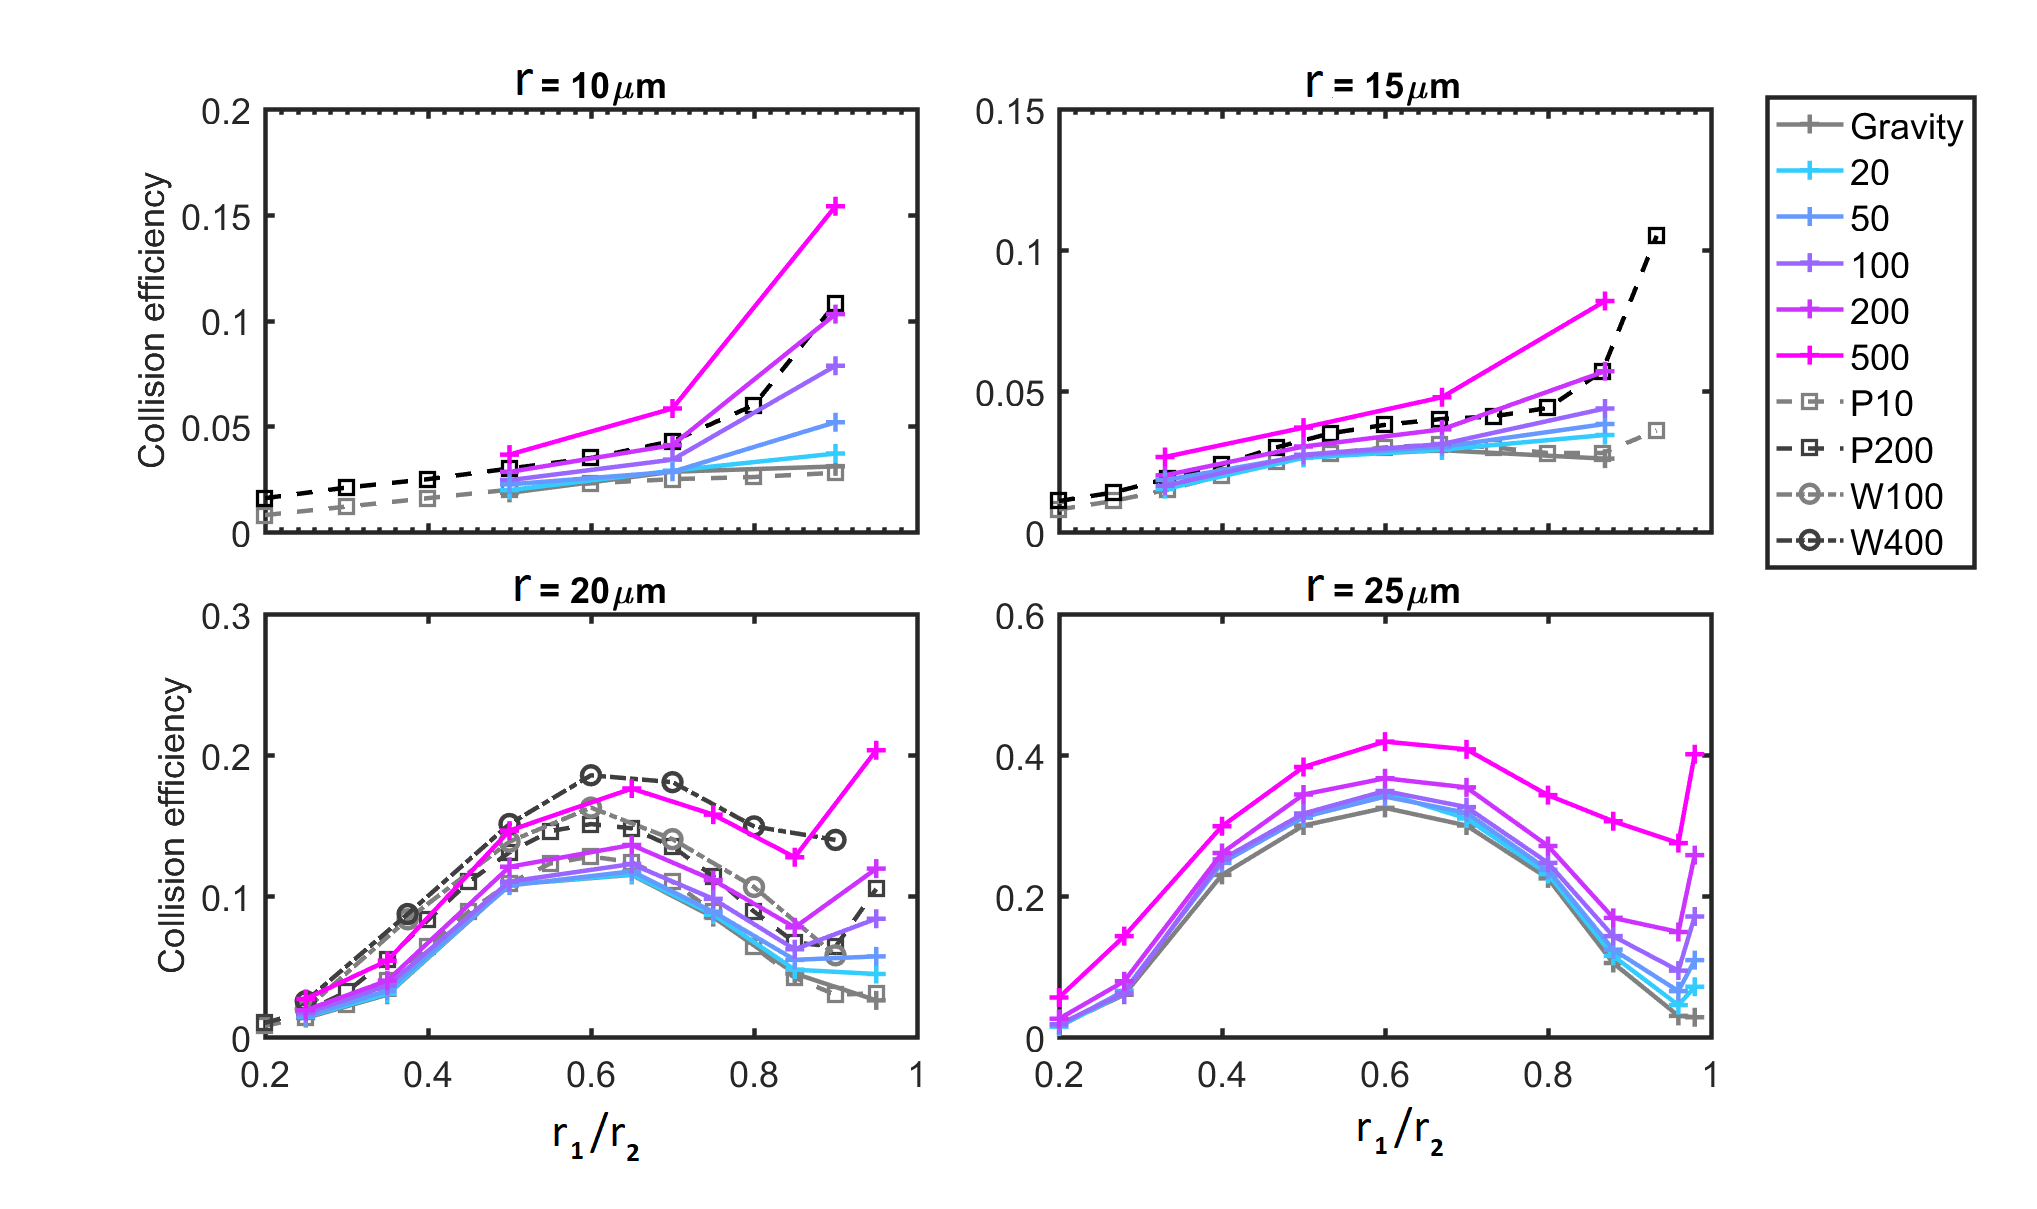
\includegraphics[width=0.8\textwidth]{Figures/Chap3/cer_ratio.png}
\caption{Collision efficiency for different collector droplets as a function of r-ratio at different turbulent environments for four different sizes of collector droplets (shown in the title of each panel). Colors demarcate dissipation rates with corresponding values  (in $cm^2s^{-3}$) shown in the legend. Collision efficiency from \citet{Pinsky2008} (dashed line with squares) and \citet{Wang2008} (dashed line with circles) are shown for comparison with dissipation rates listed in the legend. The collision efficiency of \citet{Wang2008} is produced from the multiplication of the enhancement factor from their table B.4. and gravitational collision efficiency from \citet{Wang2005a}. } \label{fig:cer_ratio}
\end{figure}

To examine how turbulence enhancement varies with r-ratio, we calculate the enhancement factor, which is defined as the collision efficiency normalized by its gravitational value. Figure \ref{fig:enhance} shows the enhancement factor of the four collector droplets at the dissipation rate of $\epsilon = 200 cm^2s^{-3}$. As can be seen, the trend is consistent with the enhancement calculated from \citet{Pinsky2008} at $\epsilon = 200 cm^2s^{-3}$ and \citet{Wang2008} at $\epsilon = 100 cm^2s^{-3}$. Enhancement is greatest for similar-sized collisions, indicating that turbulence has its strongest influence in modifying the hydrodynamic interactions between droplets of similar sizes. The enhancement is very weak and stays below 1.5 for $0.2 < r_1/r_2 < 0.8$. According to \citet{Pinsky2008} (purple dashed line in the figure), the enhancement at small r-ratio ($r_1/r_2 < 0.2$) has a comparably large magnitude with the similar-sized case, i.e., collisions containing tiny droplets. However, the collision efficiency of those minuscule droplets remains tiny even after the inclusion of the turbulence effect. This is mainly because tiny droplets tend to follow the flow due to their small inertia. Therefore, turbulence effects make their largest contribution in altering the collision rates between similar-sized droplets. Another intriguing finding is that the enhancement is highly sensitive to the r-ratio but weakly dependent on the size of collector droplets given a fixed r-ratio. This indicates a potential simplification in future parameterizations of the turbulent enhancement of collision efficiency for droplets less than 25 $\mu m$, as those sizes are crucial to initiating effective gravitational collisions. However, it is noteworthy that this feature does not hold for larger droplets. As shown by \citet{Wang2008}, the enhancement weakens as the collector droplet reach 30 $\mu m$ and beyond. 


\begin{figure}[ht]
\centering
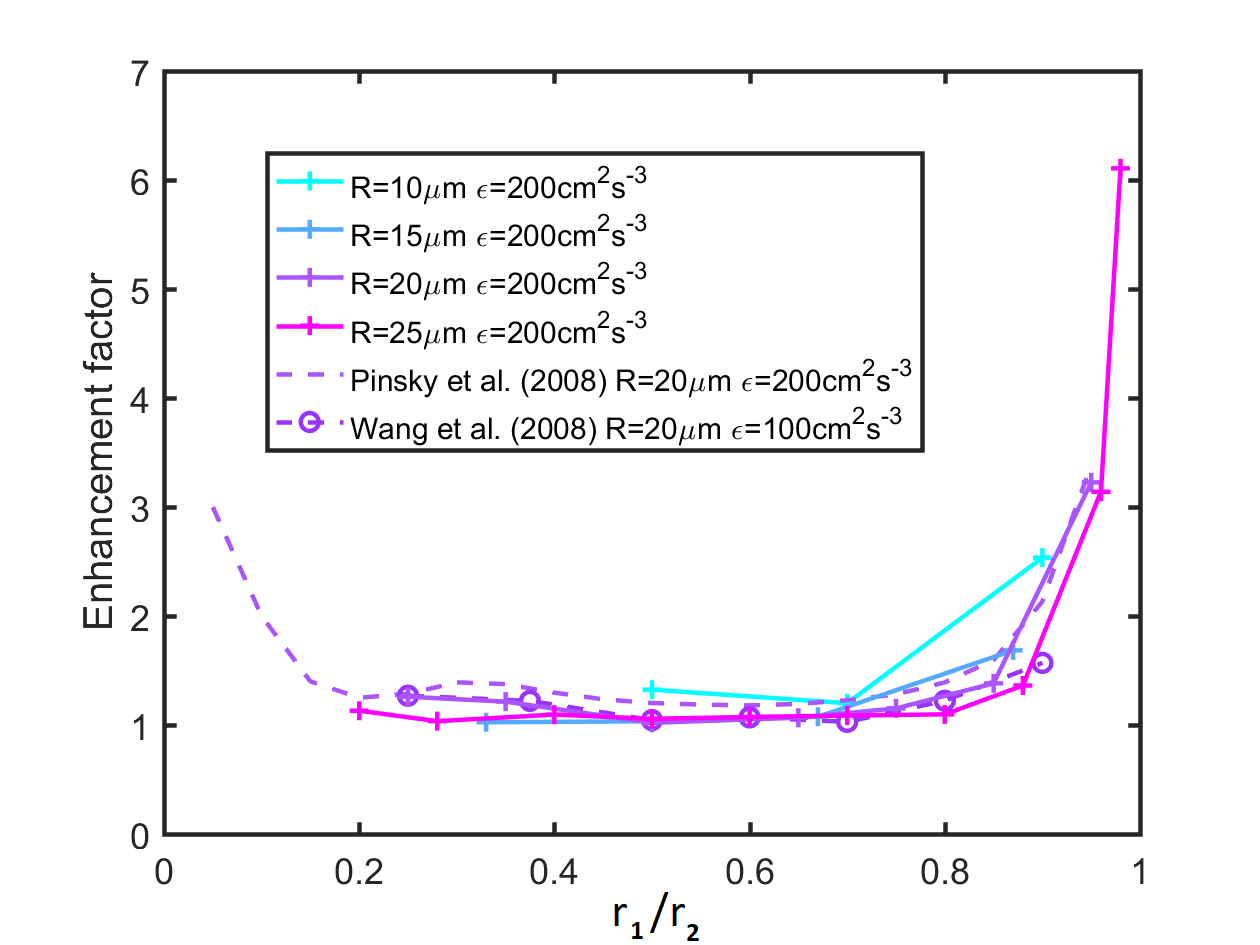
\includegraphics[width=0.8\textwidth]{Figures/Chap3/enhance.png}
\caption{ Turbulence enhancement factor of collision efficiency for all four collector droplets at dissipation rate of 200 $cm^2s^{-3}$ (shown in solid lines with cross markers). Enhancement factor of $r_2 = 20$ $\mu m$ from \citet{Wang2008} at $\epsilon = 100 cm^2s^{-3}$ with Reynolds number of 72.4 and from \citet{Pinsky2008} at $\epsilon = 200 cm^2s^{-3}$ are shown for comparison.} \label{fig:enhance}
\end{figure}


The same-sized collision efficiency remains close to unity but decreases slightly with dissipation rate (Fig. \ref{fig:samesize}(a) ). This has also been reported by \citet{Wang2008} in some cases. However no conclusive explanation was given due to the high uncertainty in their data. A possible explanation for the decrease can be found by studying the statistics of the radial relative velocity (RRV) and the radial distribution function (RDF), owing to the fact that the disturbance flow affects collision efficiency mainly by influencing the droplet relative motion and altering the droplet clustering within its effective range. RRV is the radial component of the relative velocity of colliding droplets. Its mean value is calculated via $\langle |\mathbf{W}_r | \rangle = \left\langle \left| \mathbf{W} \cdot \frac{\mathbf{d}}{|\mathbf{d}|} \right| \right\rangle $ with $\mathbf{W}$ being the droplet relative velocity and $\mathbf{d}$ being the separation vector. RDF measures the droplet clustering and is defined by $g(R)=\frac{N_p \Omega}{V_s N_t N_1 N_2}$. $N_p$ is the number of droplet pairs at contact found in the shell of collision sphere within $N_t$ time steps. The shell volume $V_s=\frac{4\pi}{3} [(1.01\times R)^3-R^3]$ has an outer radius slightly larger than the sum of droplet radii for sufficient sampling at finite $N_t$, which is safe to do so as long as the outer radius is smaller than $1.1 \times R$ \citep{Wang2000}. Because the non-overlapping treatment alters the mean RRV and the symmetry of the droplet radial distribution at contact, corrections for both RRV and RDF should be included to achieve the correct kinematic properties \citep{Wang2005b}, i.e., $\langle |\mathbf{W}_r|\rangle^{cor}=\langle|\mathbf{W}_r |\rangle \times C_w$, and $g(R)^{corr}=g(R)\times C_g$. $C_w$ and $C_g$ are determined by the shell thickness of the collision sphere and their expressions are provided in \citet{Wang2005b}.

Figure \ref{fig:samesize}(b) displays the normalized mean RRV of four same-sized droplet pairs varying with dissipation rates. The normalization is made by taking the ratio of RRV in the DF case and the corresponding value in the nonDF case. Similar to the collision efficiency curves in panel (a), RRV also demonstrates a decaying trend with intensifying turbulence. A weak decay is also found in the normalized RDF (panel (c) in Fig. \ref{fig:samesize}), consistent with panel (a) and (b) in spite of the larger fluctuations compared to the former two statistics. It seems that the turbulence effect in counteracting the droplet disturbance flow weakens as the turbulence intensifies, regardless of the fact that the RRVs and RDFs in both DF and NonDF runs increase with eddy dissipation rate (not shown). 

\begin{figure}[ht]
\centering
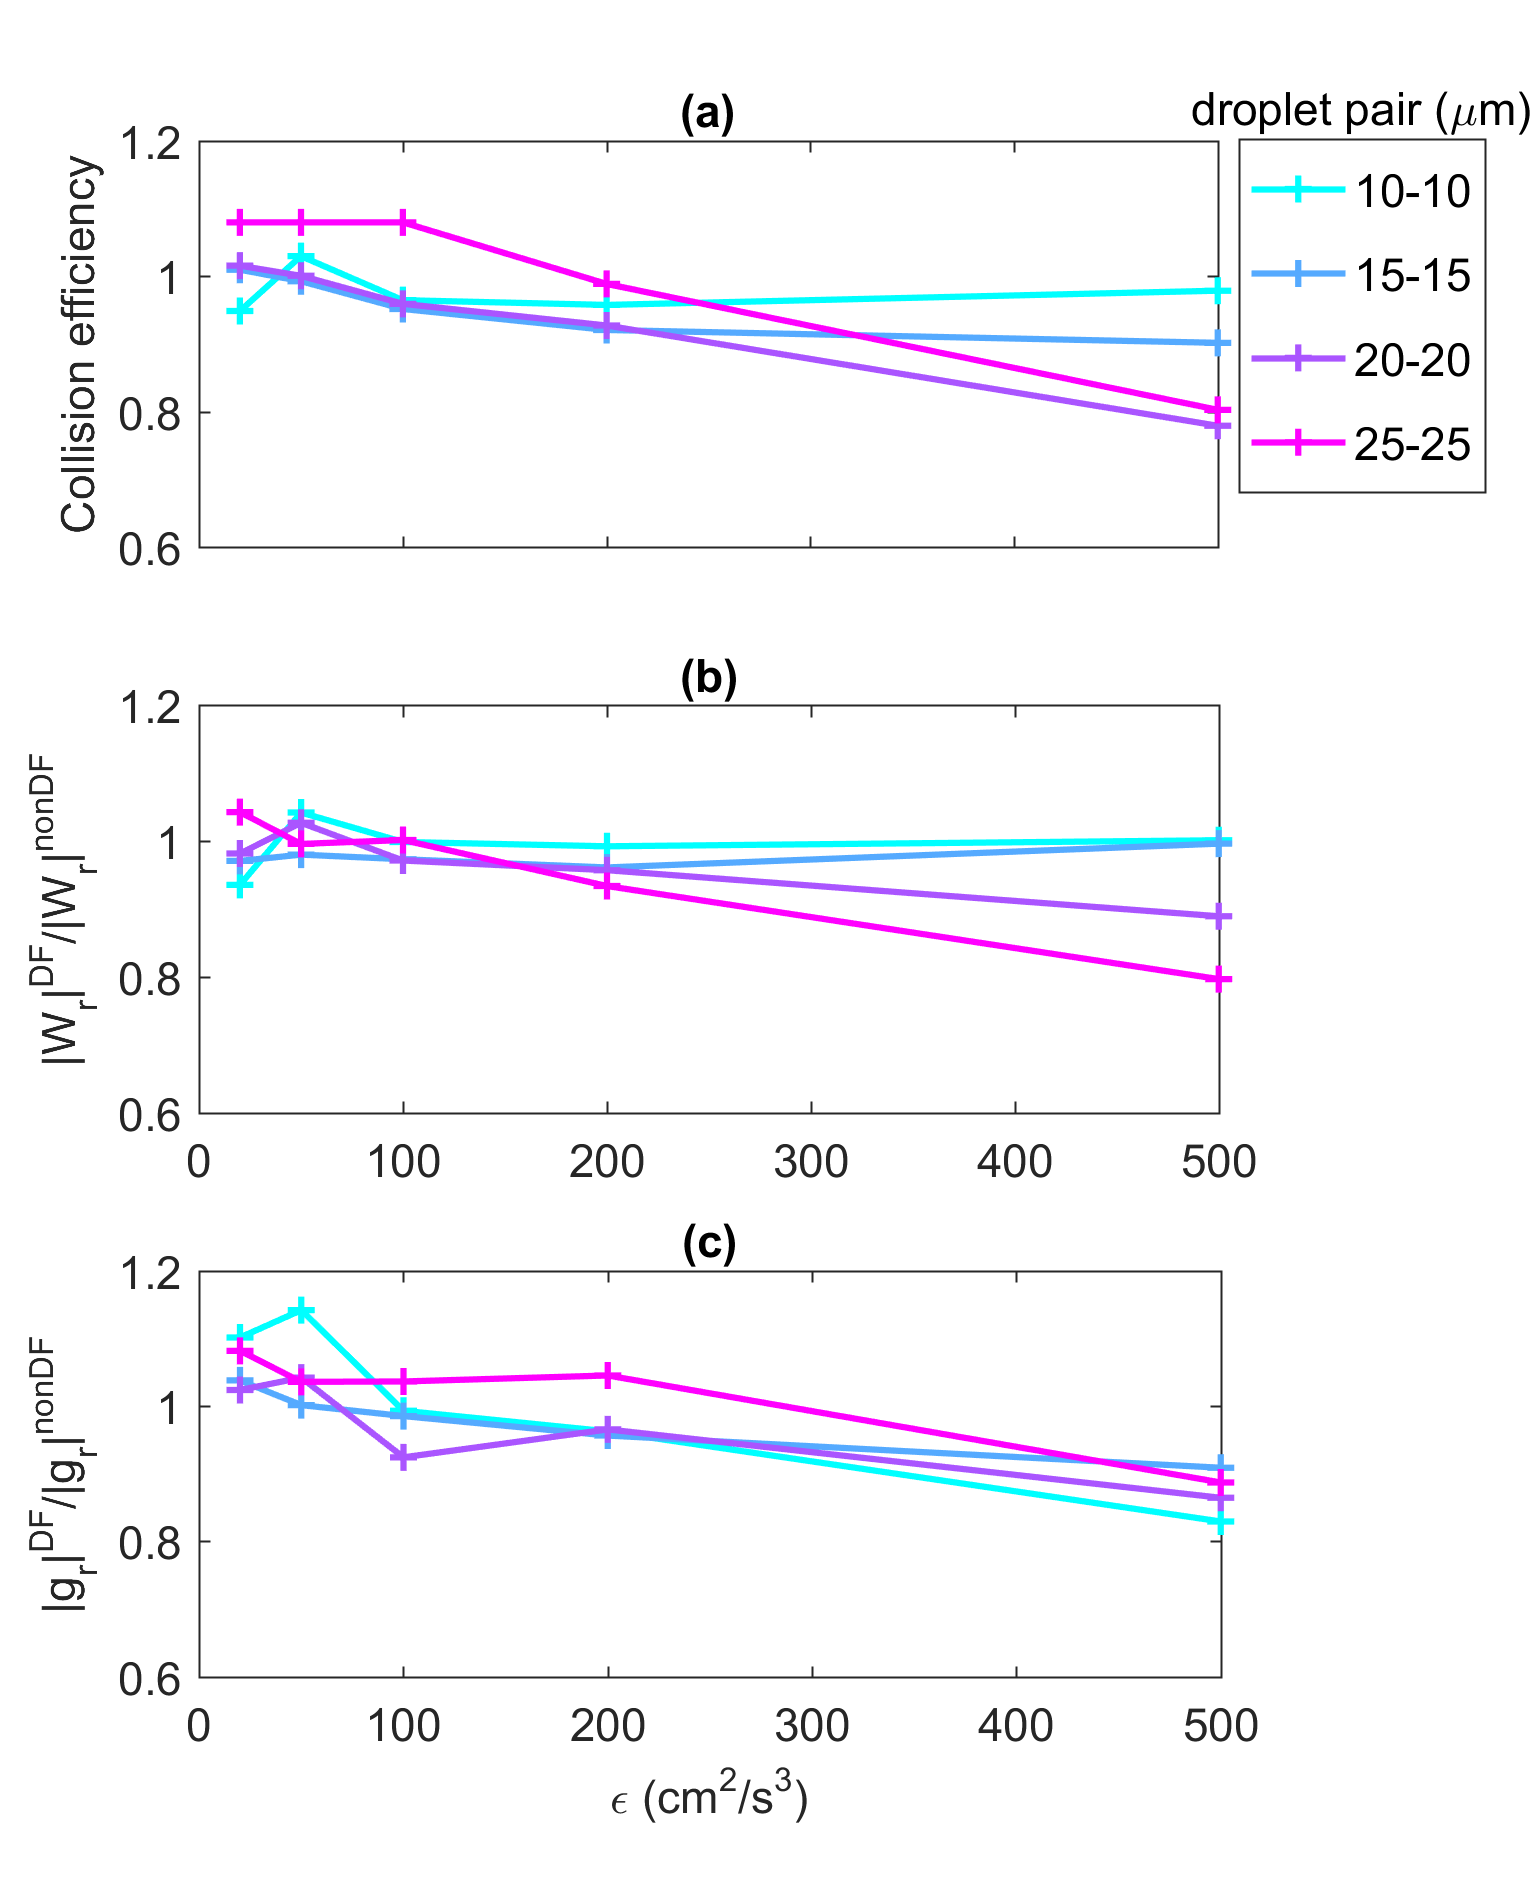
\includegraphics[width=0.8\textwidth]{Figures/Chap3/samesize.png}
\caption{Same-sized collision statistics of (a) Collision efficiency, (b) Normalized radial relative velocity in DF case by nonDF case, and (c) normalized radial distribution function as function of dissipation rate for four different droplet sizes. The normalization in panel (b) (panel (c)) is made by taking the ratio of RRV (RDF) in the DF case and the corresponding value in the nonDF cases. } \label{fig:samesize}
\end{figure}


\subsection{Turbulent collision kernel} \label{sec:ch3_reTCK}

The turbulence enhancement of the geometric collision kernel is relatively weak in a mildly turbulent environment \citep{Ayala2008a, Chen2016}. As Fig. \ref{fig:tgck} shows, the geometric collision kernel at all turbulence intensities peaks at intermediate r-ratios and drops to its lowest at same-sized collisions. However, after taking into account the collision efficiency, the curves display a very different pattern (Fig. \ref{fig:tck}) and a significant enhancement of the collision kernel in similar-sized collisions is observed. Even though the same-sized droplet pairs have much smaller geometric collision kernels (Fig. \ref{fig:tgck}), their high collision efficiency in mild to strong turbulence moves the collision kernel to a comparable magnitude as in the intermediate r-ratio regime. For small collector droplets ($r_2 = 10$ $\mu m$), the peak at r-ratio$\sim 0.6$ disappears and the collision kernel maximizes at similar-sized droplet pairs when $\epsilon > 100$ $cm^2s^{-3}$, in agreement with \citet{Pinsky2008} (see the black dashed line in the first panel of Fig. \ref{fig:tgck}). As shown in Chapter \ref{sec:ch2}, turbulence causes a very pronounced enhancement of the local clustering and relative motion in similar-sized droplet pairs, and thus greatly increases their geometric collision kernel. In this paper, we find that the turbulence enhancement of the collision efficiency is also most intense for comparable-sized pairs. The above two factors consolidate a much stronger enhancement of collision kernel for similar-size pairs. The implication is that, as the condensational growth rate slows down as droplets get larger and concurrently narrows the size spectra, turbulence can boost the broadening process through efficient similar-sized collisions and accelerate the collisional growth.

\begin{figure}[ht]
\centering
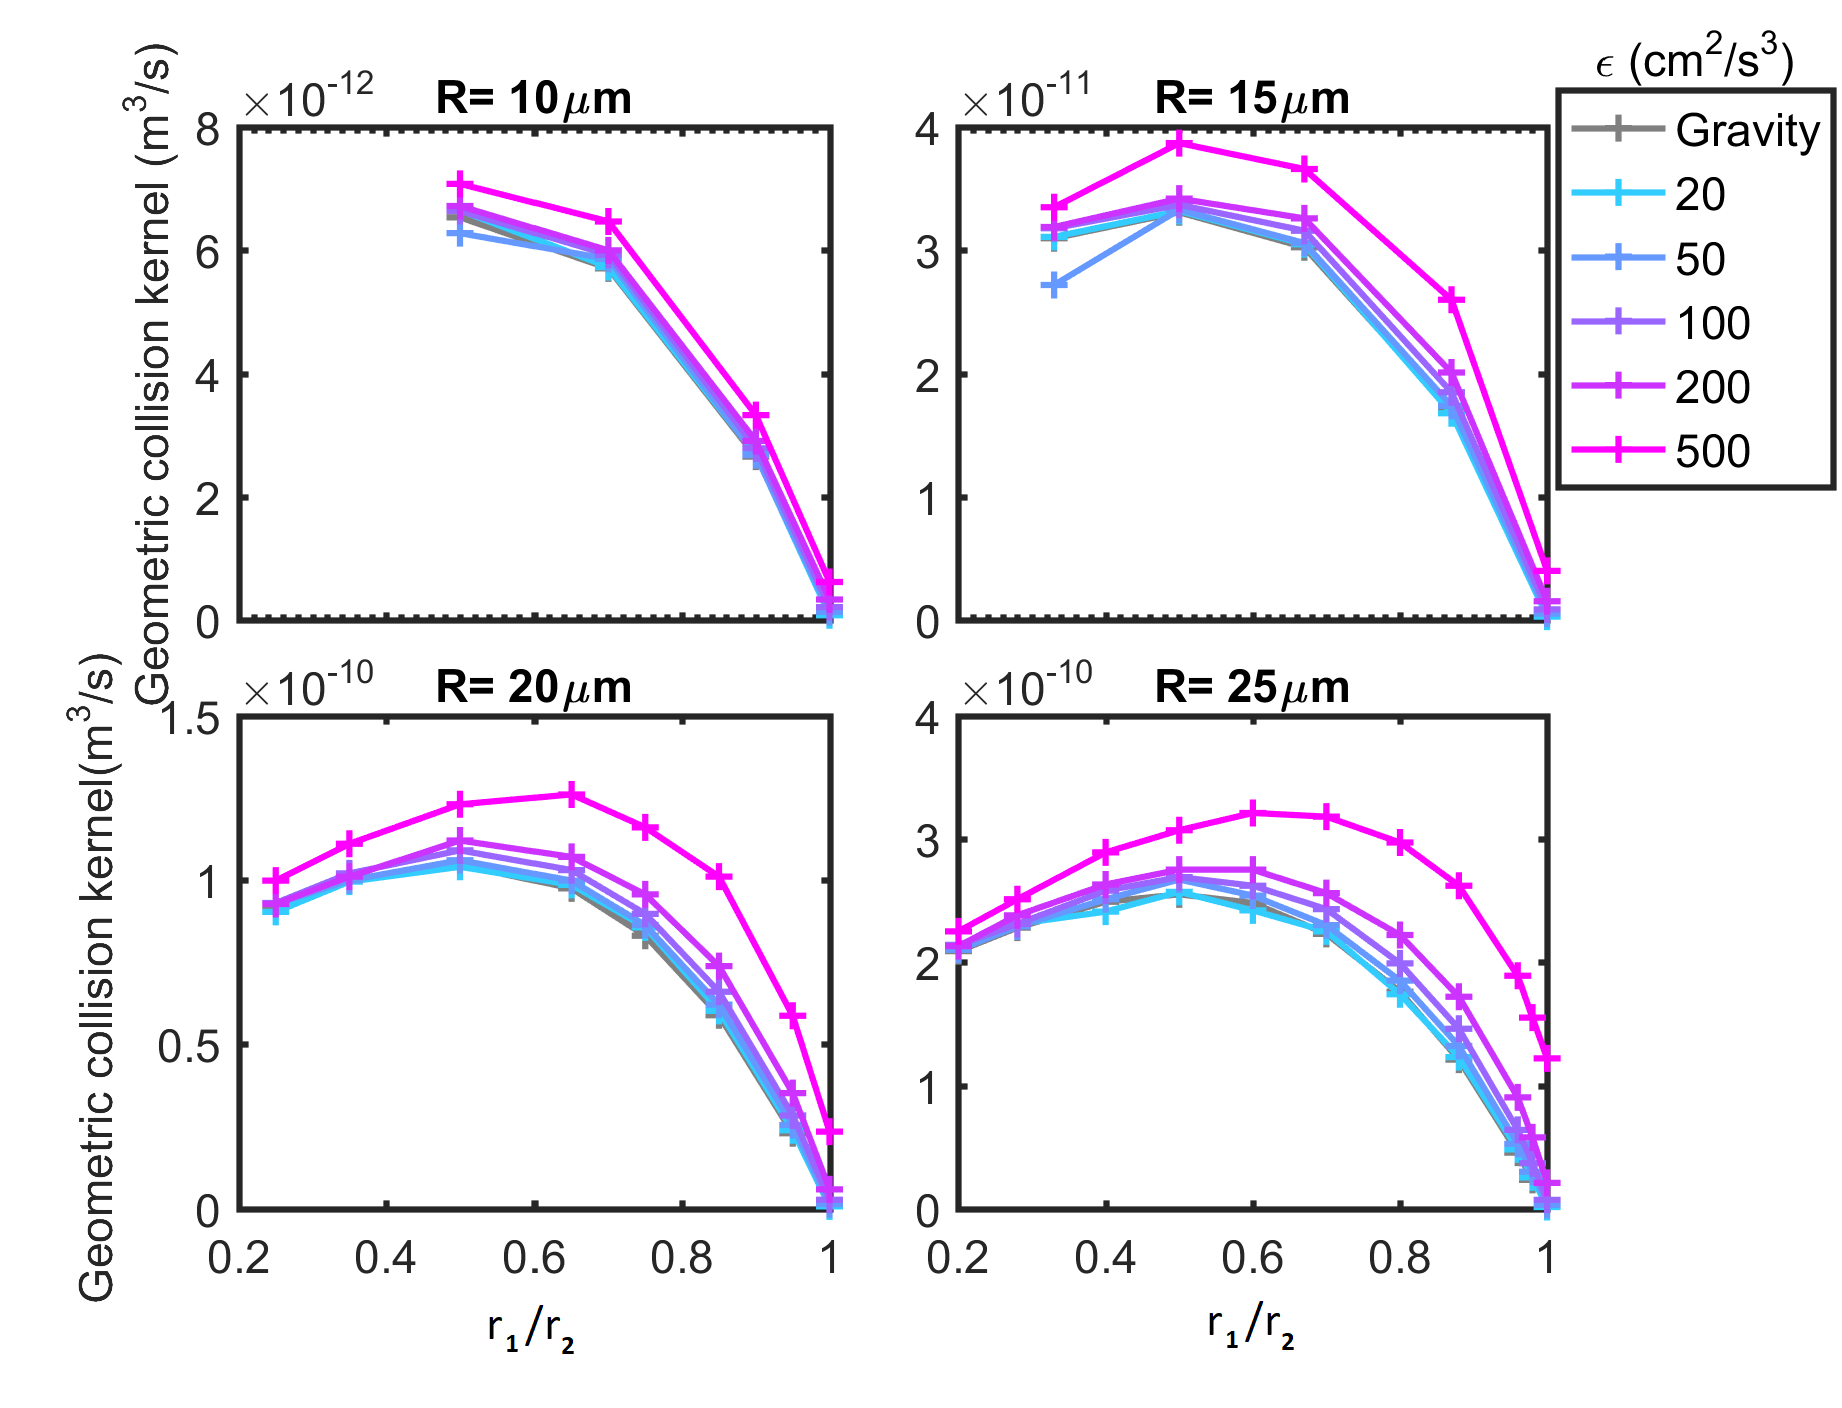
\includegraphics[width=0.8\textwidth]{Figures/Chap3/tgck.png}
\caption{Same as Fig. \ref{fig:cer_ratio} but for the turbulent geometric collision kernel ($m^3s^{-1}$).} \label{fig:tgck}
\end{figure}

\begin{figure}[ht]
\centering
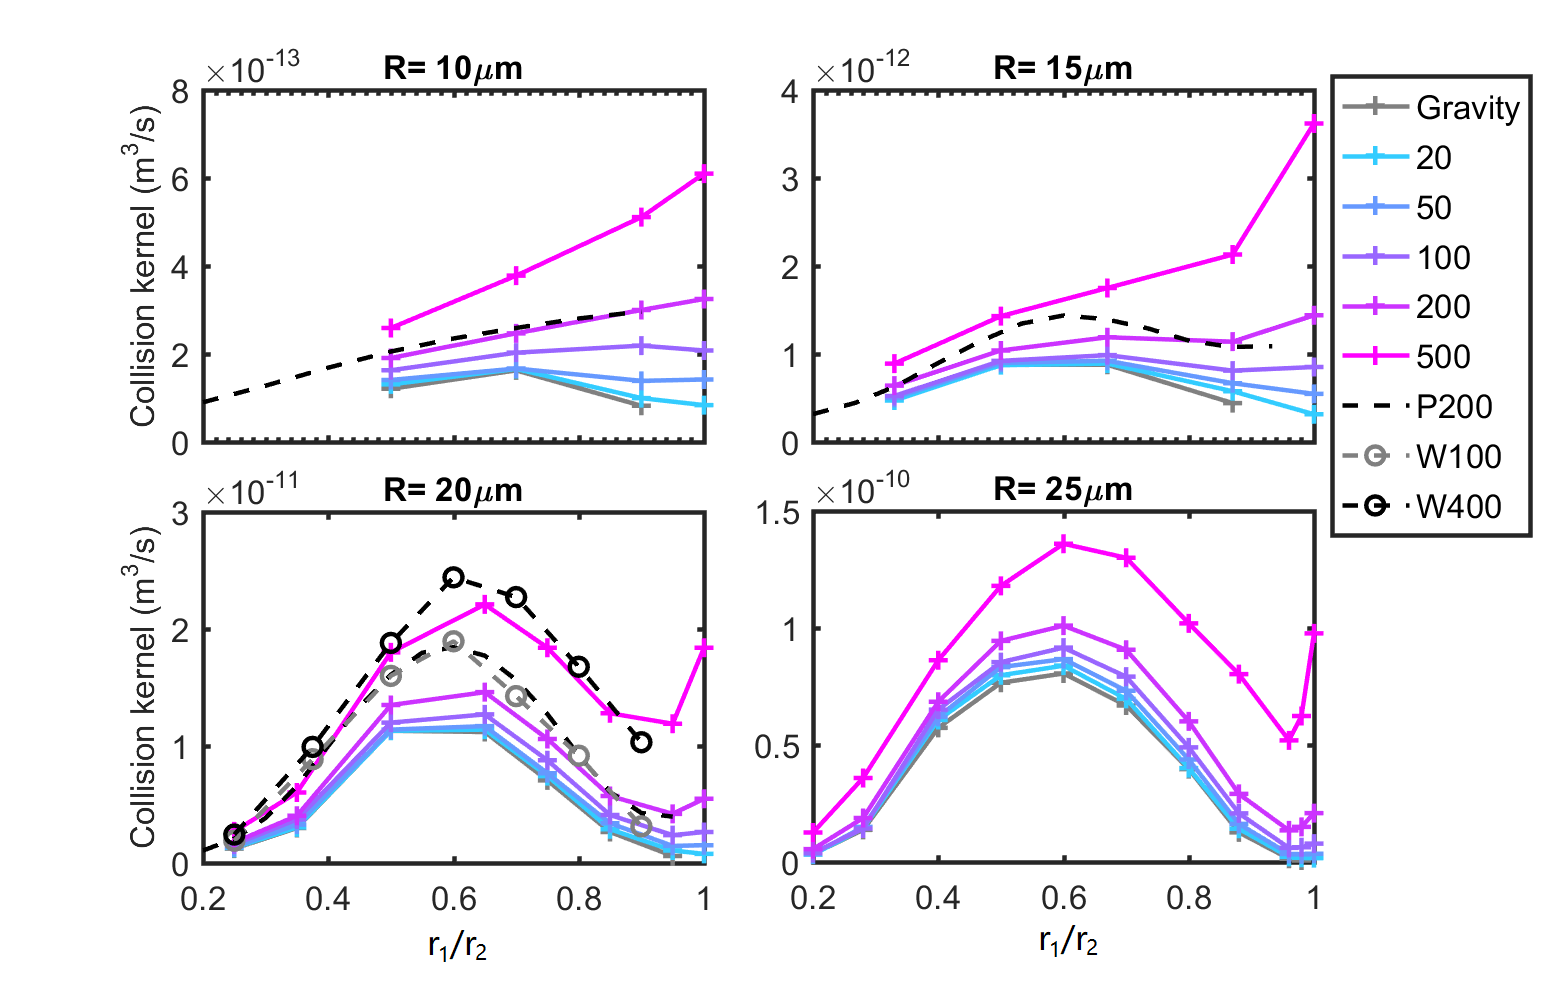
\includegraphics[width=0.8\textwidth]{Figures/Chap3/tCK.png}
\caption{same as Fig. \ref{fig:cer_ratio} but for the turbulent collision kernel ($m^3s^{-1}$). Collision kernel of $r_2 = 20$ $\mu m$ from \citet{Wang2008} at $\epsilon=100$ $cm^2s^{-3}$ and $\epsilon=400$ $cm^2s^{-3}$ with Reynolds number of 72.4 (dashed lines marked with circles and labeled as "W100" and "W400" in the legend) and from \citet{Pinsky2008} with $\epsilon=200$ $cm^2s^{-3}$ are shown for comparison (dashed lines labeled with "P200"). Dissipation rates are listed in the legend.} \label{fig:tck}
\end{figure}

\subsection{Evolution of droplet size distribution} \label{sec:ch3_reDSD}

To illustrate the turbulence broadening hypothesis in the last section, we conduct simulations that allow droplets to grow by collision-coalescence to investigate the impact of turbulence on DSD evolution. 

The initial shape of DSD (green dashed lines in Fig. \ref{fig:DSD}) is adopted from an aircraft observation through cumulus clouds off the coast of Hawaii \citep{Raga1990}. LWC is fixed at a typical adiabatic value of 1 $gm^{-3}$. Four dissipation rates are investigated ($\epsilon$ = 50, 100, 200, and 500 $cm^2s^{-3}$) and this range covers the most frequently observed turbulent environments observed in cumulus and stratocumulus clouds. A simulation without turbulence will also be performed for comparison. We run each simulation for 6.5 minutes of real time and observe the time evolution of the DSD. To reduce the impact of initial conditions in the pure-gravity case, three ensemble runs with different initial droplet locations are performed, and the mean value of the three realizations is used in the analysis.

Figure \ref{fig:DSD} depicts the droplet size spectra and mass density spectra at the end of the simulations. The discontinuous tails of the distributions result from the few large droplets formed in the domain. While broadening of the spectrum in the form of an exponential tail occurs in all experiments, the broadest spectrum is observed at our strongest turbulence. The number and mass of large droplets ($r > 20$ $\mu m$) for the gravity case stays lowest among the five simulations. Figure \ref{fig:timeDSD} shows the DSD evolution of the same five simulations. Droplet number concentrations below 0.001 $cm^{-3}$ are treated as statistical uncertainty since they correspond to less than 2-3 droplets in the domain, and thus there is no color in the plot. As expected, the DSD of the pure gravitational case stays relatively narrow throughout the simulation (panel (a) of Fig. \ref{fig:timeDSD}).) and droplets larger than 30 $\mu$m remain "invisible". In comparison, droplets grow larger than 35 $\mu$m at the end of all simulations with turbulence(see the purple colored edge in \ref{fig:timeDSD}). This again indicates that even weak turbulence plays an efficient role in DSD broadening and produces a considerable number of large droplets. As dissipation rate continues to increase, the distribution tail expands at a faster pace. In the case with $\epsilon=500$ $cm^2s^{-3}$, droplets larger than 45 $\mu$m can be visible at the end and the largest droplet reaches 68 $\mu$m. 

\begin{figure}[ht]
\centering
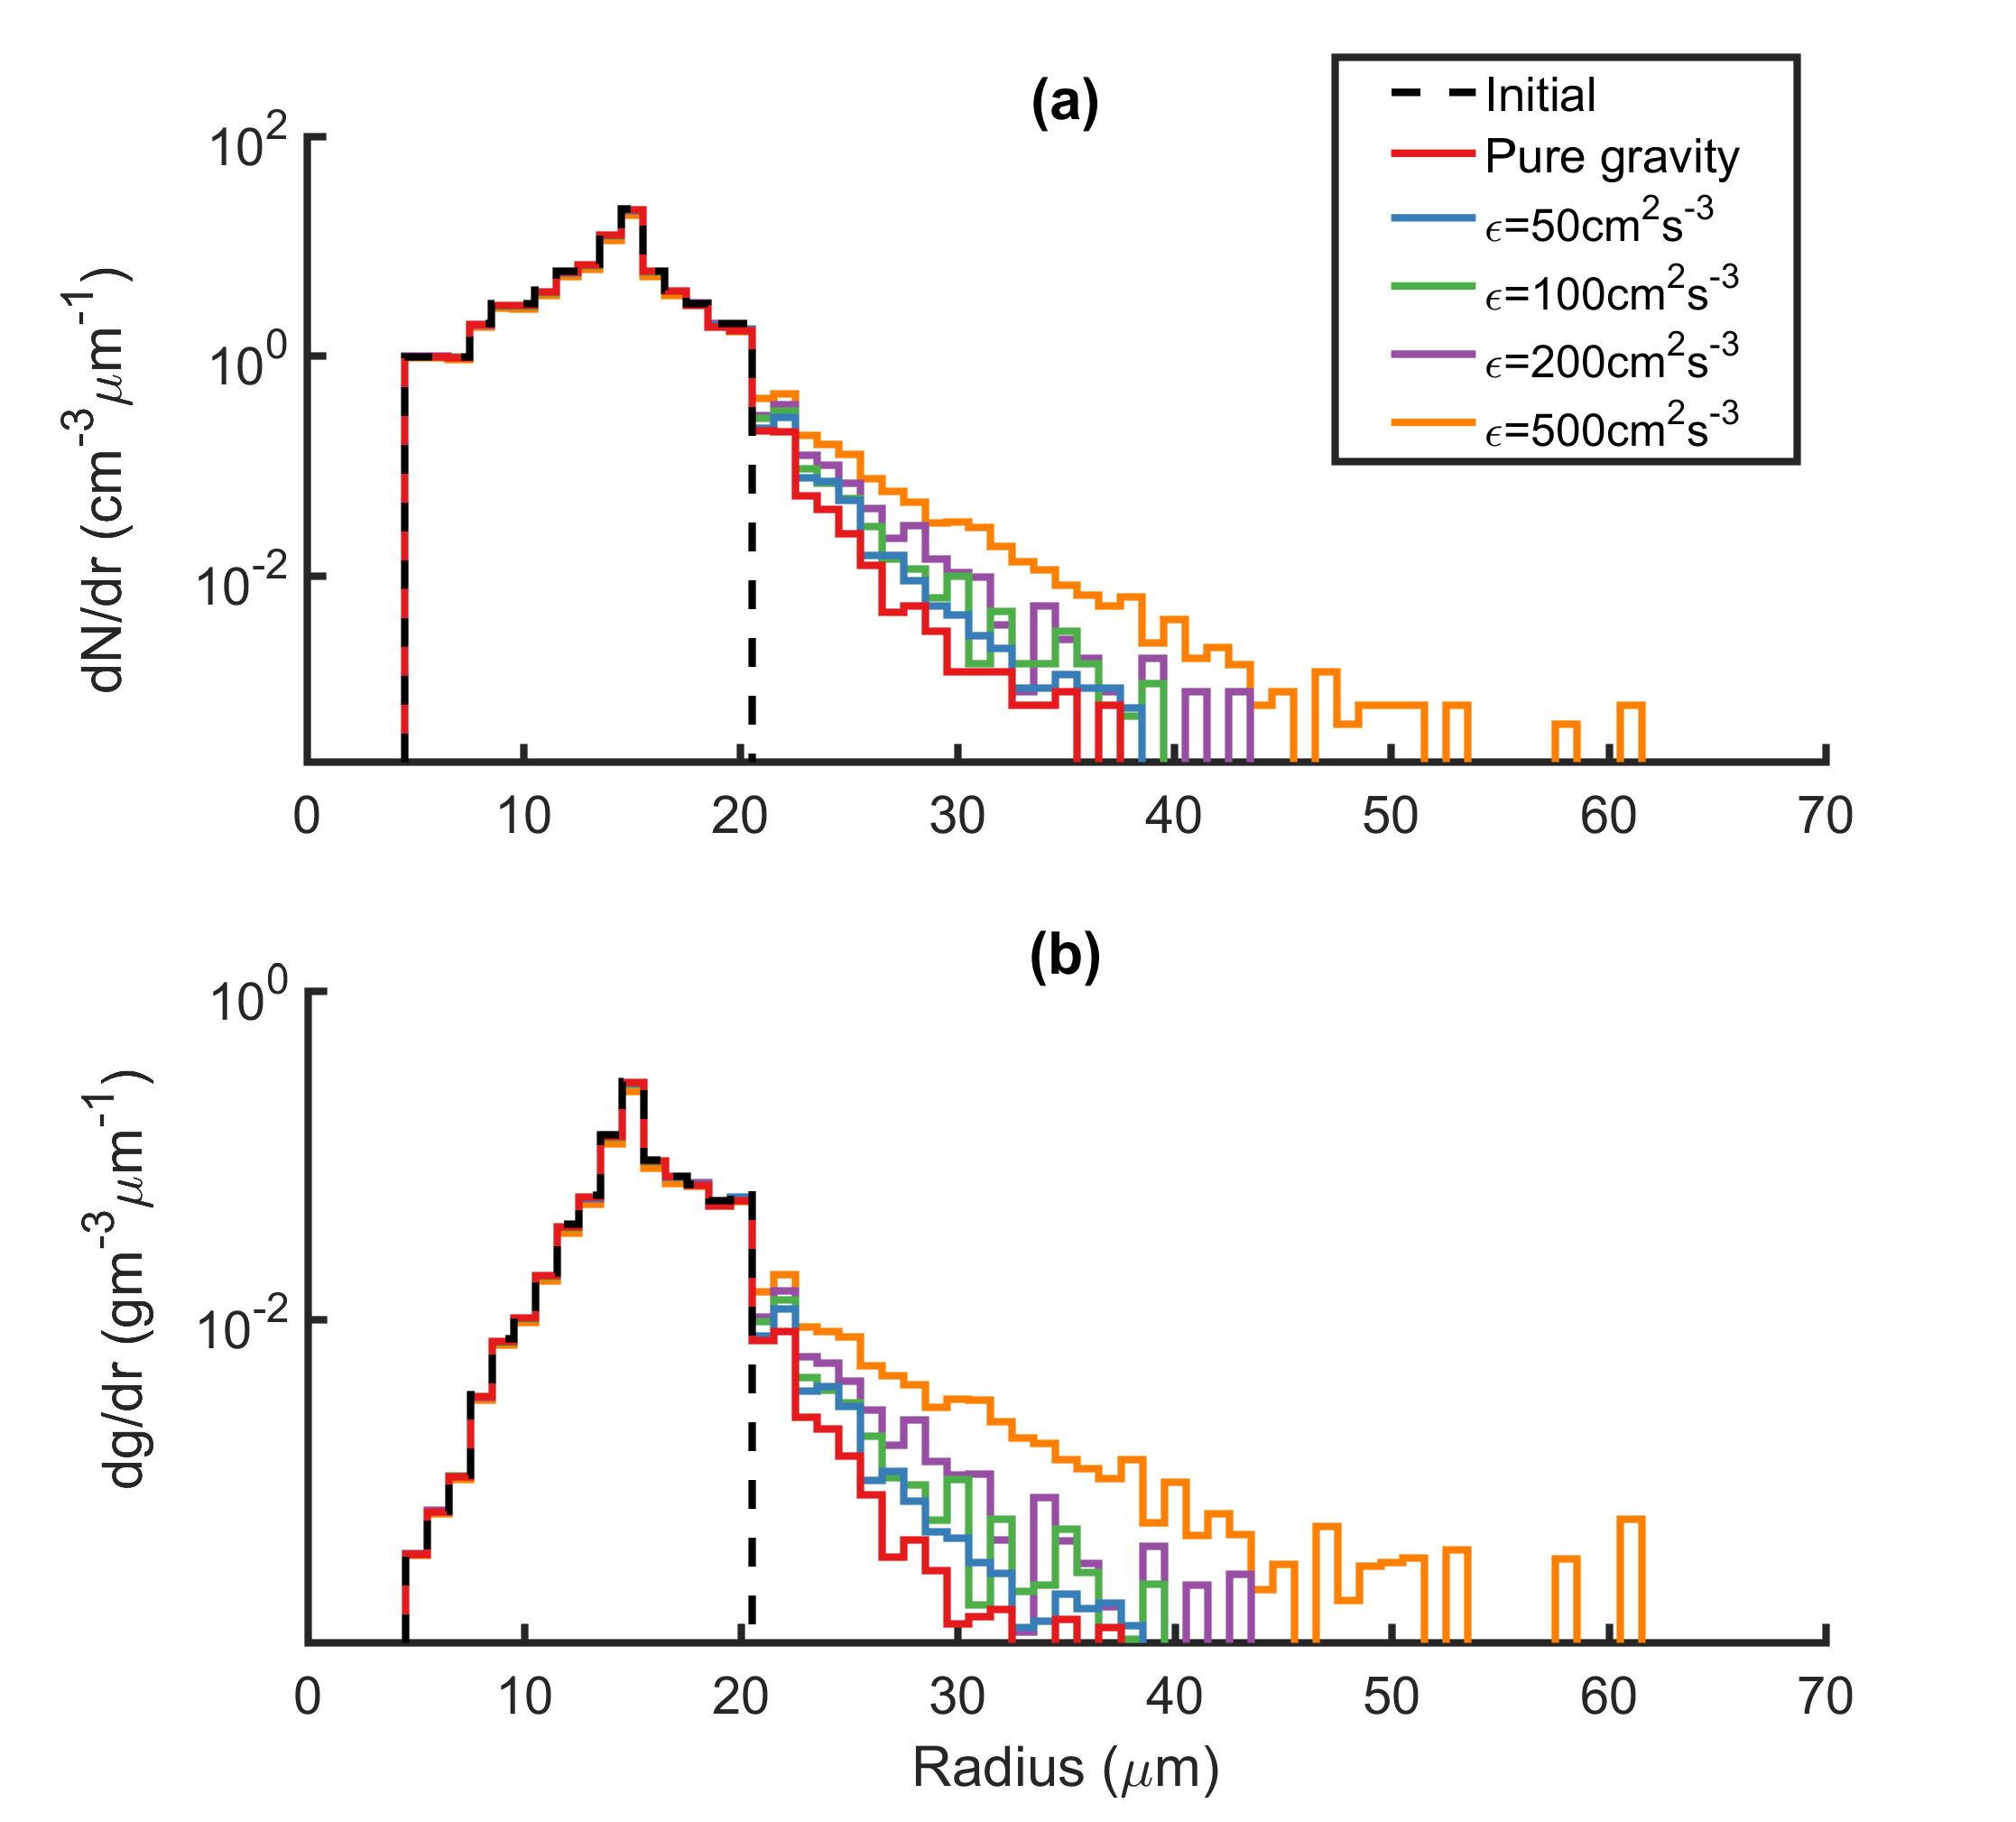
\includegraphics[width=0.8\textwidth]{Figures/Chap3/DSD.png}
\caption{(a) Droplet size distribution and (b) mass density distribution at the 6.5th minute in five different turbulence environments ($\epsilon=0, 50, 100, 200, 500$ $cm^2 s^{-3}$). The initial DSD (black dashed line) is adopted from the flight observation \citet{Raga1990}. LWC is kept 1 $g/m^3$ for all simulations.} \label{fig:DSD}
\end{figure}

\begin{figure}[ht]
\centering
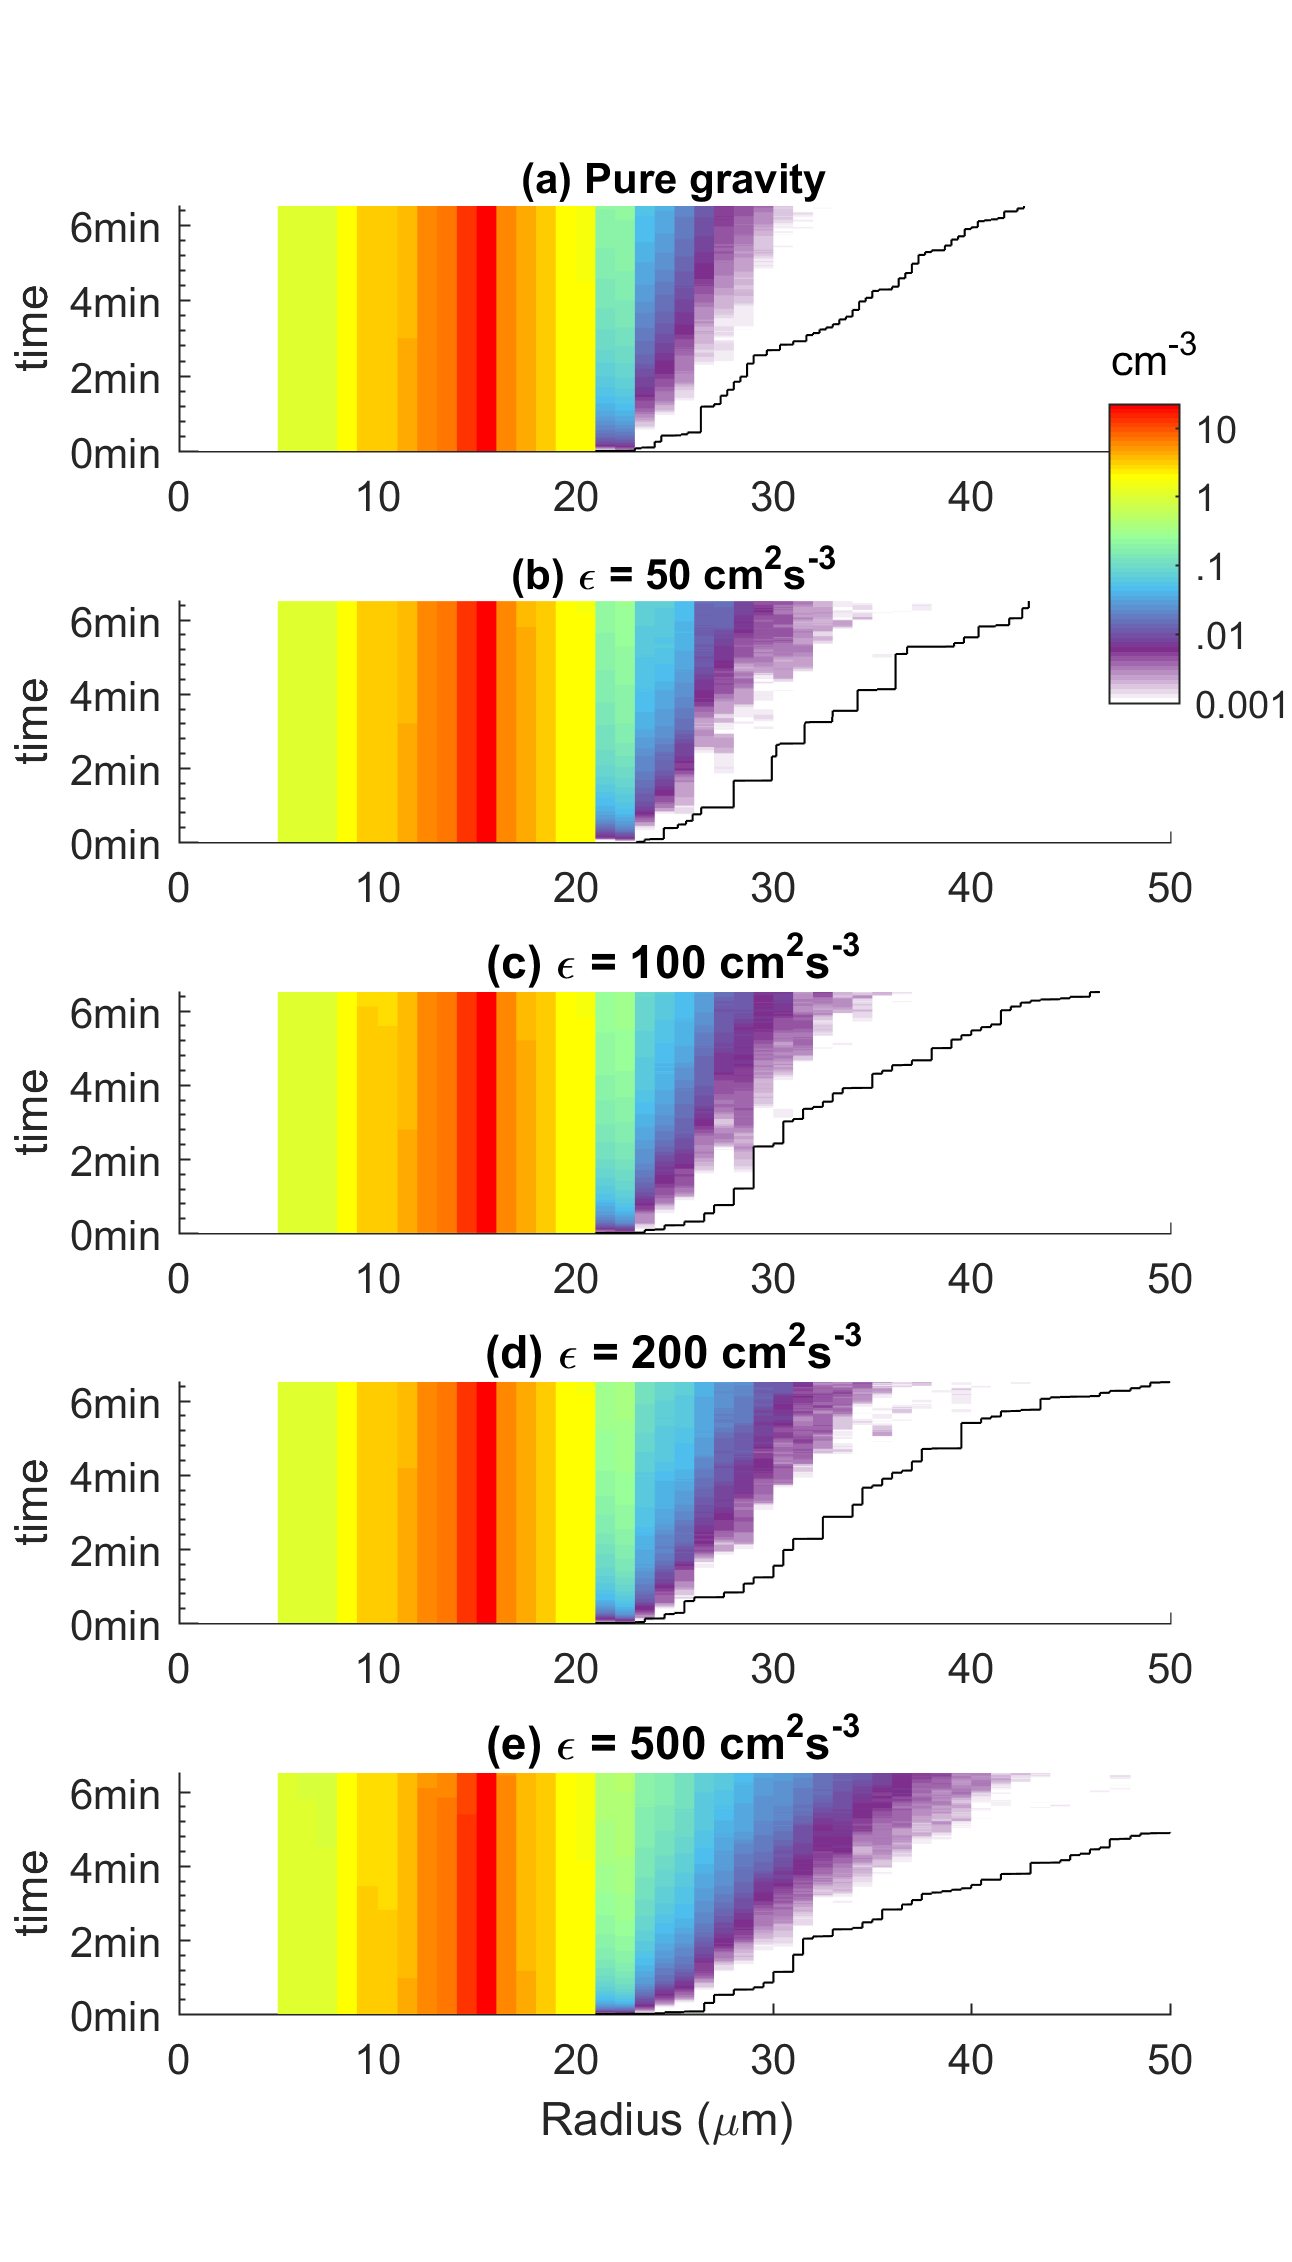
\includegraphics[width=0.5\textwidth]{Figures/Chap3/timeDSD.png}
\caption{: Evolution of droplet size spectra from the same four simulations as described in Fig \ref{fig:DSD}. The color demarcates different number concentrations of each droplet-size bin, with white mapping the concentration below 0.001 $cm^{-3}$. The black curve indicates the size of the largest droplet that occurs in the simulation.} \label{fig:timeDSD}
\end{figure}


To evaluate the collision contribution to the DSD evolution from different r-ratios, we calculate the average collision frequency during the simulation for droplet pairs in various r-ratio bins (Fig. \ref{fig:freq}). As turbulence intensifies, a considerably higher collision frequency is observed from all size groups. Particularly, the largest increment comes from similar-sized collisions. At the pure gravity case, most collisions are from $r_1/r_2\in(0.6,0.8)$. When turbulence gets stronger, the collision frequency distribution becomes heavily skewed. In the simulation of dissipation rate 500 $cm^2s^{-3}$ the number of collisions with $r/r_2>0.9$ increases by more than a factor of 10 compared to the gravitational case, while the enhancement factor of collisions from $r_1/r_2\in(0.6,0.8)$ is smaller than 4. Table \ref{tab:collision} lists the contribution of collisions (probability density function) from different r-ratio ranges. In turbulent cases, similar-sized collisions ($r_1/r_2 > 0.8$) alone account for nearly a quarter of the total collisions. In contrast, only 9.36\% of the collisions are from similar-sized collisions in the gravitational case. In other words, the enhanced broadening by turbulence is largely coming from similar-sized droplet collisions, and even a weak turbulent environment can boost those collisions. However it should be noted that the superposition method does not treat the lubrication effect adequately \citep{Rosa2011,Wang2005a}, and thus the likely overestimation of collision efficiency may lead to faster droplet growth in both the pure-gravity case and the turbulent case.
 

\begin{figure}[ht]
\centering
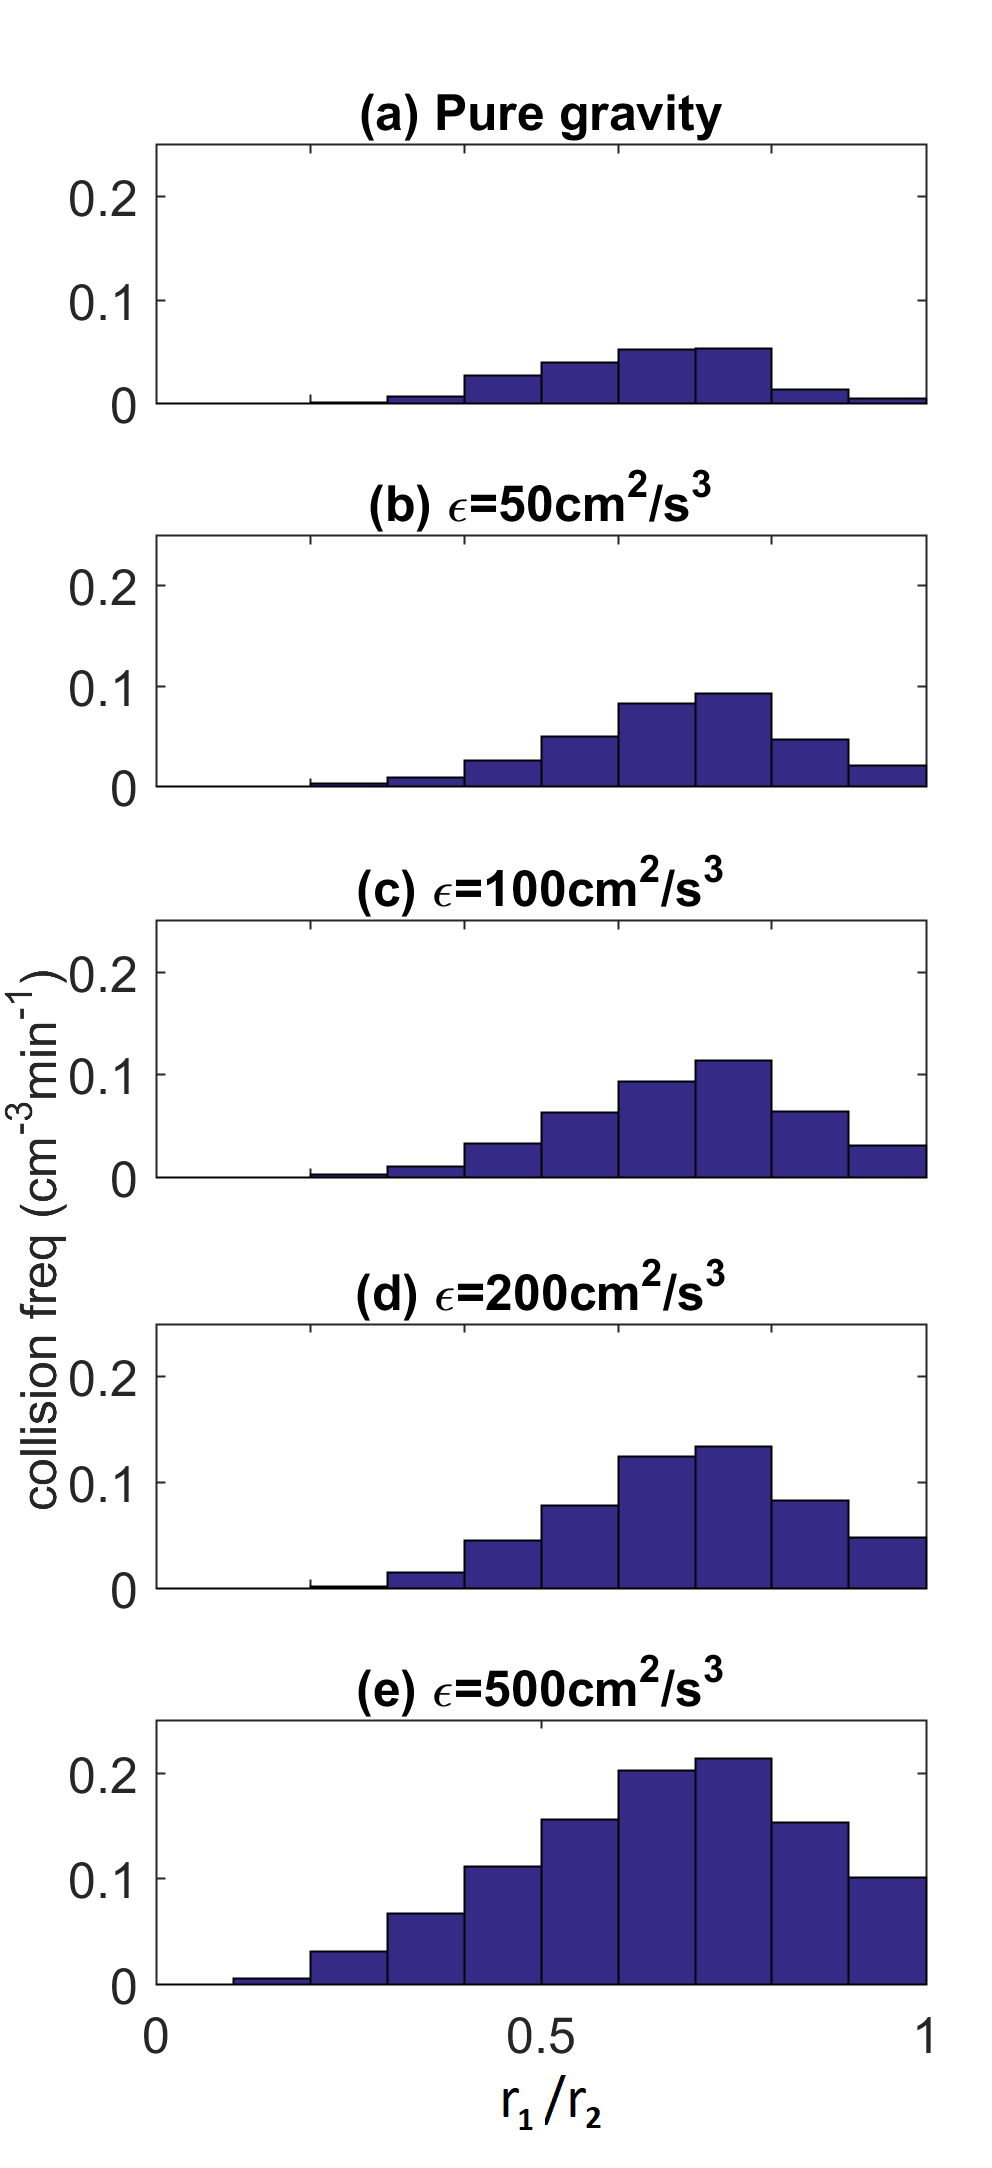
\includegraphics[width=0.4\textwidth]{Figures/Chap3/freq.png}
\caption{Frequency distribution of collisions from different droplet size groups (i.e., different r-ratios) from the four different turbulence environments. The collision frequency is defined as the average number of collisions occurring in each r-ratio bin in unit time ($min ^{-1}$) and in unit volume ($cm^{-3}$) during the entire 6.5 min simulation. The r-ratio is equally divided into ten bins with 0.1 of width for each bin.} \label{fig:freq}
\end{figure}

\begin{table}[ht]
\begin{center}
\caption{contributions (\%) of collisions from different r-ratio ranges in four turbulent cases during 6.5 min simulation.\strut}\label{tab:collision}
\begin{tabular}{c|ccccc}
\hline\hline
\backslashbox{$r_1/r_2$}{$\epsilon$ ($cm^2s^{-3}$)} & 0 & 50 & 100 & 200 & 500 \\
\hline
(0,0.3] & 0.65\% & 1.09\% & 0.53\% & 0.38\% & 3.54\%\\
(0.3,0.8] & 89.99\% & 78.38\% & 76.24\% & 74.89\% & 72.08\% \\
 (0.8,1] & 9.36\% & 20.53\% & 23.23\% & 24.72\% & 24.38\% \\
  \hline
\end{tabular}
\end{center}
\end{table}


\section{Summary and outlook} \label{sec:ch3_conclusion}

The purpose of this study is to investigate and quantify the turbulence enhancement of collision efficiency as part of our continued exploration of turbulence effects on droplet growth. DNS simulations are performed to obtain turbulent collision statistics from 28 droplet-size combinations. LWC is kept at the order of typical adiabatic values to ensure that the hydrodynamic interaction between droplets possibly affected by droplet separation distance (far-field effect) well represents the typical situation in cumulus clouds. Sensitivity tests show little dependency of collision efficiency on LWC values used in this study, suggesting that far-field effects of the disturbance flow have a secondary influence. 

Five dissipation rates spanning a typical range in cumulus clouds ($\epsilon = 20-500$ $cm^2s^{-3}$) are considered, and the pure gravitational case is conducted as a control run. Overall, the turbulence effect of collision efficiency is strongly influenced by the r-ratio. In particular, similar-sized collisions experience the most pronounced enhancement. Previous studies found that turbulent enhancement of the geometric collision kernel is also strongest at similar-sized collisions (r-ratio $\rightarrow$ 1). The joint turbulence effects consolidate a significant increase of the collision kernel between similar-sized droplets. This implies that turbulence can be an effective mechanism to broaden the narrow droplet size distribution resulting from the condensational-growth stage. In addition, we find that for the droplet sizes considered, the enhancement shows little dependency on the size of collector droplet if the r-ratio is fixed. This may simplify the future parameterization as only one size parameter (r-ratio) needs to be considered for those droplet sizes. 


To further illustrate the DSD broadening process and monitor the appearance of large droplets in the early rain formation stage, this study conducts the first direct simulation of the droplet growth by collision-coalescence in the disturbed turbulence flow. The pure-gravity case along with four turbulence intensities ($\epsilon = 50-500$ $cm^2s^{-3}$) are examined with the same initial DSD adopted from aircraft observations of cumulus clouds. While DSD broadening is observed in all simulations, the broadest spectrum occurs in our strongest turbulence. In comparison to the gravitational case, where the DSD stays narrow and droplets hardly exceed 30 $\mu$m throughout the simulation, droplets larger than 35 $\mu$m are seen in all turbulence simulations. In the meantime, similar-sized collisions account for more than 20\% in all turbulent cases ($\epsilon = 50-500$ $cm^2s^{-3}$), compared to less than 10\% in the pure-gravity case. This shows that even weak turbulence is favorable for a significant speed-up of the collision-coalescence process, which reinforces our argument that turbulence broadens the DSD greatly from enhanced similar-sized droplet collisions. 

However, it should be noted that thermodynamic processes, such as CCN activation and droplet diffusional growth, are not included in the model. As collision rate depends highly on the r-ratio, droplet condensational growth, which narrows the size spectra, will push the droplet r-ratio towards unity. We expect that condensation processes may dynamically alter the collision efficiency and the collision kernel. Future work that simultaneously incorporates both processes is required to explore the feedback of droplet condensational growth on the droplet collision rate in a turbulent environment and improve our understanding of turbulence effects on cumulus cloud development and rain initiation.

\acknowledgments
We would like to thank the three anonymous reviewers for their valuable comments. We also thank Mr. Christopher Gagnon for his contribution to analyzing the collision efficiency data. Computations were made on the supercomputer Mammouth II parall\`{e}le from Universit\'{e} de Sherbrooke and supercomputer Guillimin from McGill University, managed by Calcul Qu\'{e}bec and Compute Canada. The operation of this supercomputer is funded by the Canada Foundation for Innovation (CFI), the minist\`{e}re de l'\'{E}conomie, de la science et de l'innovation du  Qu\'{e}bec(MESI) and the Fonds de recherche du Qu\'{e}bec - Nature et technologies (FRQ-NT).


\cleardoublepage 


%========== Chapter 4 
\typeout{}
\resetdatestamp

\chapter{Turbulence impact on warm-rain initiation}\label{sec:ch4}

In previous chapters, we have conducted numerical experiments that only consider the droplet collisional process. In this chapter, we resolve the microscopic and macroscopic thermodynamic processes by including water vapor and temperature fields in the model so that droplets grow by condensation and collision-coalescence simultaneously. The focus of this chapter is to investigate the impact of turbulence on the full set of droplet growth processes and the potential importance of the interaction between condensational and collisional processes. The goal is to answer the following questions:  1) What is the contribution of the droplet condensational process in raindrop formation and how does it interact with the collisional process in a turbulent environment? 2) How does turbulence modulate such interactions? 3) How does the droplet size distribution evolve and how fast do raindrops form under different turbulent conditions? 

This chapter consists of a paper published in Atmospheric Chemistry and Physics: Sisi Chen, M.K. Yau, Peter Bartello, and Lulin Xue: Bridging the condensation-collision size gap: a direct numerical simulation of continuous droplet growth in turbulent cloud, \url{https://doi.org/10.5194/acp-2018-28}
\newpage

\section*{\centering Bridging the condensation-collision size gap: a direct numerical simulation of continuous droplet growth in turbulent cloud}
\begin{center}
\author{Sisi Chen, M. K. Yau, Peter Bartello \\ \textit{Department of Atmospheric and Oceanic Sciences, McGill University, Montr\'{e}al, Qu\'{e}bec, Canada}\\}
\author{Lulin Xue \\ \textit{National Center for Atmospheric Research, Boulder, Colorado, USA}}

\end{center}

\section*{\centering{Abstract}}
In most previous direct numerical simulation (DNS) studies on droplet growth in turbulence, condensational growth and collisional growth were treated separately. Studies in recent decades have postulated that small-scale turbulence may accelerate droplet collisions when droplets are still small when condensational growth is effective. This implies that both processes should be considered simultaneously to unveil the full history of droplet growth and rain formation. This paper introduces the first DNS approach to explicitly study the continuous droplet growth by condensation and collisions inside an adiabatic ascending cloud parcel. Results from the condensation-only, collision-only, and condensation-collision experiments are compared to examine the contribution to the broaden	ing of droplet size distribution by the individual process and by the combined processes. Simulations of different turbulent intensities are conducted to investigate the impact of turbulence on each process and on the condensation-induced collisions. The results show that the condensational process promotes the collisions in a turbulent environment and reduces the collisions when in still air, indicating a positive impact of condensation on turbulent collisions. This work suggests the necessity to include both processes simultaneously when studying droplet-turbulence interaction to quantify the turbulence effect on the evolution of cloud droplet spectrum and rain formation.

\section{Introduction} \label{sec:ch4_intro}

Theoretical studies indicate that for droplets in the size range of 15-30$\mu m$ in radius, referred to as the condensation-collision size gap, neither condensational growth nor collisional growth is effective \citep{Pruppacher1997} in producing precipitation. Classical parcel models generally yielded very narrow droplet size distributions (DSDs) and take a rather long time to form rain \citep{Jonas1996}. In nature, wide DSDs and large droplets are frequently observed in cumulus and even statocumulus clouds \citep[e.g.,][]{BC2001,Pawlowska2006,Prabha2012}. This size gap problem represents a longstanding challenge in the ongoing quest to understand the warm-rain initiation process. In the literature, various mechanisms have been proposed to accelerate rain development, such as small-scale turbulence \citep{Vaillancourt2000}, the presence of giant aerosols \citep{johnson1982,blyth2003,Jensen2017}, entrainment of unsaturated air \citep{baker1980,lasher2005,cooper2013} and large-eddy hopping \citep{cooper1989,grabowski2017}. This study focuses on the effect of small-scale turbulence containing eddies in the inertial and dissipation range with length-scales $\ll$ 10 m as shown in Fig. 1 of \citet{Grabowski2013}, which can be resolved by the technique of direct numerical simulation (DNS). 

Several mechanisms related to turbulence have been proposed to explain the fast growth of droplets in the condensation-collision size gap \citep{Devenish2012,Grabowski2013}. As a result of the response of droplet inertia to turbulent eddies of different scales, turbulent flow creates two effects: the non-uniform distribution of cloud droplets (clustering effect) and the increase in the relative velocities between droplets (transport effect). A number of DNS studies have reported that the geometric collision rate of droplets increases as turbulence intensifies \citep{Franklin2005, Ayala2008a,Onishi2016}. Concomitantly, turbulence modifies the response of a droplet to the local disturbance flow induced by other droplets through hydrodynamic interactions to increase the collision efficiency \citep{Wang2008, Onishi2013, Chen2018}. In particular, \citet{Chen2018} demonstrated that the turbulence enhancement of collisions became most significant among droplet pairs of similar sizes, suggesting that turbulence may efficiently broaden the narrow DSD generated from condensational growth.

Moreover, it has also been argued that the supersaturation perturbation field can arise from the fluctuation of temperature and water vapor in turbulence and the differential local water vapor consumption \citep{Srivastava1989} which is enhanced by droplet clustering. This may lead to a distinct growth history by condensation for each droplet as it is transported in a turbulent flow \citep{Lanotte2009}. However, several DNS studies found that small-scale turbulence can only create small, if not insignificant, drop size broadening through condensation \citep{Vaillancourt2002,Lanotte2009, Sardina2015}. The reason is that the average time that droplets are exposed to supersaturation perturbations shortens as the turbulence intensifies and as droplets grow larger and begin to sediment \citep{Vaillancourt2002}. \citet{Lanotte2009} reported a wider size distribution when the Reynolds number of the flow, which is calculated based on the computational domain size, increased from 40 to 185 and proposed a simple scaling to extrapolate the DNS result to the typical size of a cloud adiabatic core (approximately 100 m wide or Reynolds number $\approx 5000$). However, caution should be exercised in applying this scaling as DNS is not able to capture the spatiotemporal complexity of the turbulence at scales larger than the size of the domain. \citet{Sardina2015} also used a similar model as \citet{Lanotte2009} but extended the simulation time to 20 minutes to be comparable to the formation time of rain revealed in real observations. They found that the variance of the droplet size distribution was mainly determined by the large-scale flow, i.e., the large-hopping effect suggested by \citet{Grabowski2013} and studied by \citet{grabowski2017}. Nevertheless, it should be noted that their conclusion was based on the simplified assumption that both the mean updraft speed and the mean supersaturation were zero. On the other hand, the DNS model of \citet{Gotoh2016} considered a time-dependent and buoyancy-driven mean vertical motion calculated from a given environmental sounding. In their study of the effect of turbulence and entrainment on the evolution of cloud droplets, it was found that the thermodynamic fluctuations caused by turbulent advection prevented the buildup of the buoyancy force, leading to an even slower evolution of the mean droplet size and the vertical velocity as compared to those predicted by a parcel model. 

A common limitation shared by most, if not all, previous DNS studies is that, the condensation process and collision-coalescence process were studied separately. This assumption may be justifiable in a parcel model due to the non-overlapping droplet-size regimes of the two growth processes in still-air. However, this assumption is questionable in DNS studies, which reveal substantial turbulent enhancement of collisions among droplets in the condensation-collision size gap. As there is an absence of DNS work on continuous droplet growth incorporating both processes, it is the goal of this study to unveil the full history of droplet growth and DSD broadening by condensational and collisional growth in a turbulent, supersaturated environment undergoing an adiabatic ascent. 

The purpose of this study is: 1) to introduce the first DNS approach to explicitly resolve the continuous droplet growth by condensation and collision in shallow, turbulent clouds, and 2) to answer the following two questions: “how does the droplet collisional process interact with the droplet condensational growth process?” and “what is the role of turbulence in this interaction? “

Our approach is to incorporate the droplet hydrodynamic collision and condensation processes into a single DNS modeling framework. Arguably, this model provides a first direct approach to bridge the condensation-collision gap that has puzzled the cloud physics community for decades. The paper is organized as follows. In Sect. \ref{sec:ch4_method} we describe the sets of equations adopted from \citet{Vaillancourt2001} and Chapter \ref{sec:ch3} \citep{Chen2018} and the accompanying modification. The simulated results from three sets of experiments (condensation-only, collision-only, condensation-collision) in various turbulent environments are given in Sect. \ref{sec:ch4_result}, to be followed by a conclusion and remarks on the limitation of this study in Sect. \ref{sec:ch4_conclusion}.

\section{Model description and experimental setup}\label{sec:ch4_method}
This Chapter represents a sequel to Chapter \ref{sec:ch3} as part of our on-going exploration of the evolution of cloud DSD affected by turbulence. The DNS model adopted was originally developed by \citet{Vaillancourt2001} in perhaps one of the earliest DNS approaches to simulate droplet growth in turbulence. \citet{Vaillancourt2001} focused on the impact of turbulence on droplet condensation, and thus collisions were not considered. A number of extensions followed. \citet{Franklin2005} resolved the droplet collisions using an efficient collision detection technique. In Chapter \ref{sec:ch2}, we made changes to allow simulation in larger domain sizes and introduced a new forcing scheme to achieve a statistically steady turbulent dissipation rate. Chapter \ref{sec:ch3} added the local disturbance flow field induced by droplets to obtain accurate turbulent collision efficiencies and droplet collisional growth affected by both the disturbance flow and the turbulence flow. 

In the present study, the model from Chapter \ref{sec:ch3} is further extended to restore the thermodynamical framework of \citet{Vaillancourt2001} to include condensational growth. Specifically, the whole DNS box is regarded as a parcel ascending adiabatically from near the cloud base with a constant mean updraft. Two sets of equations are used to solve for 1) the macroscopic variables that describe the time evolution of the parcel mean state properties and 2) the microscopic variables that describe the turbulent flow, as well as the temperature and the water vapor mixing ratio fluctuation fields. Furthermore, equations pertaining to the thermodynamics are modified to improve the accuracy of droplet condensational growth.

In the presence of the thermodynamic fluctuation fields and the turbulence flow field, droplets grow in two distinct ways simultaneously:

1) Droplets grow by condensation with its growth rate directly proportional to the instantaneous supersaturation (see Eq. (\ref{eq:cond_growth})). When a droplet moves relative to the air, the water vapor field is not spherically symmetric around the droplet surface but is modified depending on the direction of motion (so-called the ventilation effect). This effect becomes important when droplets are greater than 30 $\mu m$ in radius \citep{sedunov1974}. In \citet{Vaillancourt2001}, all droplets were smaller than 20 $\mu m$ and this effect was not considered. However, the present study allows droplets to grow larger and thus the ventilation coefficient is added to the droplet growth equation. Following \citet{Vaillancourt2001}, the curvature term and the solute term are neglected in the equation, and the droplets are treated as pure water drops since all droplets in this study are greater than 5 $\mu m$ \citep{Pruppacher1997}.

2) Simultaneously, droplets grow through the collision-coalescence process. The droplet motion and collisional growth are treated in the same manner as in Chapter \ref{sec:ch3}. Each droplet is tracked in the Lagrangian framework, with its motion determined by gravity and the local fluid drag force (equation (\ref{eqn:dropmotion})). Once two droplets collide, they coalesce to become a bigger entity with its mass equal to the sum of the masses of the collided droplets and its location being the barycenter of the binary system before the collision. The velocity of the coalesced droplet is calculated based on the conservation of momentum. Since we are particularly interested in the condensation-collision size range, i.e., droplets smaller than drizzle drops, defined as drops with a radius equal to larger than 100 $\mu m$, our study only consider radius $r\ll$ 100 $\mu m$. In addition, solving the motion of large drops requires more complex consideration such as induced turbulent wakes and drop deformation which are beyond the scope of this study. Therefore, droplets reaching 100 $\mu m$ are considered as fall-outs and are not allowed to grow further, i.e., they neither interact with other droplets nor affect the local disturbance flows. It should be noted that this assumption bears certain caveats. The Stokes' Law assumption for the disturbance flow becomes less accurate for droplets larger than 50 $\mu m$, because droplets over 50 $\mu m$ (and smaller than 100 $\mu m$) have a particle Reynolds number of order one. However, since the collision efficiency for droplets larger than 50 $\mu m$ is close to unity due to the large Stokes number, it is argued that the impact of the disturbance flow on the collision statistics of those large particles would be secondary. Furthermore, in all the simulations the calculated total number of collisions remains below 10\% of the total number of droplets. Specifically, the number of collisions is within 9\% in strong turbulence and below 3\% in weak turbulence and below 2\% in still air. It follows that the impact of reducing the droplet number concentration due to collisions on the resulting DSD can be assumed small. One alternative post-collision treatment maybe to introduce a new, randomly located droplet into the domain once a collision happens so that the droplet number concentration remains constant. However, the size of droplets that should be introduced remains contentious and needs further justification.
 

The detailed equations are provided as below.

\subsection{Microscopic equations}\label{sec:micro}
The condensational growth rate of an individual droplet with radius $r_i$ is as follow:
\begin{equation}\label{eq:cond_growth}
\frac{dr_i^2}{dt}=2Kf_vS.
\end{equation}

 Here $K^{-1}=\frac{\rho_wR_vT}{e_{sat}(T)D_v}+\frac{L\rho_w}{K_aT}(\frac{L}{R_vT}-1)$, where $e_{sat}$ is the saturated water vapor pressure. $f_v$ refers to the droplet ventilation coefficient. The value of $f_v$ is determined by the empirical formulas from laboratory experiment of \citet{Beard1971}:
\begin{equation}
f_v=1.0+0.108(N_{Sc}^{1/3}Re_p^{1/2})^2,\text{   for  $N_{Sc}^{1/3}Re_p^{1/2}<1.4$},
\end{equation}
\begin{equation}
f_v=0.78+0.308(N_{Sc}^{1/3} Re_p^{1/2} ),\text{  for $51.4>N_{Sc}^{1/3} Re_p^{1/2}\geq 1.4$},
\end{equation}
where $Re_p=\frac{2r_i|\bf{V}|}{\nu}$ is the droplet Reynolds number, $\mathbf{V}$ is the velocity of droplet i. $S$ is the supersaturation in the grid cell where droplet i is located, defined as 
\begin{equation}\label{eq:supersat}
S=\frac{q_v}{q_{vs}}-1,
\end{equation} 
where $q_v$ is the water vapor mixing ratio, with its corresponding saturated value $q_{vs}$ determined by temperature ((2.17)-(2.18) in Rogers and Yau 1989). We assume that all droplets residing in the same grid cell are exposed to the same supersaturation environment. The scaler fields of $q_v$ and temperature $T$ can be decomposed into the parcel mean state and the perturbation state. The parcel mean state is calculated via the macroscopic set of equations shown in Sect. \ref{sec:macro} and the perturbations are calculated as follows:
\begin{equation}\label{eq:temp}
\frac{\partial{T^\prime}}{\partial{t}} = -\mathbf{\nabla}\cdot(\mathbf{U}T^\prime)-W^\prime\Gamma_d + \frac{L}{C_p}C_d^\prime+D_t\nabla^2T^\prime,
\end{equation}
\begin{equation}\label{eq:qv}
\frac{\partial{q_v^\prime}}{\partial{t}} = -\mathbf{\nabla}\cdot(\mathbf{U}q_v^\prime)-C_d^\prime+D_v\nabla^2q_v^\prime,
\end{equation}
where $W^\prime$ is the vertical perturbation velocity. $C_d^\prime = C_d - C_{dM}$ is the differential condensation rate between the grid cell and the whole parcel. Given (\ref{eq:cond_growth}), the condensation rate inside the grid cell can be simplified as:
\begin{equation} \label{eq:C_d}
C_d= \frac{1}{m_a}\sum^n_i{\frac{4}{3}\pi\rho_w\frac{dr_i^3}{dt}}=\frac{4}{m_a}\pi\rho_wKf_v\sum^n_i{r_iS}.
\end{equation}

The turbulent velocity field $\mathbf{U}$ is governed by the incompressible Navier-Stokes equations:
\begin{equation} \label{eq:NSeq}
\frac{\partial \mathbf{U}}{\partial t}+(\mathbf{U}\cdot\nabla) \mathbf{U} = -\frac{1}{\rho_a}\nabla P+\nu \nabla^2\mathbf{U}+\mathbf{F},
\end{equation}
\begin{equation} \label{eq:incomp}
\nabla\cdot\mathbf{U}=0,
\end{equation}
where P is the perturbation pressure deviation from the hydrostatic pressure $P_M$. The pressure term can be dropped when the equations are solved in vorticity form. $\mathbf{F}$ is the external forcing. We used the forcing method of \citet{Chen2016} to maintain the turbulence. The droplet motion is governed by fluid drag force and gravity:

\begin{equation}
\frac{d\mathbf{V}(t)}{dt}=\frac{\mathbf{V}(t)-\tilde{\mathbf{U}}(\mathbf{X}(t),t)}{\tau_p}+\mathbf{g}, \label{eqn:drop}
\end{equation}
$\tau_p$ denotes the droplet response time. For $r<40 \mu m$, Stokes drag force is applied and $\tau_p=(\frac{2\rho_w}{9\nu\rho_a})r^2$. Droplet terminal velocity can be obtained using $V_T=g\tau_p$. For $r\geq 40 \mu m$, the terminal velocity derived from the experimental data is applied to those big droplets: $V_T=k_2r$, here $k_2=8 \times 10^3s^{-1}$ \citep[p.126]{Rogers1989}. $\tilde{\mathbf{U}}$ is the flow velocity at the droplet center, contributed by the turbulent flow field $\mathbf{U}$ and the disturbance flow $\mathbf{U_{dist}}$ caused by neighboring droplets \citep{Chen2018}. The superposition method by \citet{Wang2005b} is used to calculate the disturbance flow.

 
\subsection{Macroscopic equations}\label{sec:macro}
The time evolution of the parcel-mean temperature $T_M$, water vapor mixing ratio $q_{vM}$, pressure $P_M$, density $\rho_{aM}$ are described as below. All variables of parcel mean are denoted with a subscript M.
\begin{equation}
\frac{dT_M}{dt}=-W_M\Gamma_d+\frac{L}{C_p}C_dM
\end{equation}
\begin{equation}
\frac{dq_{vM}}{dt}=-C_{dM}
\end{equation}
\begin{equation}
C_{dM}=\frac{1}{M_a} \sum^N_i{\frac{d}{dt}(\frac{4}{3}\pi\rho_wr_i^3)}=\frac{4}{M_a}\pi\rho_wKf_v\sum^N_i{r_iS},
\end{equation}
\begin{equation}
\frac{dP_M}{dt}=-\rho_{aM}gW_M
\end{equation}
\begin{equation}
\rho_{aM}=\frac{P_M}{R_aT_M}
\end{equation}

The total fields of T and $q_v$ are calculated by adding the macroscopic variables and the perturbation variables. 
 
\subsection{Experimental setup}

Three sets of experiments are conducted to evaluate the DSD broadening due to the turbulence effect on different droplet growth processes: 1) droplet growth by condensation only (referred to as the condensation-only experiment), 2) droplet growth by collision-coalescence only (referred to as the collision-only experiment), and 3) droplet growth by condensation and collision-coalescence together (referred to as the condensation-collision experiment), respectively. All experiments use the same initial DSD shape adopted from an aircraft measurement in non-precipitating cumulus clouds \citep{Raga1990}. The initial droplet number concentration is set as 80 $cm^{-3}$ and a constant updraft of 2.5 $ms^{-1}$ is used to represent the condition of pristine maritime cumulus clouds. 

For each set of experiments (except for the condensation-only experiment), three flow configurations are considered: purely-gravitational case (i.e., still air), a weak turbulence case (with eddy dissipation rate $\epsilon= $ 50 $cm^2 s^{-3}$), and a strong turbulence case (with $\epsilon=$ 500 $cm^2 s^{-3}$). The domain size of each simulation is about 10 cm in each direction, with grid space $\approx 0.1$ cm determined by the dissipation rate as explained in \citet{Chen2016}. It is recognized that droplet condensation in still-air leads to a narrow DSD and DSD broadening by condensation impacted by small-scale turbulence is insignificant. Therefore, during the condensation-only experiment, only the strong turbulence simulation is performed to serve as an upper bound of the DSD broadening among the three flow conditions. As a result, seven simulations are performed. Each simulation lasts 6.5 minutes of real-time, which is the approximate duration for the whole parcel to ascend from cloud base to 1000 m above the base, representative of a typical cumulus development. 

\section{Results and discussion}\label{sec:ch4_result}

We first compare the results from the three experiments to scrutinize the contributions of the different droplet growth processes under the effect of turbulence. Figure \ref{fig01} shows the DSDs at the end of each experiment in strong turbulence condition. As a reference, the initial DSD is displayed with a gray area. It should be noted that droplet number concentrations below 0.001 $cm^{-3}$ will be treated as statistical uncertainty throughout the discussion, since they correspond to less than 2-4 droplets in the domain. Consistent with past findings, the turbulence effect on droplet condensational growth is small. The condensation-only process produces the narrowest size distribution among the three experiments and droplets grow no larger than 20 $\mu m$ at the end of the simulation. On the other hand, in both the collision-only experiment (blue curve) and the condensation-collision experiment (yellow curve), a substantial number of large droplets are found. Furthermore, compared to the collision-only simulation, the condensation-collision experiment generates more large droplets and substantially larger droplets. The largest $r$ reaches 100 $\mu m$ at the end of the simulation compared to less than 65 $\mu m$ in the collision-only case. Meanwhile, the number concentration of $r > 30 \mu m$ droplets in the condensation-collision case increases by a factor of 2.3 (0.35 $cm^{-3}$ compared to 0.15 $cm^{-3}$ in the collision-only case). 

\begin{figure}[ht]
\centering
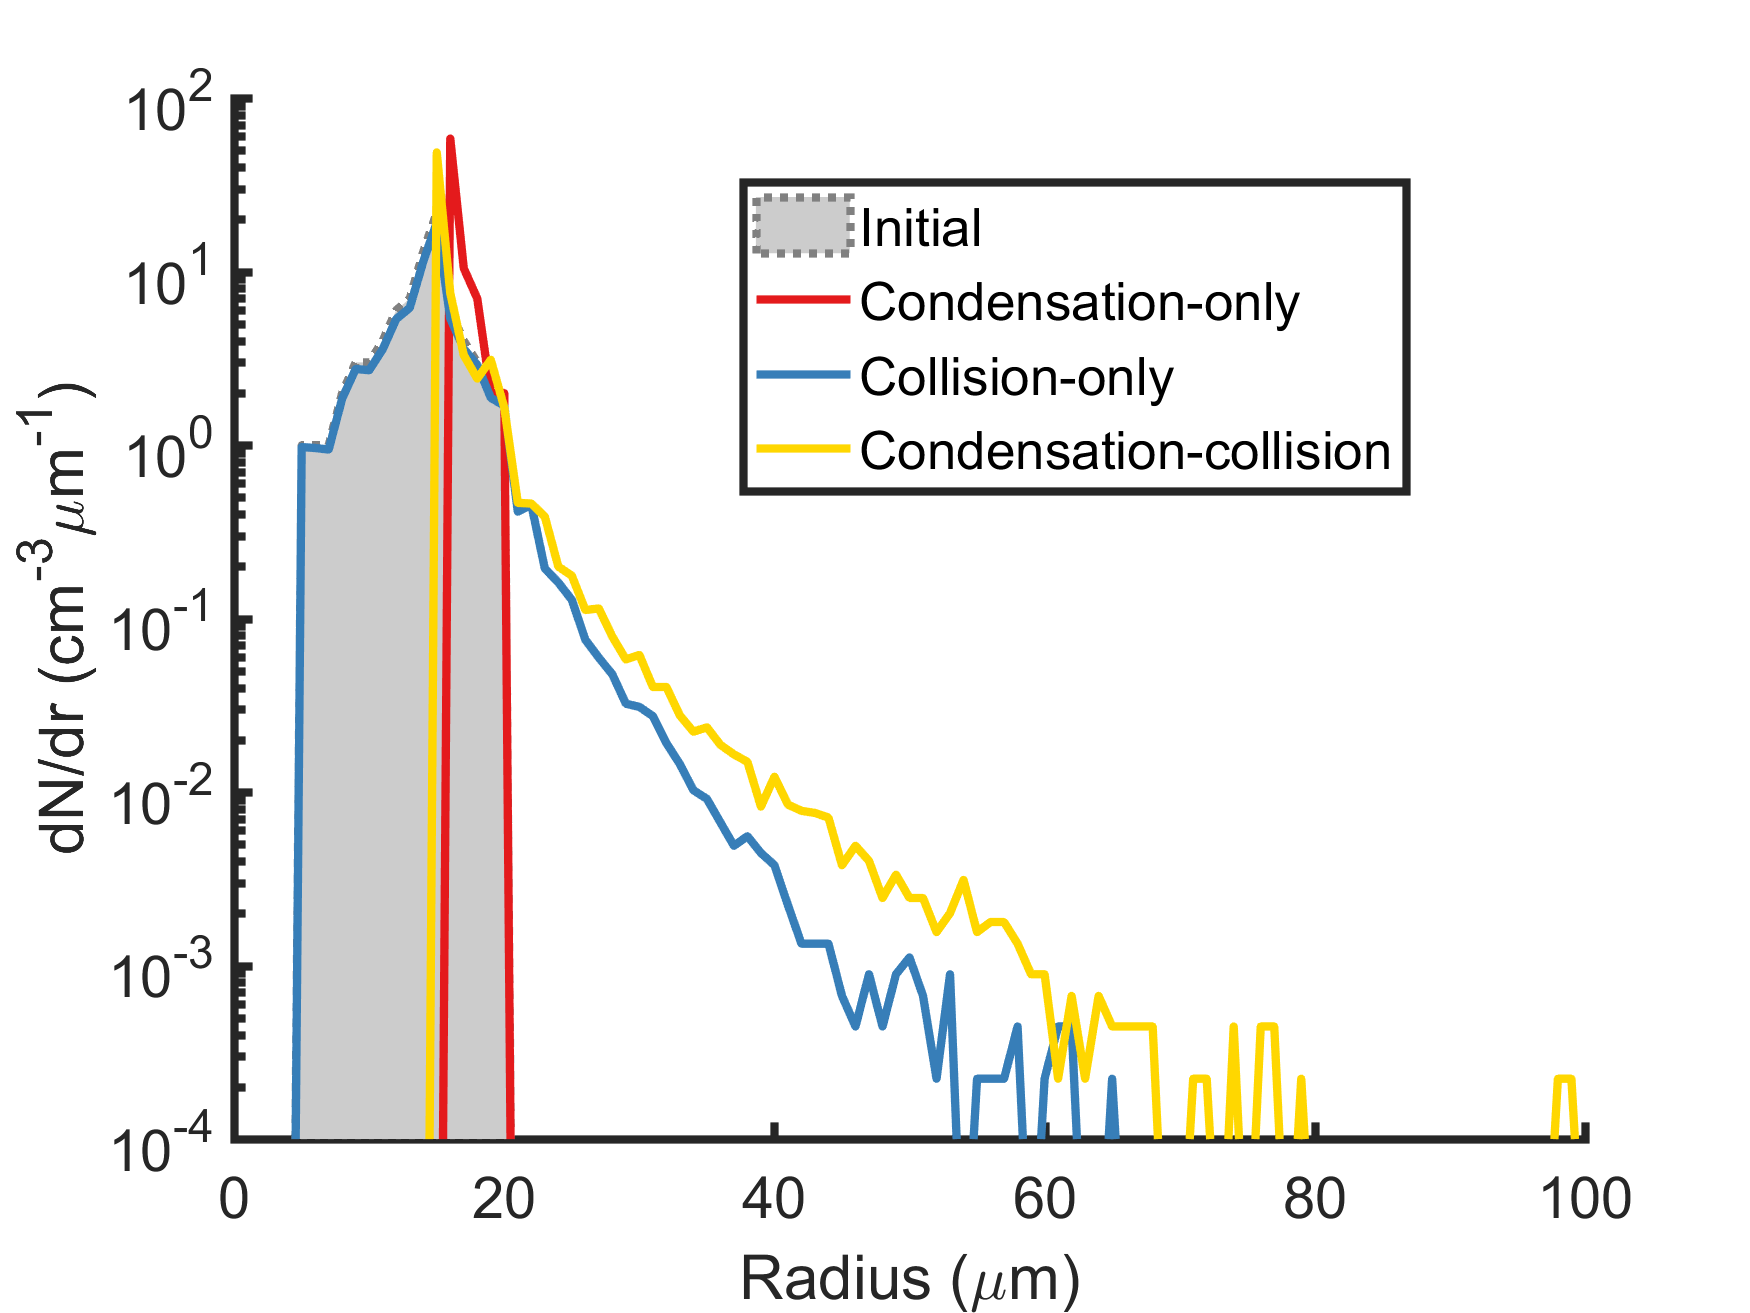
\includegraphics[width=0.8\textwidth]{Figures/Chap4/DSD_end.png}
\caption{Droplet size distributions at the 6.5th minute for the condensation-only case (red), collision only case (blue) and condensation-collision case (yellow). Dissipation rate is 500 $cm^2 s^{-3}$ for all cases with the initial size distribution shown as a dashed grey line. Droplet number concentrations below 0.001 $cm^{-3}$ are treated as statistical uncertainty since they correspond to less than 2-4 droplets in the domain.}\label{fig01}
\end{figure}

To examine whether this enhanced broadening due to the inclusion of the condenational process depends on the flow, detailed comparisons between the collision-only and the condensation-collision experiments are made under three flow conditions: purely-gravitational, weak turbulence, and strong turbulence. Figure \ref{fig02} demonstrates the time evolution of DSD in the two sets of experiments under the three different flows. It is found that:

1) In the purely-gravitational case (Figs. \ref{fig02}(a) and \ref{fig02}(b)), despite the condensation-collision experiment producing larger maximum droplets at the end of the simulation relative to the collision-only experiment (black outline in Fig. \ref{fig02}), the number concentration of large droplets is still negligible (as $r>$ 35 $\mu m$ droplets stay below 0.001 $cm^{-3}$ as seen from the expansion of the purple edge with time);

2) In the turbulent cases, we find more large droplets and much larger maximum droplet sizes in the domain when condensational growth is considered. With weak turbulence droplets larger than 35 $\mu m$ (over 0.001 $cm^{-3}$) can be seen as early as 3.5 minutes in the condensation-collision experiment, but 6 minutes in the collision-only run. With strong turbulence,  large droplets were found in the 3rd minute in the condensation-collision simulation compared to the 4th minute without condensation. It is evidence that both experiments experience earlier formation of large droplets as turbulence intensifies while the inclusion of condensation further accelerate the droplet growth. This result evinces that an effective condensation-collision broadening mechanism exists that strengthened with increasing turbulence intensity.

\begin{figure}[ht]
\centering
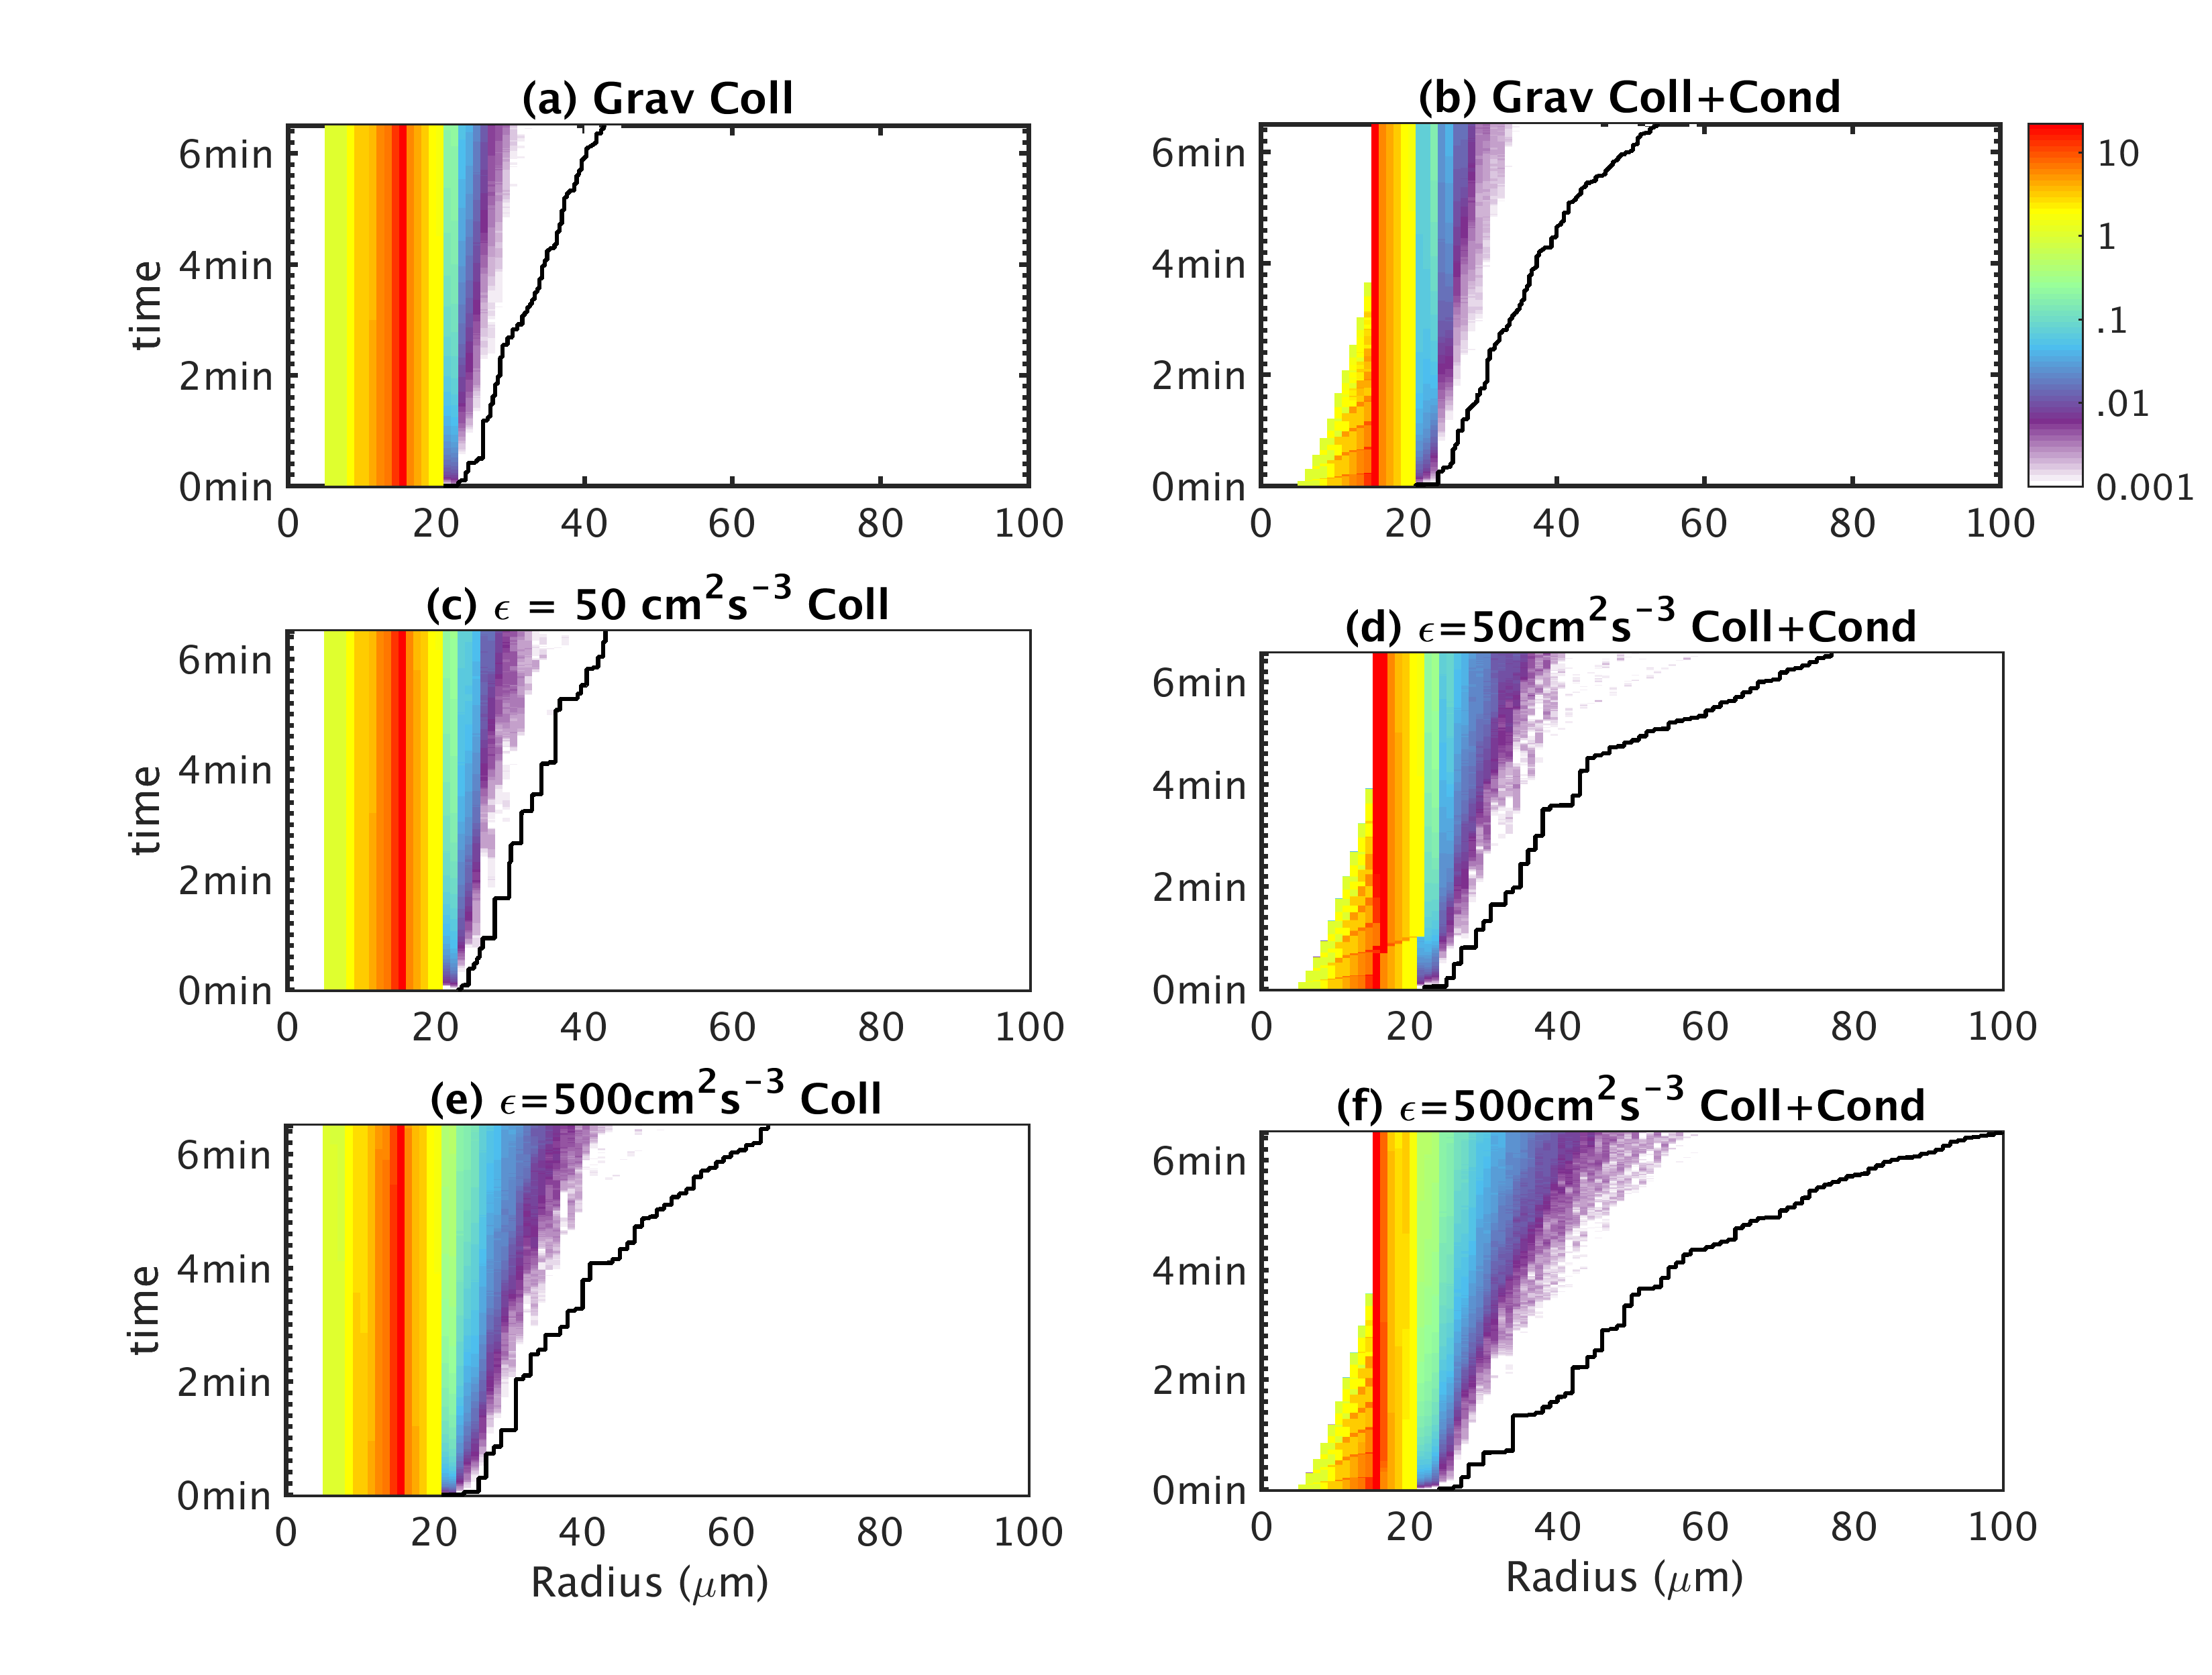
\includegraphics[width=0.8\textwidth]{Figures/Chap4/DSD_evo.png}
\caption{The time evolution of DSD in the collision-only experiments (left column) and the collision-condensation experiments (right column). Results from the purely-gravitational case (first row), weak turbulence ($\epsilon=50$ $cm^2 s^{-3}$, second row), and strong turbulence ($\epsilon=$ 500  $cm^2 s^{-3}$, third row) are demonstrated. The solid black curve indicates the largest droplet of the entire domain. The droplet number concentration ($cm^{-3}$) on each size bin (bin width = 1 $\mu m$) is displayed in color using a logarithmic scaling shown in the color bar. Droplet number concentrations below 0.001 $cm^{-3}$ are treated as statistical uncertainty and thus are given no color in the plot.}\label{fig02}
\end{figure}

A condensation-induced broadening has been found in all three flow conditions, though it seems that it is negligible in the case of still air. This phenomenon can be explained by two main mechanisms:

1)	The condensational growth produces effectively grows droplets of small sizes ($r<$ 10 $\mu m$) to medium size ($10-20$ $\mu m$) due to the fast growth rate of small droplets. This conjecture is supported by the result on the right column of Fig. \ref{fig02} showing that among the three condensational cases, all droplets smaller than 15 $\mu m$ become greater than 15 $\mu m$ within 4 minutes. As bigger droplets have higher collision rates, the average collision rate in the domain is expected to increase progressively as more medium-sized droplets are formed through condensation, and they become more likely to be collected by other droplets.

2)	Condensational growth narrows the DSD and providing a great number of similar-sized droplets (i.e., the radius ratio between the small droplet and large droplet, $r_1/r_2$, is close to unity). \citet{Chen2018} found that turbulence enhancement of collision rate is most significant in similar-sized droplets, and stays relatively weak for $0.2<r_1/r_2<0.8$ (Fig. \ref{fig03} in their paper).  In an environment with similar-sized droplets created by condensation, the turbulence-enhanced collisions are enhanced to accelerate the production of large droplets. 

\begin{figure}[ht]
\centering
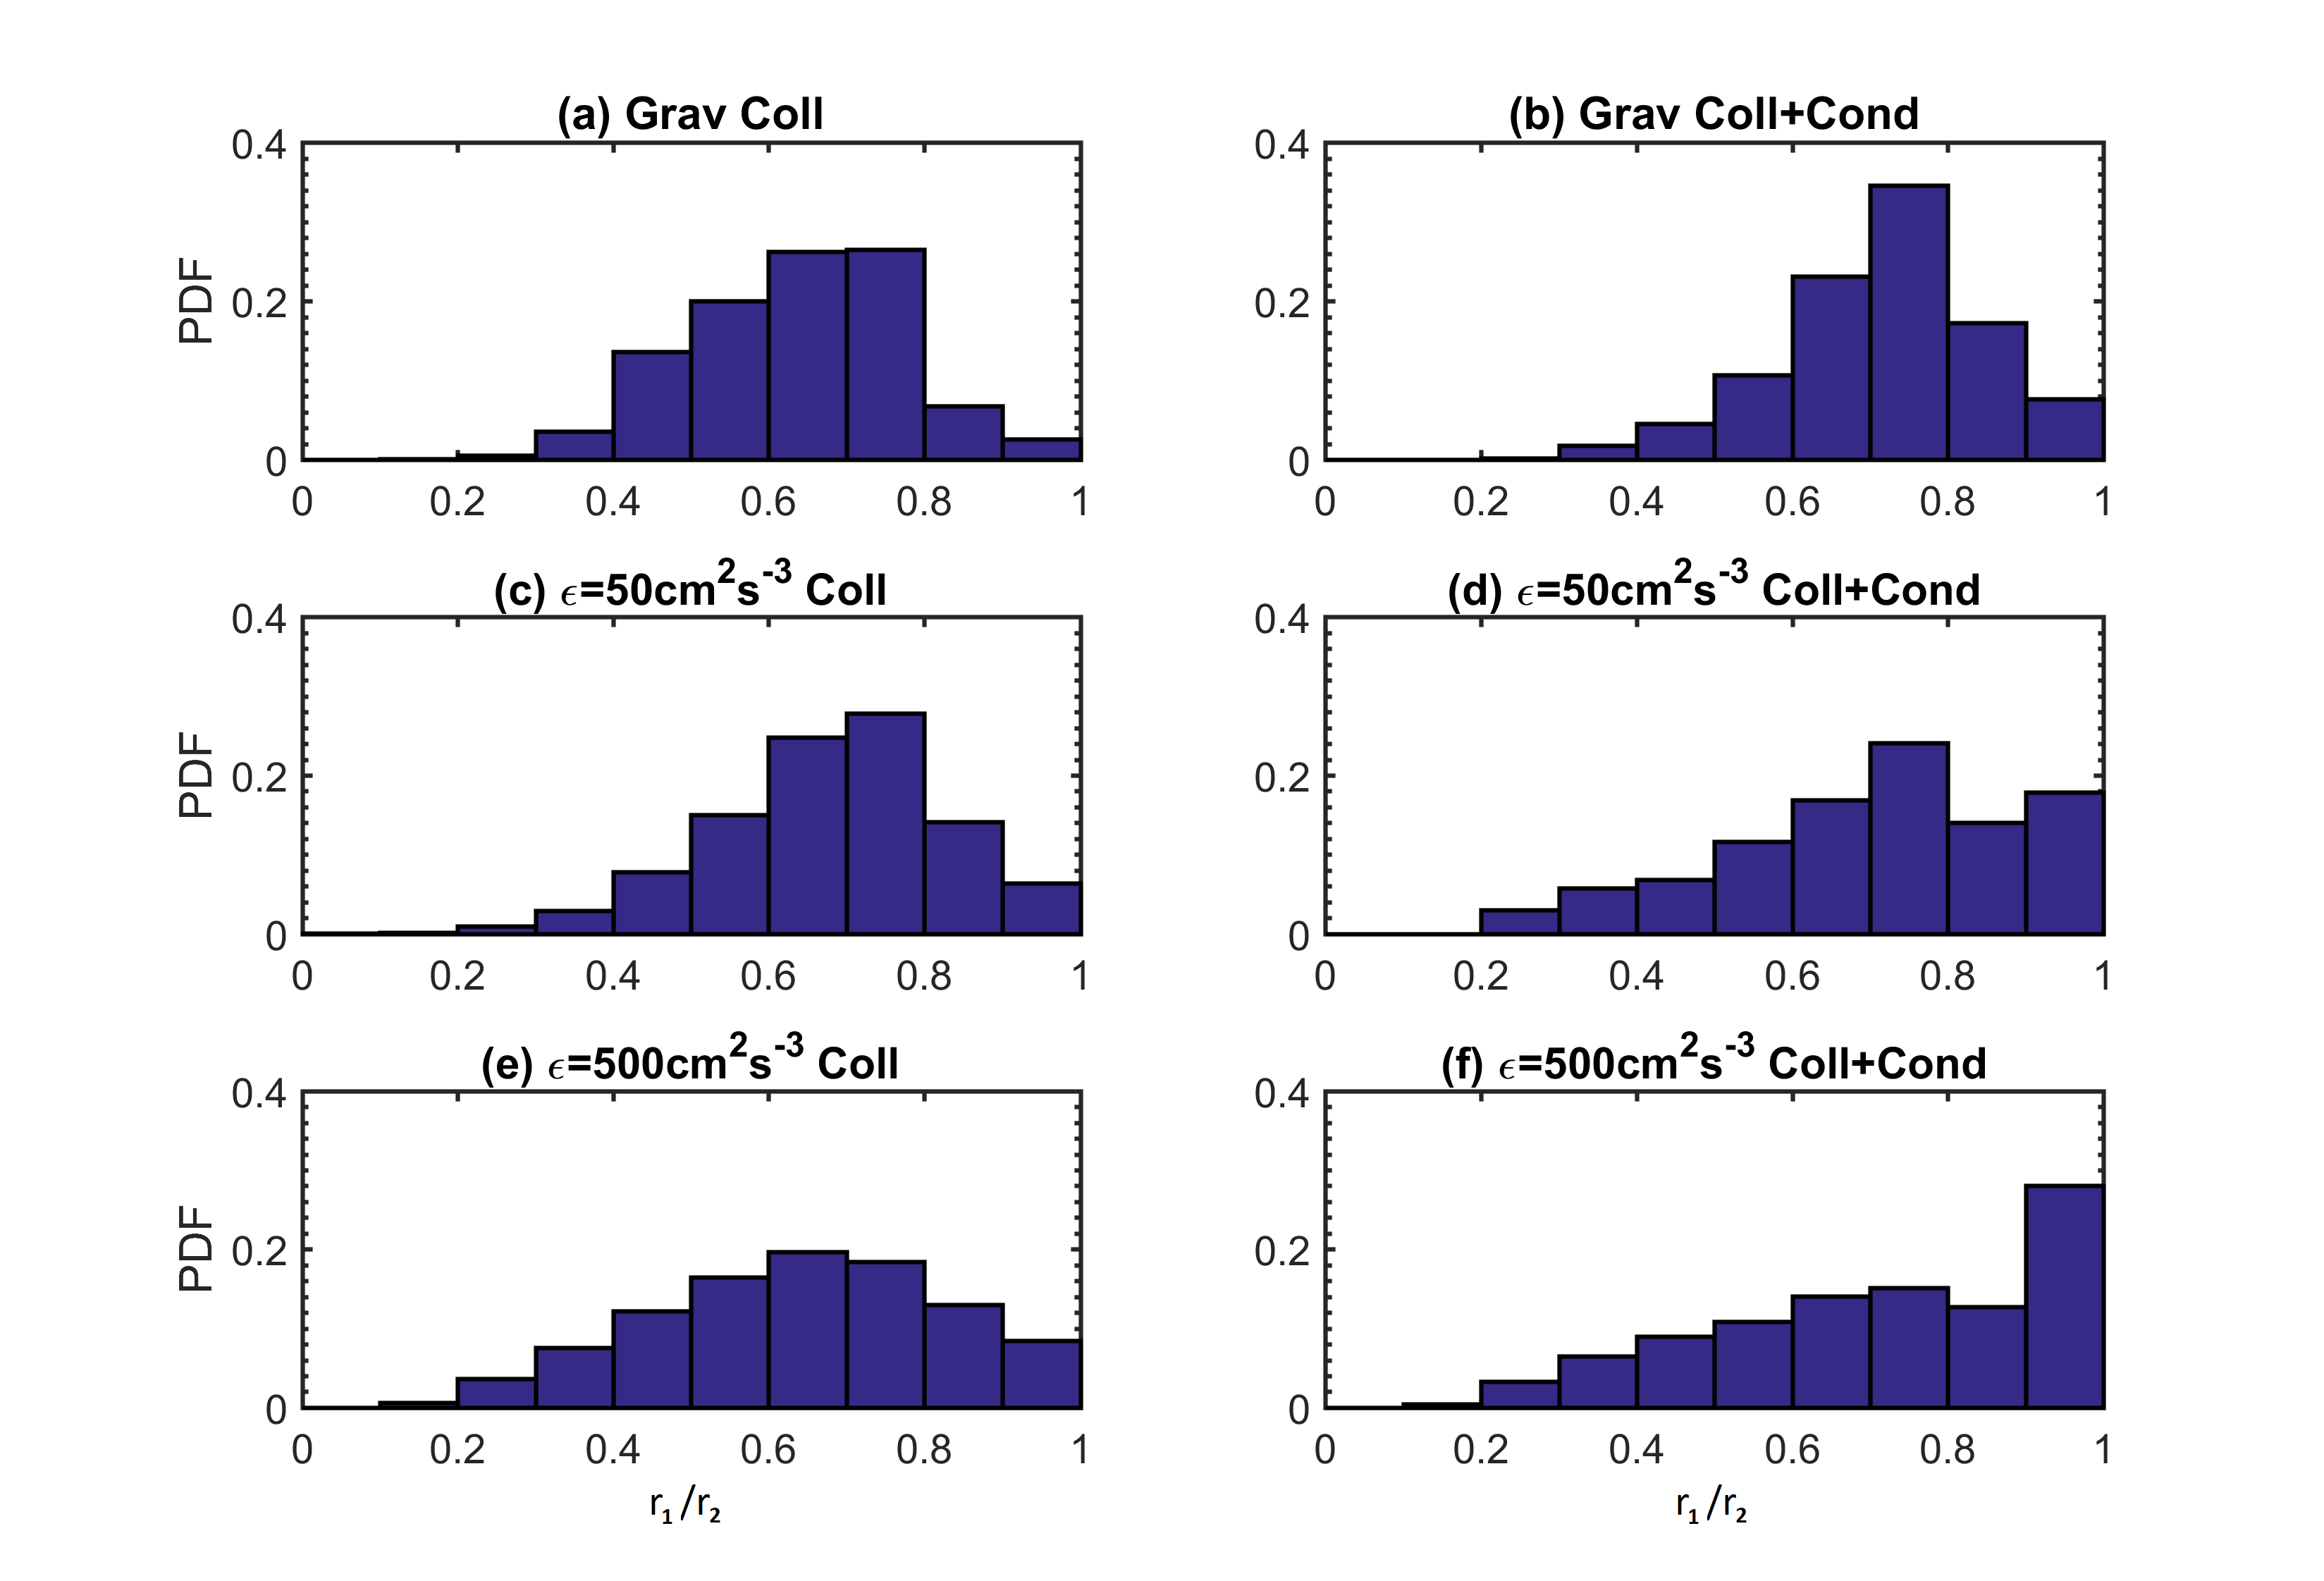
\includegraphics[width=0.8\textwidth]{Figures/Chap4/PDF_COLL.png}
\caption{Probability distribution function (PDF) of collisions with respect to $r_1/r_2$ at three different flow conditions (first row: pure gravity, second row: weak turbulence, third row: strong turbulence). Results from the collision-only experiments (the left column) and the condensation-collision experiments (the right column) are shown for comparison}\label{fig03}
\end{figure}

The first mechanism of enhanced collision rate due to larger mean droplet sizes can also happen in the purely-gravitational case but will be offset by the inefficient gravitational collection process due to DSD narrowing by condensation. In turbulent cases, the condensational DSD produce similar-sized droplets to allow the turbulence-enhanced similar-sized collision process to act, leading to a positive feedback mechanism. Evidence for this hypothesis can be found by comparing the probability distribution function (PDF) of collisions with respect to $r_1/r_2$ (the radius ratio between the small droplet and big droplet in a droplet pair) in the collision-only and the collision-condensation experiments. As seen in Fig. \ref{fig03}, the PDF of collisions in either the weak turbulence or the strong turbulence cases become more flattened when condensation is included. In particular, the chance of similar-sized collisions ($r_1/r_2>0.9$) is substantially greater. On the contrary, a narrower PDF is found in the purely-gravitational case (Figs. \ref{fig03}(a) and \ref{fig03}(b)). Figure \ref{fig04} demonstrates the distributions of collision frequency and the collision enhancement due to condensation. It is found that in the purely-gravitational case the number of similar-sized collisions doubles in the condensation-collision experiment, which results from the increased number of similar-sized droplets introduced by condensation. It is obvious that increasing the intensity of turbulence further enhances these collisions. The similar-sized collisions increase by a factor of 3.5 in weak turbulence and a factor of 4.5 in strong turbulence. 

\begin{figure}[ht]
\centering
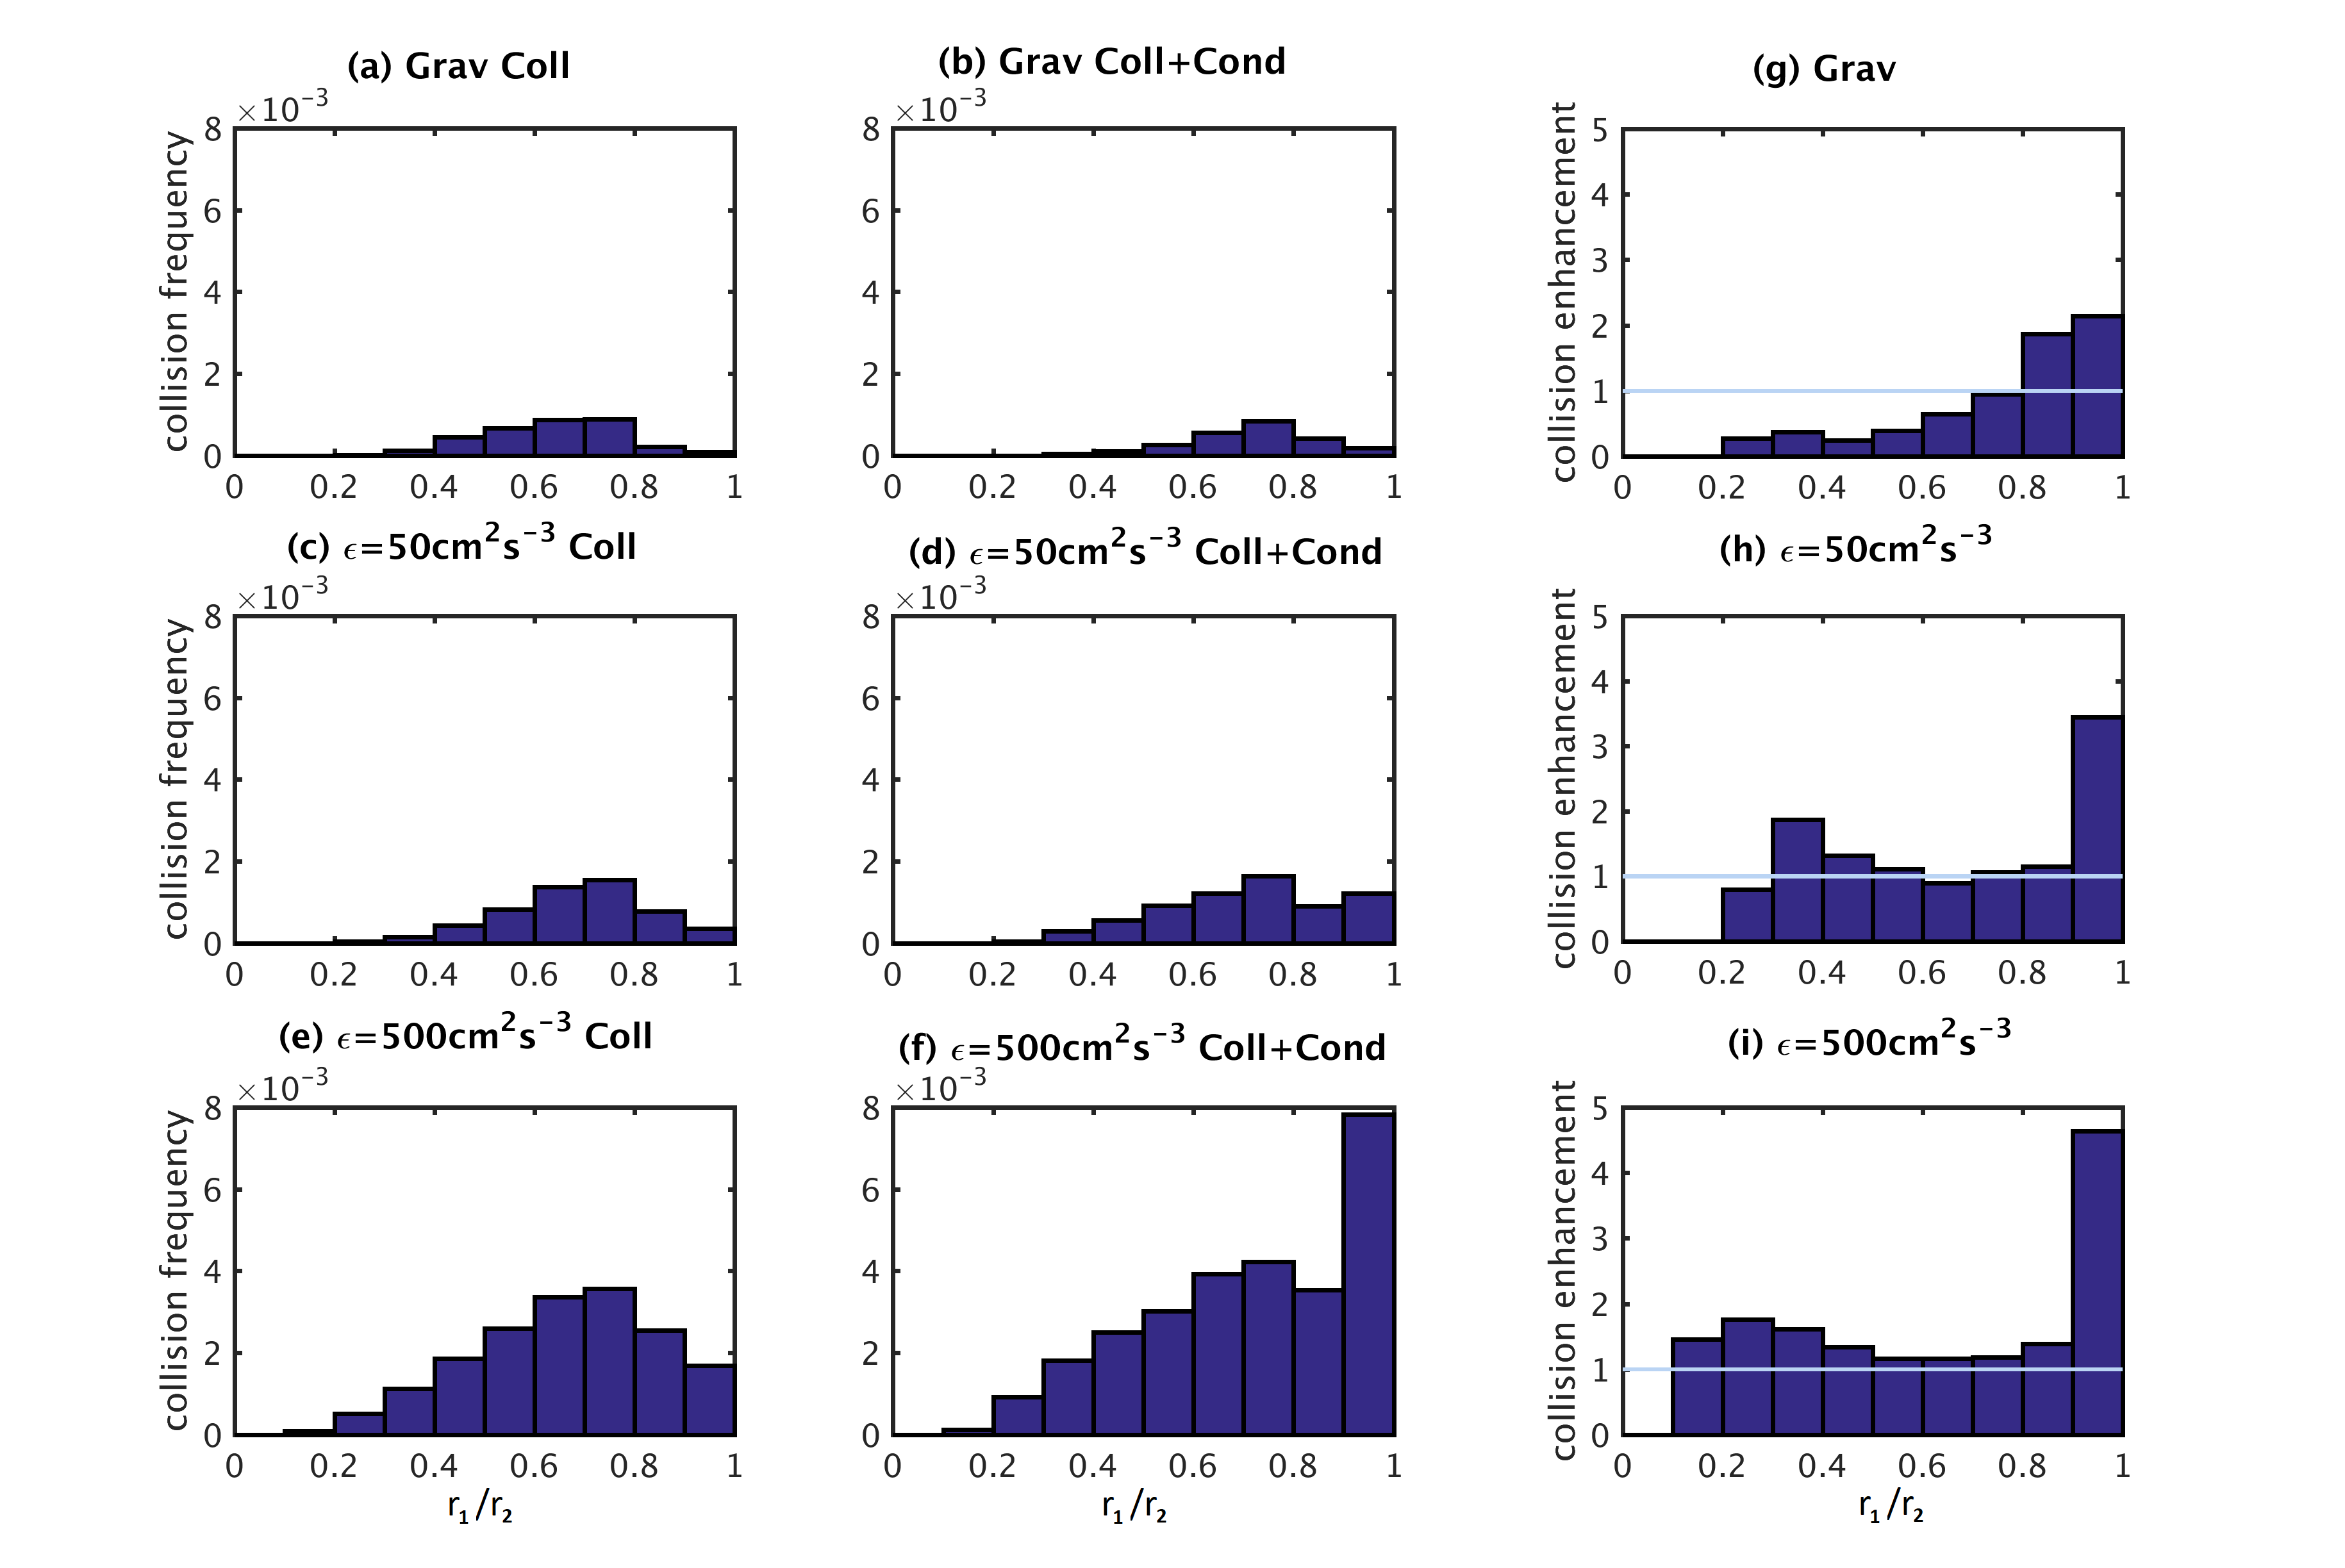
\includegraphics[width=0.8\textwidth]{Figures/Chap4/Freq_and_enhance.png}
\caption{Subplot (a)-(f) are the same as in Fig. \ref{fig03} but for the collision frequency ($cm^{-3} s^{-1}$) from different $r_1/r_2$ pairs.  Subplot (g)-(i) are the enhancement of collision frequency for different $r_1/r_2$ pairs due to the inclusion of condensation. The enhancement is calculated by taking the ratio of the collision frequency from the condensation-collision experiment and the collision-only experiment. Results from three different flow conditions are demonstrated.}\label{fig04}
\end{figure}

In the small r-ratio range ($r_1/r_2<0.7$), the total collisions in the purely-gravitational case are lowered by more than half due to a reduced number of those droplet pairs (Fig. \ref{fig04}(g)). However, in the turbulent cases, the collision frequency instead experiences a mild increase compared to the collision-only experiment. This increase is due to the fact that condensation increases the population of medium-sized droplets ($r=10-20 \mu m$) and turbulence continues to enhance the collisions of these droplets. The abundant number of those medium-sized droplets boosts the number of similar-sized collisions by turblence to produce larger droplets. Meanwhile, the larger size from growth by condensation substantially increases the chance of those droplets to be collected by other larger droplets. Furthermore, the formation of large droplets due to the turbulence-enhanced collisions in turn contributes to the growing collector droplet population, thus further increasing the chance of these medium-sized droplets to be collected. In the purely gravitational case, this process is inhibited by the insignificant similar-sized collisions in spite of their number being doubled from the collisional-only case.

To further illustrate the influence of turbulence on the enhancement of the condensation-induced collisions, we have studied the impact of condensation on the evolution of the number of droplet pairs. We divided the droplet pairs into two groups: the similar-sized pair group with $r/R>0.7$ and the different-sized pair group with $r/R \leq 0.7$. We then calculated the total number of droplet pairs within the two groups. By comparing the results from the collision-only experiments and the collision-condensaction experiments, we are able to separate the enhancement of collision rate solely due to turbulence and the enhancement directly associated with the inclusion of condensational growth. 

Figure \ref{fig05} shows the time evolution of the total number of droplet pairs for the two groups in the domain. For the convenience of comparison among the three turbulent cases, the pair numbers are calculated based on the droplet number concentration ($cm^{-3}$). For example, for the droplet pair of $r_1$ and $r_2$ with concentrations of $n_{d1}$ and $n_{d2}$, the pair number is $n_{d1}n_{d2}$ if $r_1 \neq r_2$ and $\frac{n_{d1}n_{d2}}{2}$ if $r_1 = r_2$. Therefore the unit of the pair number is in $cm^{-6}$. It is found that in the collision-only experiment the number of different-sized droplet pairs stays relatively constant (Fig. \ref{fig05}(a)). Meanwhile, the number of similar-sized droplets undergoes only a weak decay (Fig. \ref{fig05}(c)). Compared to the pure gravity case, turbulence effectively accelerates similar-sized collisions, while the enhancement of different-sized collisions is relatively small. On the one hand, the turbulence enhancement of similar-sized collisions is due to the fact that turbulence has a stronger effect on the similar-sized collision efficiency \citep{Chen2018}. On the other hand, it has been found that turbulence clustering effects are more significant for droplets of similar sizes \citep{Chen2016}. They tend to cluster in the same regions of the flow because of similar droplet inertia and terminal velocities. This effect has been confirmed previously in a number of studies \citep[e.g., ][]{Ayala2008a, Franklin2005} and is especially pronounced for large droplets. The reason is that small droplets have small Stokes numbers, and they adjust very quickly to changes in the flow and therefore behave more like fluid tracers than inertial droplets. Consequently, with growing droplet size, turbulence clustering of similar-sized droplets becomes more significant and the number of similar-sized pairs undergo an accelerated decline. This can be seen on Fig. \ref{fig05}(c) where the curve of the turbulent case deviates from the pure-gravitational case.

By contrast, in the condensation-collision experiment the trend of the number of droplet pairs behaves in a more complex fashion due to the inclusion of condensation. As illustrated by Fig. \ref{fig05}(b) and (d), the droplet growth experiences two different stages. The number of different-sized pairs significantly decreases in the first two minutes mainly due to the rapid condensational growth of droplets with $r < 15 \mu m$. This is demonstrated in Fig \ref{fig02} where the droplet number concentration for $r < 15 \mu m$ quickly reduces from larger than $1cm^{-3}$ to below $0.001cm^{-3}$ in the first two minutes, while the production of large droplets is still negligible. Concurrently, the number of similar-sized droplets significantly increases during the first two minutes and steadily decreases thereafter (Fig. \ref{fig05}(d)). The large increase of similar-sized pairs in the collision-condensation experiments during the first two minutes significantly increases the number of turbulent-enhanced similar-sized collisions. After two minutes, the condensational effect diminishes and the collision-coalescence process takes over in modulating the droplet pair population. The subsequent decline of the number of similar-sized pairs and the increase in the number of the different-sized pairs mainly arise from the collision-coalescence process.


\begin{figure}[h]
\centering
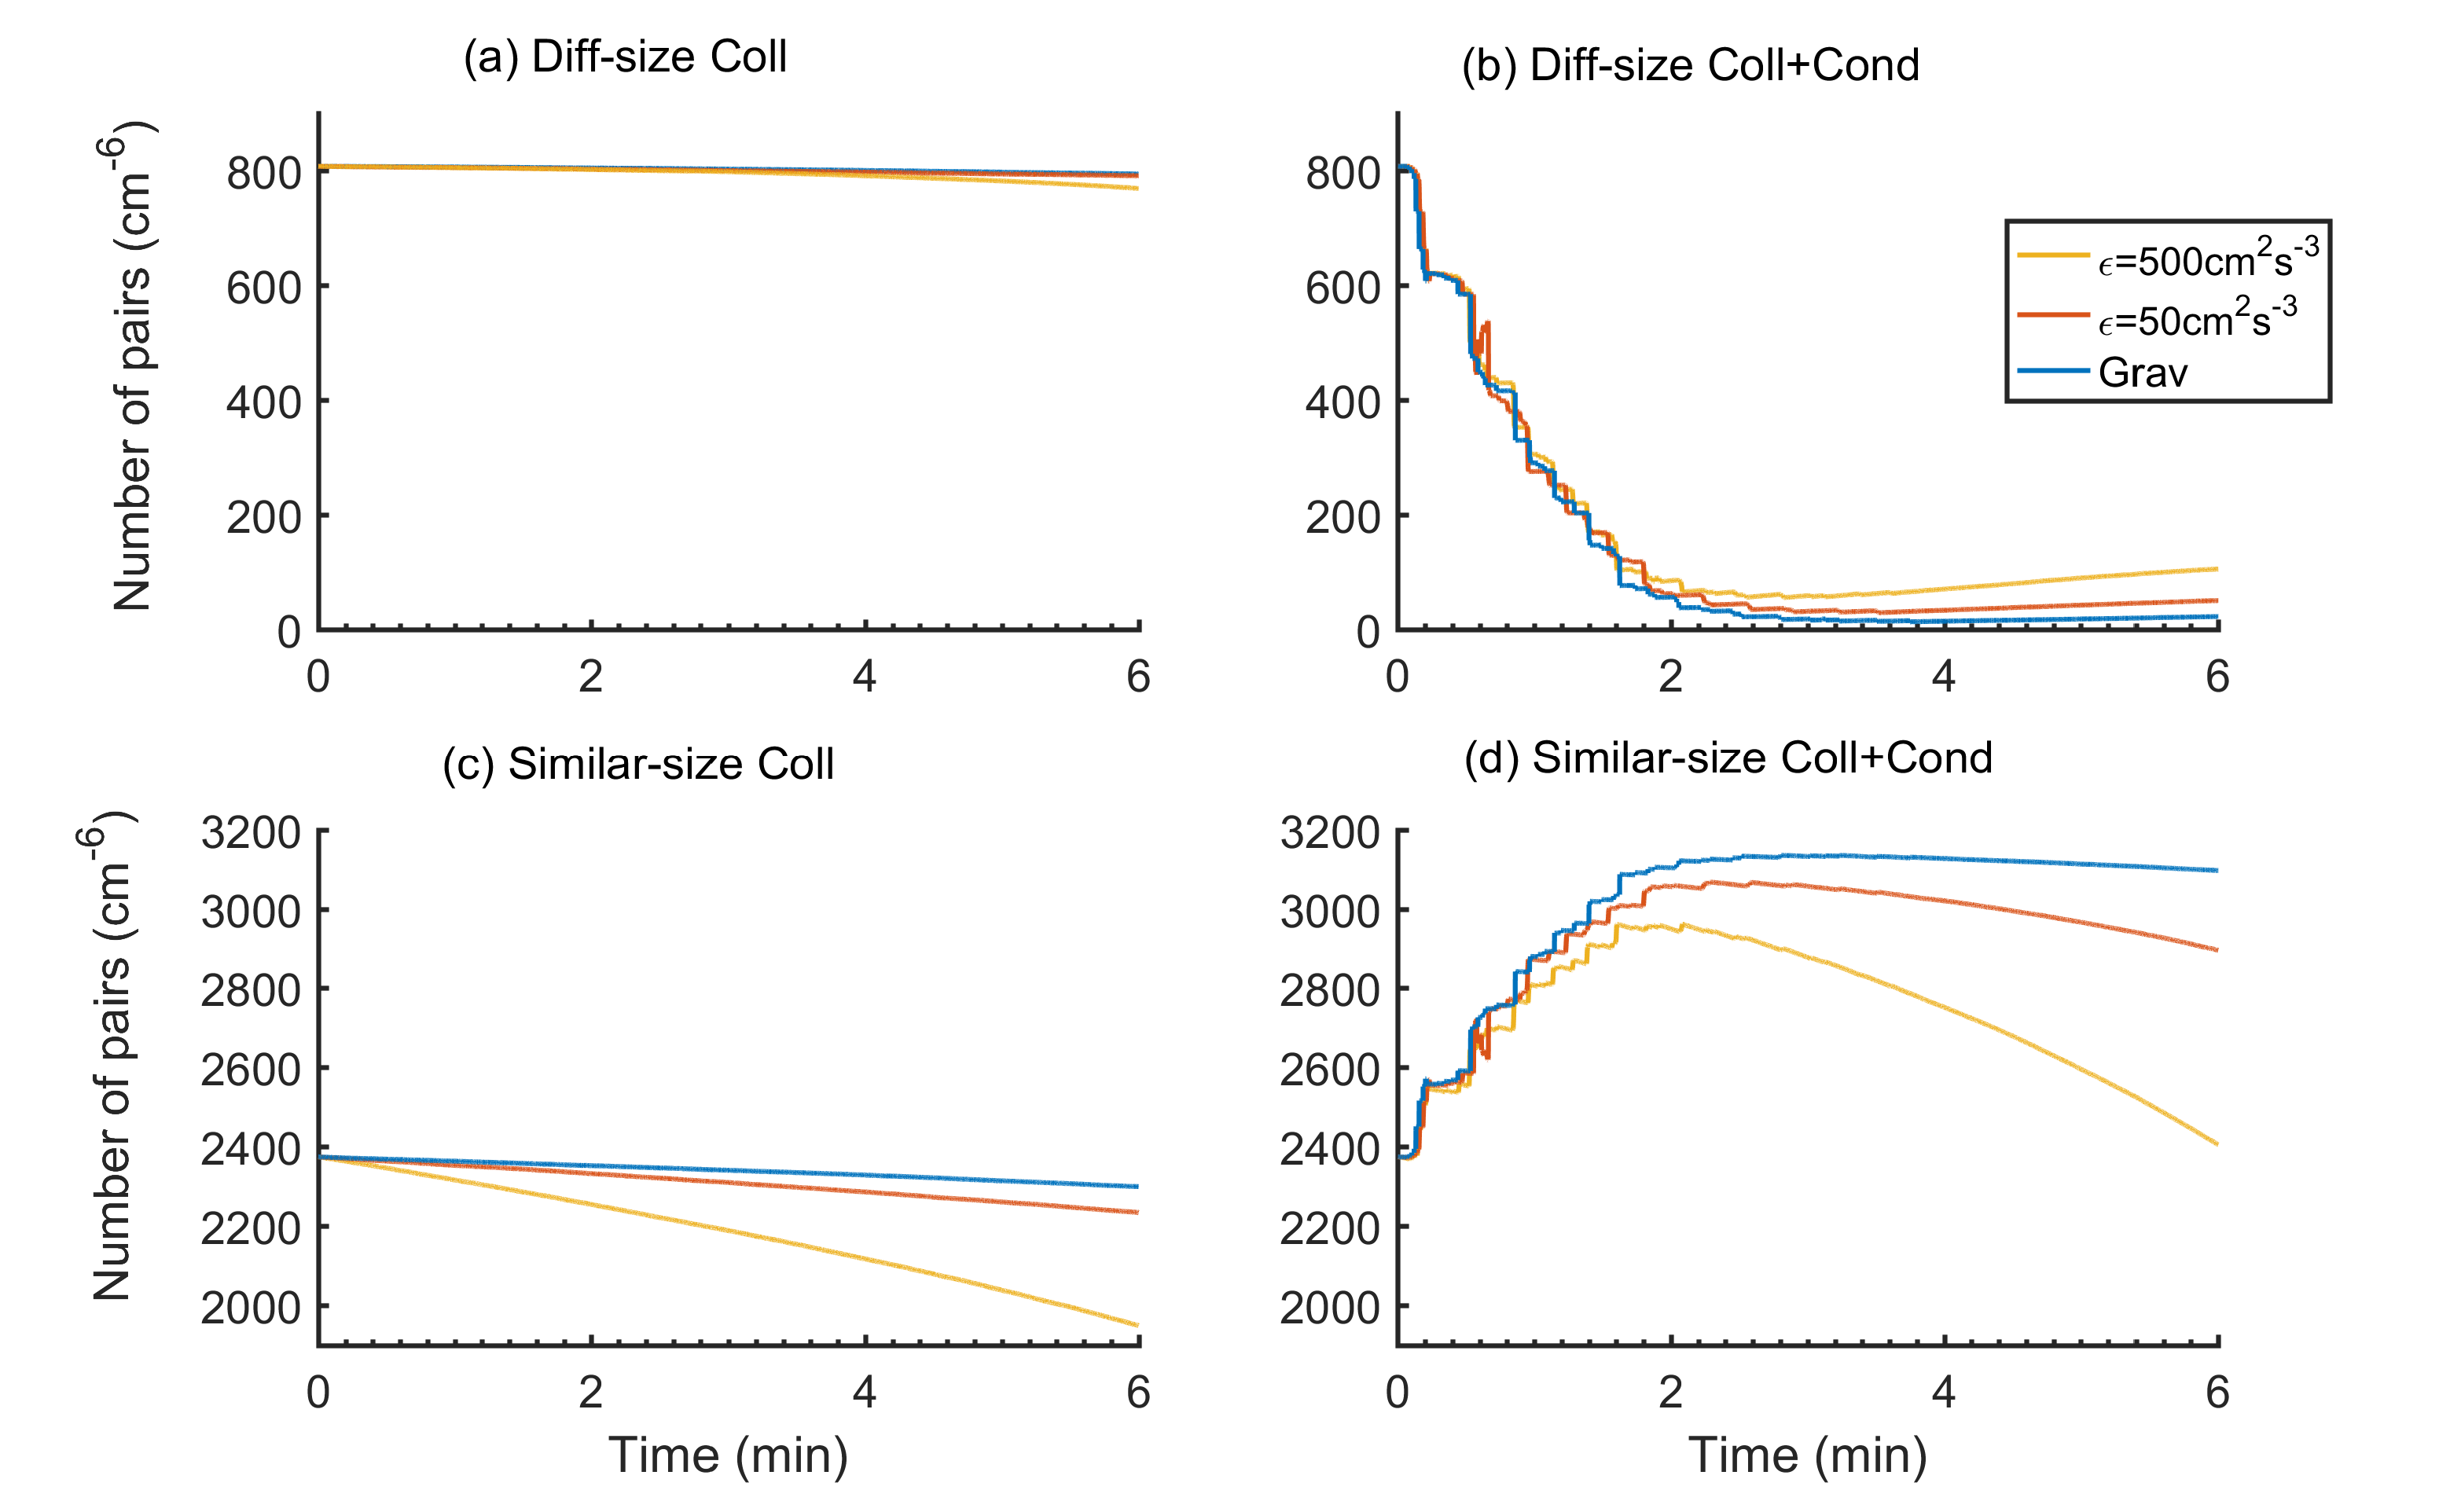
\includegraphics[width=0.8\textwidth]{Figures/Chap4/Pair_numbers.png}
\caption{Time evolution of the number of pair combinations for (a) the different-sized droplets ($r/R \leq 0.7$) and (c) the similar-sized droplets ($r/R>0.7$) in the collision-only experiments, and (b) the different-size droplets and (d) the similar-sized droplets in the condensation-collision experiments. The pair combination is computed using the droplet number concentration ($cm^{-3}$), therefore the unit is in $cm^{-6}$. The color denotes the three different flow conditions which are shown in the legend.}\label{fig05}
\end{figure}

\section{Conclusion} \label{sec:ch4_conclusion} %% \conclusions[modified heading if necessary]
This work provides the first DNS study to explicitly resolve continuous droplet growth by condensation and collision in a turbulent environment. The results are expected to contribute toward resolving the warm-rain initiation problem. 

Results from the condensation-only, collision-only, and condensation-collision experiments are compared to examine the contribution to the DSD broadening by the individual process and by the combined processes acting in concert. Three different flow environments (still air, weak turbulence, and strong turbulence) are investigated to scrutinize the impact of turbulence in the condensational-induced collisions. By comparing the collision frequencies of the collision-only experiment and the condensation-collision experiment, it is found that condensational growth boosts the collisions when the flow is turbulent and slows down the collisions for the case of still air. 

In the purely-gravitational experiment, the abundant similar-sized droplets generated by condensation inhibit the gravitational collection process, and the collision frequency of $r_1/r_2<0.7$ reduces by half. As a result, the number concentration of droplet larger than 35 $\mu m$ remains lower than 0.001 $cm^{-3}$ throughout the simulation. 

In the turbulence experiments, a greater number of large droplets are produced, and their appearance occurs faster as turbulence intensifies, implying an effective turbulence impact on droplet size broadening. Furthermore, droplets larger than 35 $\mu m$ form 1-2 minutes earlier in the collision-condensation experiments. It follows that these droplets appear as early as the 3rd minute in strong turbulence situation. This result suggests that a sophisticated model that takes into account both the turbulence-enhanced collisions and condensational-induced collisions under the effect of turbulence should be used to study the cloud droplet spectrum broadening and rain formation.

\acknowledgments
We would like to acknowledge Dr. Paul A. Vaillancourt from Environment and Climate Change Canada for providing the original DNS code and offering constant help in this project. We also thank Dr. Jorgen Jensen and Dr. Hugh Morrison from NCAR for their valuable discussions. Special thanks to Dr. Yeti Li for his insightful comments in shaping the first draft of this paper. We would also like to thank Dr. Brian Dobbins and Dr. Jeremy Sauer from NCAR for their generous help in improving the code performance. L. Xue appreciates the support of Beijing Weather Modification Office through Beijing Municipal Science and Technology Commission (Grant No.D171100000717001). We also acknowledge the support of the Natural Sciences and Engineering Research Council of Canada (NSERC). Computations were made on supercomputer Cheyenne (doi:10.5065/D6RX99HX) provided by NCAR's Computational and Information Systems Laboratory, sponsored by the National Science Foundation and on supercomputer Cedar provided by WestGrid (www.westgrid.ca) and Compute Canada Calcul Canada (www.computecanada.ca).

\cleardoublepage 


%========== Chapter 5 
\typeout{}
\resetdatestamp

\chapter{Conclusion and future directions}\label{sec:ch5}

\newpage

In this dissertation, we conducted direct numerical simulation (DNS) studies of the effect of turbulence on accelerating the growth of cloud droplets in the early stage of shallow cloud development, particularly inside the adiabatic cloud core. Numerous sets of numerical experiments were performed to study the impact of turbulence on droplet geometric collisions, droplet hydrodynamic interaction, and the interactions of collision and condensation. 

In past studies, the turbulence has been shown to exert a positive impact on droplet growth and accelerates the formation of warm rain. It has been widely accepted that turbulence enhances droplet collision statiscs through the effects of clustering of droplets, increasing droplet relative motion, and modifying the response of the droplet to the local disturbance flow. The three corresponding collision statistics are the droplet radial distribution function, the radial relative velocity, and the collision efficiency. The effects of turbulence on these three statistics are not the same. Specifically, our results show that the turbulence enhancement through the clustering effect and the relative motion effect is weaker than the enhancement of collision efficiency. Because of the importance of the collision efficiency effect, an accurate parameterization is required. Parameterizations such as \citet{Riemer2005}, \citet{Xue2008}, and \citet{Franklin2008} on the droplet collision kernel based on the lookup table of gravitational collision efficiencies are inaccurate. Additionally, the parameterizations based on DNS studies such as \citet{Franklin2007} and \citet{Ayala2008b} included the Reynolds number as an important parameter. However, in Chapter \ref{sec:ch2} it was demonstrated that the Reynolds number from DNS, which is calculated based on the computational domain size and thus is entirely artificial, has a secondary effect on the droplet collision statistics relative to the local dissipation rate and the inertial response of the droplet to the local flow (i.e., the Stokes number). The physical reason for our finding is that the scale of turbulence affecting droplet collisions is on the order of the mean separation distance between cloud droplets, which is of the order of the Kolmogorov length scale in cumulus clouds and far below our smallest computational domain size. It follows that the computational $R_\lambda$ becomes irrelevant and the turbulence can be characterized by the dissipation rate alone. A new parameterization for the turbulent geometric collision kernel that excludes the Reynolds number is therefore propsed. 

To model the effect of turbulence on the evolution of the droplet size distribution (DSD), droplet condensational growth must be included in addition to the collisional growth. One of the most intriguing results in Chapter \ref{sec:ch4} is that in the case of pure condensation, the effect of turbulence is small. However, the interplay between condensation and collision in broadening the DSD in turbulence is found to be substantial. The main reason is that condensation growth leads to a narrow DSD with more similar-sized droplets and the turbulence enhancement of collisions is particularly strong for similar-sized drop pairs.

Finally we remark on the limitation of this study and some suggestions for future work. It has been found that the evolution of the DSD and the rain formation time highly depend on the initial shape of the DSD and the droplet number concentration. Therefore, simulations of different initial DSDs are to be conducted to better understand its dependency. In addition, the initial DSD used in this study is taken from flight observations which represent an average over a long sampling time and a wide sampling volume. In this case, the initial DSD is not guaranteed to be representative of the steady-state DSD from aerosol activation and condensational growth in adiabatic cloud cores. However, with the continuous advancement of in-situ and laboratory measurement technology such as HOLO-DEC \citep{GRL2017} and PI chamber \citep{Desai2018}, representative sampling of the DSD near the cloud base inside adiabatic cores may be possible in the near future. It is also desirable to include the aerosol activation process to enable cloud particles to grow from the very beginning (i.e., dry aerosols in sub-cloud regions). Besides, the model can also be modified to study other microphysics processes such as ice nucleation which is poorly parameterized for deep convective clouds and cirrus clouds, and particle electrification which is potentially important in aerosol scavenging and droplet collisions.  

\cleardoublepage 


%========== Appendices
%\appendix

%%==========
%\typeout{}
%\input{sections/A-A}

%%==========
%\typeout{}
%\input{sections/A-B}


%========== Bibliography
\typeout{}
\begin{singlespace}
   \bibliographystyle{ametsoc2014}
  \bibliography{ThesisBib}
\end{singlespace}

\end{document}
